\documentclass[a4paper, 12pt]{article}

\usepackage[portuges]{babel}
\usepackage[utf8]{inputenc}
\usepackage{amsmath}
\usepackage{indentfirst}
\usepackage{graphicx}
\usepackage{multicol,lipsum}
\usepackage{booktabs}
\usepackage{longtable}
\usepackage{graphicx}
\usepackage{pst-pdf}
\usepackage{listings}
\usepackage{xcolor}

\lstset { %
	language=C++,
	backgroundcolor=\color{black!5}, % set backgroundcolor
	basicstyle=\footnotesize,% basic font setting
}

\begin{document}
	%\maketitle
	
	\begin{titlepage}
		\begin{center}
			
			%\begin{figure}[!ht]
			%\centering
			%\includegraphics[width=2cm]{c:/ufba.jpg}
			%\end{figure}
			
			\large{Társila Samille Santos da Silveira}\\ 
			\vspace{155pt}
			\vspace{95pt}
			\textbf{\LARGE{ Análise Empírica de Algoritmos de Ordenação  }}\\
			%\title{{\large{Título}}}
			\vspace{3,5cm}
		\end{center}
		
		
		
		
		\begin{center}
			\vspace{\fill}
			Brasil\\
			2020, v-1.0
		\end{center}
	\end{titlepage}
	%%%%%%%%%%%%%%%%%%%%%%%%%%%%%%%%%%%%%%%%%%%%%%%%%%%%%%%%%%%
	
	% % % % % % % % %FOLHA DE ROSTO % % % % % % % % % %
	
	\begin{titlepage}
		\begin{center}
			
			%\begin{figure}[!ht]
			%\centering
			%\includegraphics[width=2cm]{c:/ufba.jpg}
			%\end{figure}
			
			\large{Társila Samille Santos da Silveira}\\ 
			\vspace{15pt}
			
			\vspace{85pt}
			
			\textbf{\LARGE{Análise empírica de algoritmos}}
			\title{\large{Título}}
			%	\large{Modelo\\
			%   		Validação do modelo clássico}
			
		\end{center}
		\vspace{1,5cm}
		
		\begin{flushright}
			
			\begin{list}{}{
					\setlength{\leftmargin}{4.5cm}
					\setlength{\rightmargin}{0cm}
					\setlength{\labelwidth}{0pt}
					\setlength{\labelsep}{\leftmargin}}
				
				\item Relatório técnico apresentado à disciplina de Estrutura de Dados Básicas I, como requisito parcial para obtenção de nota referente à unidade I.
				
				
			\end{list}
		\end{flushright}
	\vspace{3cm}
\begin{center}{}
	
	
	
	\item Universidade Federal do Rio Grande do Norte - UFRN \
	\item Instituto Metrópole Digital - IMD \
	\item Bacharelado em Tecnologia da Informação\
	
\end{center}		


		\begin{center}
					\vspace{\fill}
		Brasil\\
		2020, v-1.0
		\end{center}
	\end{titlepage}
	\newpage
	% % % % % % % % % % % % % % % % % % % % % % % % % %
	\newpage
	\tableofcontents
	\thispagestyle{empty}
	
	\newpage
	\pagenumbering{arabic}
	% % % % % % % % % % % % % % % % % % % % % % % % % % %
	\section{Introdução}
	
		Este relatório objetiva realizar análises e comparações de algoritmos de ordenação eles foram executadas em um mesmo computador, no sistema operacional Ubutu. Todos os valores foram registrados em tabelas e plotados em gráficos, permitindo fácil comparação.\\
		\indent
		Nas seções seguintes, é apresentado o método seguido, abrangendo os materiais e ferramentas utilizadas; depois, são mostrados os resultados obtidos e, por fim, as discussões geradas a partir deles. O único apêndice traz a implementação em C++ dos algoritmos escolhidos.
	

	
	
	\section{Metodologia}
		
		\subsection{Materiais utilizados}
		
		\subsubsection{Computador}
	

		\begin{itemize}
		
		\item Computador: Acer Aspire-A315-42G
		
		\item Especificações: 
			\subitem Processador IAMD® Ryzen 5 3500u gfx × 8 
			\subitem 2 x 8GB DDR4 
			\subitem HD de 1T GB
			\subitem Radeon 540X Series (POLARIS12, DRM 3.35.0, 5.4.0-47-generic, LLVM 10.0.0) / AMD® Raven 
	\item 	Sistema Operacional e suas Especificações: 
\subitem GNU/Linux

\subsubitem Ubuntu 20.04.1 LTS(x86-64)
Kernel 3.36.3 

	\end{itemize}
	

	



		\subsubsection{Ferramentas de programação}
	Os quatro algoritmos escolhidos foram implementados na linguagem C++, padrão ISO/IEC 14882:2011, ou simplesmente C++11.\\
	\indent Os códigos foram compilados pelo CMake, uma família de ferramentas de plataforma cruzada de código aberto projetada para construir, testar e empacotar software. CMake é usado para controlar o processo de compilação do software usando uma plataforma simples e arquivos de configuração independentes do compilador, e gerar makefiles e espaços de trabalho nativos que podem ser usados no ambiente de copilação de sua escolha. Foi utilizado:
	
	\indent 	$>~$  cmake -S . -Bbuild  \\
		\indent $>$ cd build  \\
		\indent $>$ make\\
	
	\indent A biblioteca chrono3 foi responsável pelas medições do tempo de execução.
	
	\subsection{Método de comparações }
	Os algoritmos foram comparados segundo o critério de tempo de execução em relação ao tamanho do array.
	
\indent Para gerar o gráfico de 25 pontos, o vetor inicial começou com 10.000 e foi incrementado de 40mil em 40mil até chegar em 1.010.000 elementos.

\indent Foi implementado e analisado sete algoritmos. São eles: insertion
sort, selection sort, bubble sort, shell sort, quick sort, merge sort e radix sort (LSD).



\indent Com relação a organização das amostras foi simulado seis situações:



\begin{enumerate}

\item  arranjos com elementos em ordem não decrescente,
\item  arranjos com elemento em ordem não crescente,
\item  arranjos com elementos 100\% aleatórios,
\item  arranjos com 75\% de seus elementos em sua posição definitiva,
\item  arranjos com 25\% de seus elementos em sua posição definitiva, e
\item  arranjos com 50\% de seus elementos em sua posição definitiva.
\end{enumerate}



	\section{Resultados}
		\subsection{Tabelas - por algoritmo}


		
\subsubsection{Insertion}
A Tabela \ref{tab:insertion1-table} e \ref{tab:insertion2-table}  apresenta os resultados dos testes realizados com o algoritmo Insertion sort em diferentes situações de amostra, o resultado de tempo está em milissegundos.

% Please add the following required packages to your document preamble:
% \usepackage{booktabs}
% \usepackage{longtable}
% Note: It may be necessary to compile the document several times to get a multi-page table to line up properly
\begin{longtable}[c]{@{}rrrr@{}}
				\caption{Insertion Sort (tempo em ms)}
	\label{tab:insertion1-table}\\
	\toprule
	\multicolumn{1}{l}{\textbf{Tamanho do Array}} & \multicolumn{1}{c}{\textbf{Crescente}} & \multicolumn{1}{c}{\textbf{Decrescente}} & \multicolumn{1}{c}{\textbf{Aleatório}} \\* \midrule
	\endfirsthead
	%
	\endhead
	%
	\multicolumn{1}{|r|}{10000}                   & \multicolumn{1}{r|}{550,377}           & \multicolumn{1}{r|}{101,956}             & \multicolumn{1}{r|}{75,482}            \\* \midrule
	\multicolumn{1}{|r|}{50000}                   & \multicolumn{1}{r|}{1077,17}           & \multicolumn{1}{r|}{2.421,970}           & \multicolumn{1}{r|}{1.583,800}         \\* \midrule
	\multicolumn{1}{|r|}{90000}                   & \multicolumn{1}{r|}{3469,59}           & \multicolumn{1}{r|}{7.833,780}           & \multicolumn{1}{r|}{5.404,500}         \\* \midrule
	\multicolumn{1}{|r|}{130000}                  & \multicolumn{1}{r|}{7462,2}            & \multicolumn{1}{r|}{16.256,000}          & \multicolumn{1}{r|}{11.225,900}        \\* \midrule
	\multicolumn{1}{|r|}{170000}                  & \multicolumn{1}{r|}{12557,3}           & \multicolumn{1}{r|}{27.856,500}          & \multicolumn{1}{r|}{18.535,200}        \\* \midrule
	\multicolumn{1}{|r|}{210000}                  & \multicolumn{1}{r|}{18880,7}           & \multicolumn{1}{r|}{42.301,900}          & \multicolumn{1}{r|}{28.711,700}        \\* \midrule
	\multicolumn{1}{|r|}{250000}                  & \multicolumn{1}{r|}{27008,6}           & \multicolumn{1}{r|}{59.965,400}          & \multicolumn{1}{r|}{41.137,200}        \\* \midrule
	\multicolumn{1}{|r|}{290000}                  & \multicolumn{1}{r|}{36740,1}           & \multicolumn{1}{r|}{80.531,800}          & \multicolumn{1}{r|}{56.253,300}        \\* \midrule
	\multicolumn{1}{|r|}{330000}                  & \multicolumn{1}{r|}{47595,7}           & \multicolumn{1}{r|}{104.420,000}         & \multicolumn{1}{r|}{71.916,000}        \\* \midrule
	\multicolumn{1}{|r|}{370000}                  & \multicolumn{1}{r|}{59177,2}           & \multicolumn{1}{r|}{131.021,000}         & \multicolumn{1}{r|}{98.030,400}        \\* \midrule
	\multicolumn{1}{|r|}{410000}                  & \multicolumn{1}{r|}{72527,3}           & \multicolumn{1}{r|}{160.739,000}         & \multicolumn{1}{r|}{119.197,000}       \\* \midrule
	\multicolumn{1}{|r|}{450000}                  & \multicolumn{1}{r|}{88845,4}           & \multicolumn{1}{r|}{193.791,000}         & \multicolumn{1}{r|}{145.967,000}       \\* \midrule
	\multicolumn{1}{|r|}{490000}                  & \multicolumn{1}{r|}{104.553,000}       & \multicolumn{1}{r|}{229.605,000}         & \multicolumn{1}{r|}{173.334,000}       \\* \midrule
	\multicolumn{1}{|r|}{530000}                  & \multicolumn{1}{r|}{122.178,000}       & \multicolumn{1}{r|}{268.542,000}         & \multicolumn{1}{r|}{203.260,000}       \\* \midrule
	\multicolumn{1}{|r|}{570000}                  & \multicolumn{1}{r|}{142.547,000}       & \multicolumn{1}{r|}{315.684,000}         & \multicolumn{1}{r|}{226.165,000}       \\* \midrule
	\multicolumn{1}{|r|}{610000}                  & \multicolumn{1}{r|}{163.120,000}       & \multicolumn{1}{r|}{394.911,000}         & \multicolumn{1}{r|}{249.170,000}       \\* \midrule
	\multicolumn{1}{|r|}{650000}                  & \multicolumn{1}{r|}{183.942,000}       & \multicolumn{1}{r|}{465.972,000}         & \multicolumn{1}{r|}{275.138,000}       \\* \midrule
	\multicolumn{1}{|r|}{690000}                  & \multicolumn{1}{r|}{208.621,000}       & \multicolumn{1}{r|}{522.556,000}         & \multicolumn{1}{r|}{316.797,000}       \\* \midrule
	\multicolumn{1}{|r|}{730000}                  & \multicolumn{1}{r|}{232.146,000}       & \multicolumn{1}{r|}{590.953,000}         & \multicolumn{1}{r|}{377.368,000}       \\* \midrule
	\multicolumn{1}{|r|}{770000}                  & \multicolumn{1}{r|}{260.515,000}       & \multicolumn{1}{r|}{628.866,000}         & \multicolumn{1}{r|}{421.278,000}       \\* \midrule
	\multicolumn{1}{|r|}{810000}                  & \multicolumn{1}{r|}{288.769,000}       & \multicolumn{1}{r|}{693.121,000}         & \multicolumn{1}{r|}{447.360,000}       \\* \midrule
	\multicolumn{1}{|r|}{850000}                  & \multicolumn{1}{r|}{305.281,000}       & \multicolumn{1}{r|}{771.121,000}         & \multicolumn{1}{r|}{524.716,000}       \\* \midrule
	\multicolumn{1}{|r|}{890000}                  & \multicolumn{1}{r|}{335.134,000}       & \multicolumn{1}{r|}{818.266,000}         & \multicolumn{1}{r|}{649.251,000}       \\* \midrule
	\multicolumn{1}{|r|}{930000}                  & \multicolumn{1}{r|}{366.052,000}       & \multicolumn{1}{r|}{904.231,000}         & \multicolumn{1}{r|}{723.784,000}       \\* \midrule
	\multicolumn{1}{|r|}{970000}                  & \multicolumn{1}{r|}{399.564,000}       & \multicolumn{1}{r|}{928.554,000}         & \multicolumn{1}{r|}{741.000,000}       \\* \bottomrule
\end{longtable}
\begin{longtable}[c]{@{}rrrr@{}}
				\caption{Insertion Sort (tempo em ms)}
	\label{tab:insertion2-table}\\
	\toprule
	\multicolumn{1}{l}{\textbf{Tamanho do Array}} & \multicolumn{1}{c}{\textbf{75\% Aleatório}} & \multicolumn{1}{c}{\textbf{\begin{tabular}[c]{@{}c@{}}50\% \\ Aleatório\end{tabular}}} & \multicolumn{1}{c}{\textbf{\begin{tabular}[c]{@{}c@{}}25\% \\ Aleatório\end{tabular}}} \\* \midrule
	\endfirsthead
	%
	\endhead
	%
	\multicolumn{1}{|r|}{10000}                   & \multicolumn{1}{r|}{71,9663}                & \multicolumn{1}{r|}{83,2349}                                                           & \multicolumn{1}{r|}{44,6875}                                                           \\* \midrule
	\multicolumn{1}{|r|}{50000}                   & \multicolumn{1}{r|}{1575,7400}              & \multicolumn{1}{r|}{2097,1300}                                                         & \multicolumn{1}{r|}{1087,77}                                                           \\* \midrule
	\multicolumn{1}{|r|}{90000}                   & \multicolumn{1}{r|}{4963,9100}              & \multicolumn{1}{r|}{6730,4000}                                                         & \multicolumn{1}{r|}{3515,69}                                                           \\* \midrule
	\multicolumn{1}{|r|}{130000}                  & \multicolumn{1}{r|}{10505,3000}             & \multicolumn{1}{r|}{14155,9000}                                                        & \multicolumn{1}{r|}{7416,56}                                                           \\* \midrule
	\multicolumn{1}{|r|}{170000}                  & \multicolumn{1}{r|}{18269,3000}             & \multicolumn{1}{r|}{20408,5000}                                                        & \multicolumn{1}{r|}{12614,7}                                                           \\* \midrule
	\multicolumn{1}{|r|}{210000}                  & \multicolumn{1}{r|}{27249,7000}             & \multicolumn{1}{r|}{23833,7000}                                                        & \multicolumn{1}{r|}{19225,9}                                                           \\* \midrule
	\multicolumn{1}{|r|}{250000}                  & \multicolumn{1}{r|}{38286,6000}             & \multicolumn{1}{r|}{41619,8000}                                                        & \multicolumn{1}{r|}{27512,7}                                                           \\* \midrule
	\multicolumn{1}{|r|}{290000}                  & \multicolumn{1}{r|}{51730,9000}             & \multicolumn{1}{r|}{51795,8000}                                                        & \multicolumn{1}{r|}{37160,9}                                                           \\* \midrule
	\multicolumn{1}{|r|}{330000}                  & \multicolumn{1}{r|}{66350,6000}             & \multicolumn{1}{r|}{63412,8000}                                                        & \multicolumn{1}{r|}{48283,8}                                                           \\* \midrule
	\multicolumn{1}{|r|}{370000}                  & \multicolumn{1}{r|}{86469,8000}             & \multicolumn{1}{r|}{90323,5000}                                                        & \multicolumn{1}{r|}{60906,1}                                                           \\* \midrule
	\multicolumn{1}{|r|}{410000}                  & \multicolumn{1}{r|}{107734,0000}            & \multicolumn{1}{r|}{108305,0000}                                                       & \multicolumn{1}{r|}{74446,6}                                                           \\* \midrule
	\multicolumn{1}{|r|}{450000}                  & \multicolumn{1}{r|}{133323,0000}            & \multicolumn{1}{r|}{147413,0000}                                                       & \multicolumn{1}{r|}{89390,6}                                                           \\* \midrule
	\multicolumn{1}{|r|}{490000}                  & \multicolumn{1}{r|}{159320,0000}            & \multicolumn{1}{r|}{178700,0000}                                                       & \multicolumn{1}{r|}{105529}                                                            \\* \midrule
	\multicolumn{1}{|r|}{530000}                  & \multicolumn{1}{r|}{186991,0000}            & \multicolumn{1}{r|}{220332,0000}                                                       & \multicolumn{1}{r|}{124057}                                                            \\* \midrule
	\multicolumn{1}{|r|}{570000}                  & \multicolumn{1}{r|}{219251,0000}            & \multicolumn{1}{r|}{255489,0000}                                                       & \multicolumn{1}{r|}{143506}                                                            \\* \midrule
	\multicolumn{1}{|r|}{610000}                  & \multicolumn{1}{r|}{257619,0000}            & \multicolumn{1}{r|}{278879,0000}                                                       & \multicolumn{1}{r|}{164648}                                                            \\* \midrule
	\multicolumn{1}{|r|}{650000}                  & \multicolumn{1}{r|}{292809,0000}            & \multicolumn{1}{r|}{337602,0000}                                                       & \multicolumn{1}{r|}{209307}                                                            \\* \midrule
	\multicolumn{1}{|r|}{690000}                  & \multicolumn{1}{r|}{345894,0000}            & \multicolumn{1}{r|}{408861,0000}                                                       & \multicolumn{1}{r|}{233766}                                                            \\* \midrule
	\multicolumn{1}{|r|}{730000}                  & \multicolumn{1}{r|}{434744,0000}            & \multicolumn{1}{r|}{481184,0000}                                                       & \multicolumn{1}{r|}{261210}                                                            \\* \midrule
	\multicolumn{1}{|r|}{770000}                  & \multicolumn{1}{r|}{571000,0000}            & \multicolumn{1}{r|}{490971,0000}                                                       & \multicolumn{1}{r|}{280444}                                                            \\* \midrule
	\multicolumn{1}{|r|}{810000}                  & \multicolumn{1}{r|}{657000,0000}            & \multicolumn{1}{r|}{438604,0000}                                                       & \multicolumn{1}{r|}{310181}                                                            \\* \midrule
	\multicolumn{1}{|r|}{850000}                  & \multicolumn{1}{r|}{698000,0000}            & \multicolumn{1}{r|}{502607,0000}                                                       & \multicolumn{1}{r|}{339117}                                                            \\* \midrule
	\multicolumn{1}{|r|}{890000}                  & \multicolumn{1}{r|}{822000,0000}            & \multicolumn{1}{r|}{452795,0000}                                                       & \multicolumn{1}{r|}{379192}                                                            \\* \midrule
	\multicolumn{1}{|r|}{930000}                  & \multicolumn{1}{r|}{890000,0000}            & \multicolumn{1}{r|}{476458,0000}                                                       & \multicolumn{1}{r|}{417594}                                                            \\* \midrule
	\multicolumn{1}{|r|}{970000}                  & \multicolumn{1}{r|}{926000,0000}            & \multicolumn{1}{r|}{552236,0000}                                                       & \multicolumn{1}{r|}{4,52E+05}                                                          \\* \bottomrule
\end{longtable}

\subsubsection{Selection}
A Tabela \ref{tab:selection1-table} e \ref{tab:selection2-table}  apresenta os resultados dos testes realizados com o algoritmo Selection sort em diferentes situações de amostra, o resultado de tempo está em milissegundos.
% Please add the following required packages to your document preamble:
% \usepackage{booktabs}
% \usepackage{longtable}
% Note: It may be necessary to compile the document several times to get a multi-page table to line up properly
\begin{longtable}[c]{@{}rrrr@{}}
				\caption{Selection Sort (tempo em ms)}
	\label{tab:selection1-table}\\
	\toprule
	\multicolumn{1}{l}{\textbf{Tamanho do Array}} & \multicolumn{1}{c}{\textbf{Crescente}} & \multicolumn{1}{c}{\textbf{Decrescente}} & \multicolumn{1}{c}{\textbf{Aleatório}} \\* \midrule
	\endfirsthead
	%
	\endhead
	%
	\multicolumn{1}{|r|}{10000}                   & \multicolumn{1}{r|}{37,609}            & \multicolumn{1}{r|}{251,551}             & \multicolumn{1}{r|}{43,698}            \\* \midrule
	\multicolumn{1}{|r|}{50000}                   & \multicolumn{1}{r|}{667,644}           & \multicolumn{1}{r|}{6.326,880}           & \multicolumn{1}{r|}{844,853}           \\* \midrule
	\multicolumn{1}{|r|}{90000}                   & \multicolumn{1}{r|}{2.152,050}         & \multicolumn{1}{r|}{19.557,300}          & \multicolumn{1}{r|}{2.804,390}         \\* \midrule
	\multicolumn{1}{|r|}{130000}                  & \multicolumn{1}{r|}{4.342,840}         & \multicolumn{1}{r|}{40.984,400}          & \multicolumn{1}{r|}{5.675,910}         \\* \midrule
	\multicolumn{1}{|r|}{170000}                  & \multicolumn{1}{r|}{7.769,350}         & \multicolumn{1}{r|}{75.251,500}          & \multicolumn{1}{r|}{9.105,960}         \\* \midrule
	\multicolumn{1}{|r|}{210000}                  & \multicolumn{1}{r|}{11.987,100}        & \multicolumn{1}{r|}{118.257,000}         & \multicolumn{1}{r|}{13.858,000}        \\* \midrule
	\multicolumn{1}{|r|}{250000}                  & \multicolumn{1}{r|}{16.443,600}        & \multicolumn{1}{r|}{175.041,000}         & \multicolumn{1}{r|}{17.900,500}        \\* \midrule
	\multicolumn{1}{|r|}{290000}                  & \multicolumn{1}{r|}{23.194,300}        & \multicolumn{1}{r|}{238.020,000}         & \multicolumn{1}{r|}{23.277,200}        \\* \midrule
	\multicolumn{1}{|r|}{330000}                  & \multicolumn{1}{r|}{30.984,100}        & \multicolumn{1}{r|}{323.680,000}         & \multicolumn{1}{r|}{30.136,300}        \\* \midrule
	\multicolumn{1}{|r|}{370000}                  & \multicolumn{1}{r|}{39.758,700}        & \multicolumn{1}{r|}{390.678,000}         & \multicolumn{1}{r|}{39.653,400}        \\* \midrule
	\multicolumn{1}{|r|}{410000}                  & \multicolumn{1}{r|}{46.609,100}        & \multicolumn{1}{r|}{485.030,000}         & \multicolumn{1}{r|}{49.330,800}        \\* \midrule
	\multicolumn{1}{|r|}{450000}                  & \multicolumn{1}{r|}{57.374,500}        & \multicolumn{1}{r|}{513.363,000}         & \multicolumn{1}{r|}{62.570,100}        \\* \midrule
	\multicolumn{1}{|r|}{490000}                  & \multicolumn{1}{r|}{65.690,400}        & \multicolumn{1}{r|}{629.288,000}         & \multicolumn{1}{r|}{71.472,800}        \\* \midrule
	\multicolumn{1}{|r|}{530000}                  & \multicolumn{1}{r|}{75.679,300}        & \multicolumn{1}{r|}{673.056,000}         & \multicolumn{1}{r|}{83.609,700}        \\* \midrule
	\multicolumn{1}{|r|}{570000}                  & \multicolumn{1}{r|}{90.300,400}        & \multicolumn{1}{r|}{659.361,000}         & \multicolumn{1}{r|}{97.260,400}        \\* \midrule
	\multicolumn{1}{|r|}{610000}                  & \multicolumn{1}{r|}{101.356,000}       & \multicolumn{1}{r|}{105.012,000}         & \multicolumn{1}{r|}{110.160,000}       \\* \midrule
	\multicolumn{1}{|r|}{650000}                  & \multicolumn{1}{r|}{123.253,000}       & \multicolumn{1}{r|}{114.622,000}         & \multicolumn{1}{r|}{128.671,000}       \\* \midrule
	\multicolumn{1}{|r|}{690000}                  & \multicolumn{1}{r|}{150.585,000}       & \multicolumn{1}{r|}{133.372,000}         & \multicolumn{1}{r|}{165.380,000}       \\* \midrule
	\multicolumn{1}{|r|}{730000}                  & \multicolumn{1}{r|}{160.535,000}       & \multicolumn{1}{r|}{135.360,000}         & \multicolumn{1}{r|}{184.990,000}       \\* \midrule
	\multicolumn{1}{|r|}{770000}                  & \multicolumn{1}{r|}{195.979,000}       & \multicolumn{1}{r|}{150.631,000}         & \multicolumn{1}{r|}{212.639,000}       \\* \midrule
	\multicolumn{1}{|r|}{810000}                  & \multicolumn{1}{r|}{208.087,000}       & \multicolumn{1}{r|}{175.798,000}         & \multicolumn{1}{r|}{232.121,000}       \\* \midrule
	\multicolumn{1}{|r|}{850000}                  & \multicolumn{1}{r|}{223.211,000}       & \multicolumn{1}{r|}{213.962,000}         & \multicolumn{1}{r|}{242.870,000}       \\* \midrule
	\multicolumn{1}{|r|}{890000}                  & \multicolumn{1}{r|}{247.716,000}       & \multicolumn{1}{r|}{231.065,000}         & \multicolumn{1}{r|}{271.252,000}       \\* \midrule
	\multicolumn{1}{|r|}{930000}                  & \multicolumn{1}{r|}{266.839,000}       & \multicolumn{1}{r|}{261.714,000}         & \multicolumn{1}{r|}{294.587,000}       \\* \midrule
	\multicolumn{1}{|r|}{970000}                  & \multicolumn{1}{r|}{278.371,000}       & \multicolumn{1}{r|}{396.680,000}         & \multicolumn{1}{r|}{315.804,000}       \\* \bottomrule
\end{longtable}
% Please add the following required packages to your document preamble:
% \usepackage{booktabs}
% \usepackage{longtable}
% Note: It may be necessary to compile the document several times to get a multi-page table to line up properly
\begin{longtable}[c]{@{}rrrr@{}}
	\caption{Selection Sort (tempo em ms)}
	\label{tab:selection2-table}\\
	\toprule
	\multicolumn{1}{l}{\textbf{Tamanho do Array}} & \multicolumn{1}{c}{\textbf{75\% Aleatório}} & \multicolumn{1}{c}{\textbf{\begin{tabular}[c]{@{}c@{}}50\% \\ Aleatório\end{tabular}}} & \multicolumn{1}{c}{\textbf{\begin{tabular}[c]{@{}c@{}}25\% \\ Aleatório\end{tabular}}} \\* \midrule
	\endfirsthead
	%
	\endhead
	%
	\multicolumn{1}{|r|}{10000}                   & \multicolumn{1}{r|}{37,6521}                & \multicolumn{1}{r|}{33,4927}                                                           & \multicolumn{1}{r|}{38,4499}                                                           \\* \midrule
	\multicolumn{1}{|r|}{50000}                   & \multicolumn{1}{r|}{718,287}                & \multicolumn{1}{r|}{669,0210}                                                          & \multicolumn{1}{r|}{713,19}                                                            \\* \midrule
	\multicolumn{1}{|r|}{90000}                   & \multicolumn{1}{r|}{2326,7}                 & \multicolumn{1}{r|}{2161,1100}                                                         & \multicolumn{1}{r|}{2367,58}                                                           \\* \midrule
	\multicolumn{1}{|r|}{130000}                  & \multicolumn{1}{r|}{5085,31}                & \multicolumn{1}{r|}{4636,3800}                                                         & \multicolumn{1}{r|}{5007,98}                                                           \\* \midrule
	\multicolumn{1}{|r|}{170000}                  & \multicolumn{1}{r|}{9109,59}                & \multicolumn{1}{r|}{8009,9700}                                                         & \multicolumn{1}{r|}{8692,24}                                                           \\* \midrule
	\multicolumn{1}{|r|}{210000}                  & \multicolumn{1}{r|}{13868,2}                & \multicolumn{1}{r|}{11957,9000}                                                        & \multicolumn{1}{r|}{13378,6}                                                           \\* \midrule
	\multicolumn{1}{|r|}{250000}                  & \multicolumn{1}{r|}{20437,2}                & \multicolumn{1}{r|}{18897,2000}                                                        & \multicolumn{1}{r|}{20264,7}                                                           \\* \midrule
	\multicolumn{1}{|r|}{290000}                  & \multicolumn{1}{r|}{29357,2}                & \multicolumn{1}{r|}{24041,7000}                                                        & \multicolumn{1}{r|}{25862,9}                                                           \\* \midrule
	\multicolumn{1}{|r|}{330000}                  & \multicolumn{1}{r|}{37036,7}                & \multicolumn{1}{r|}{29003,1000}                                                        & \multicolumn{1}{r|}{32907,9}                                                           \\* \midrule
	\multicolumn{1}{|r|}{370000}                  & \multicolumn{1}{r|}{48364,7}                & \multicolumn{1}{r|}{36731,0000}                                                        & \multicolumn{1}{r|}{39409,2}                                                           \\* \midrule
	\multicolumn{1}{|r|}{410000}                  & \multicolumn{1}{r|}{58017,6}                & \multicolumn{1}{r|}{46782,3000}                                                        & \multicolumn{1}{r|}{51058,9}                                                           \\* \midrule
	\multicolumn{1}{|r|}{450000}                  & \multicolumn{1}{r|}{61948,2}                & \multicolumn{1}{r|}{55707,5000}                                                        & \multicolumn{1}{r|}{61474,9}                                                           \\* \midrule
	\multicolumn{1}{|r|}{490000}                  & \multicolumn{1}{r|}{72947,3}                & \multicolumn{1}{r|}{65936,1000}                                                        & \multicolumn{1}{r|}{72703,2}                                                           \\* \midrule
	\multicolumn{1}{|r|}{530000}                  & \multicolumn{1}{r|}{85506,8}                & \multicolumn{1}{r|}{94190,8000}                                                        & \multicolumn{1}{r|}{87830,4}                                                           \\* \midrule
	\multicolumn{1}{|r|}{570000}                  & \multicolumn{1}{r|}{101491}                 & \multicolumn{1}{r|}{104036,0000}                                                       & \multicolumn{1}{r|}{98085,9}                                                           \\* \midrule
	\multicolumn{1}{|r|}{610000}                  & \multicolumn{1}{r|}{114963}                 & \multicolumn{1}{r|}{113317,0000}                                                       & \multicolumn{1}{r|}{114881}                                                            \\* \midrule
	\multicolumn{1}{|r|}{650000}                  & \multicolumn{1}{r|}{131645}                 & \multicolumn{1}{r|}{126524,0000}                                                       & \multicolumn{1}{r|}{131305}                                                            \\* \midrule
	\multicolumn{1}{|r|}{690000}                  & \multicolumn{1}{r|}{149140}                 & \multicolumn{1}{r|}{146973,0000}                                                       & \multicolumn{1}{r|}{146701}                                                            \\* \midrule
	\multicolumn{1}{|r|}{730000}                  & \multicolumn{1}{r|}{163804}                 & \multicolumn{1}{r|}{164827,0000}                                                       & \multicolumn{1}{r|}{167859}                                                            \\* \midrule
	\multicolumn{1}{|r|}{770000}                  & \multicolumn{1}{r|}{1,85E+05}               & \multicolumn{1}{r|}{188794,0000}                                                       & \multicolumn{1}{r|}{185998}                                                            \\* \midrule
	\multicolumn{1}{|r|}{810000}                  & \multicolumn{1}{r|}{2,06E+05}               & \multicolumn{1}{r|}{208127,0000}                                                       & \multicolumn{1}{r|}{203345}                                                            \\* \midrule
	\multicolumn{1}{|r|}{850000}                  & \multicolumn{1}{r|}{2,25E+05}               & \multicolumn{1}{r|}{225143,0000}                                                       & \multicolumn{1}{r|}{225362}                                                            \\* \midrule
	\multicolumn{1}{|r|}{890000}                  & \multicolumn{1}{r|}{2,73E+05}               & \multicolumn{1}{r|}{239874,0000}                                                       & \multicolumn{1}{r|}{247785}                                                            \\* \midrule
	\multicolumn{1}{|r|}{930000}                  & \multicolumn{1}{r|}{2,88E+05}               & \multicolumn{1}{r|}{254858,0000}                                                       & \multicolumn{1}{r|}{272509}                                                            \\* \midrule
	\multicolumn{1}{|r|}{970000}                  & \multicolumn{1}{r|}{2,97E+05}               & \multicolumn{1}{r|}{269000,0000}                                                       & \multicolumn{1}{r|}{2,960E+05}                                                         \\* \bottomrule
\end{longtable}
\subsubsection{Bubble}
A Tabela \ref{tab:bubble1-table} e \ref{tab:bubble2-table}  apresenta os resultados dos testes realizados com o algoritmo Bubble sort em diferentes situações de amostra, o resultado de tempo está em milissegundos.

\begin{longtable}[c]{@{}rrrr@{}}
				\caption{Bubble Sort (tempo em ms)}
	\label{tab:bubble1-table}\\
	\toprule
	\multicolumn{1}{l}{\textbf{Tamanho do Array}} & \multicolumn{1}{c}{\textbf{Crescente}} & \multicolumn{1}{c}{\textbf{Decrescente}} & \multicolumn{1}{c}{\textbf{Aleatório}} \\* \midrule
	\endfirsthead
	%
	\endhead
	%
	\multicolumn{1}{|r|}{10000}                   & \multicolumn{1}{r|}{0,022424}          & \multicolumn{1}{r|}{106,753}             & \multicolumn{1}{r|}{744,671}           \\* \midrule
	\multicolumn{1}{|r|}{50000}                   & \multicolumn{1}{r|}{0,107498}          & \multicolumn{1}{r|}{2.448,490}           & \multicolumn{1}{r|}{3612,32}           \\* \midrule
	\multicolumn{1}{|r|}{90000}                   & \multicolumn{1}{r|}{0,193374}          & \multicolumn{1}{r|}{8.009,900}           & \multicolumn{1}{r|}{11997}             \\* \midrule
	\multicolumn{1}{|r|}{130000}                  & \multicolumn{1}{r|}{0,279271}          & \multicolumn{1}{r|}{16.593,000}          & \multicolumn{1}{r|}{25243,6}           \\* \midrule
	\multicolumn{1}{|r|}{170000}                  & \multicolumn{1}{r|}{0,365337}          & \multicolumn{1}{r|}{28.866,500}          & \multicolumn{1}{r|}{43637,4}           \\* \midrule
	\multicolumn{1}{|r|}{210000}                  & \multicolumn{1}{r|}{0,451113}          & \multicolumn{1}{r|}{43.650,400}          & \multicolumn{1}{r|}{66699,8}           \\* \midrule
	\multicolumn{1}{|r|}{250000}                  & \multicolumn{1}{r|}{0,549444}          & \multicolumn{1}{r|}{62.157,100}          & \multicolumn{1}{r|}{95124,8}           \\* \midrule
	\multicolumn{1}{|r|}{290000}                  & \multicolumn{1}{r|}{0,622847}          & \multicolumn{1}{r|}{83.610,200}          & \multicolumn{1}{r|}{128264}            \\* \midrule
	\multicolumn{1}{|r|}{330000}                  & \multicolumn{1}{r|}{0,935331}          & \multicolumn{1}{r|}{112.238,000}         & \multicolumn{1}{r|}{166221}            \\* \midrule
	\multicolumn{1}{|r|}{370000}                  & \multicolumn{1}{r|}{0,794930}          & \multicolumn{1}{r|}{141.223,000}         & \multicolumn{1}{r|}{209526}            \\* \midrule
	\multicolumn{1}{|r|}{410000}                  & \multicolumn{1}{r|}{0,528623}          & \multicolumn{1}{r|}{174.459,000}         & \multicolumn{1}{r|}{257547}            \\* \midrule
	\multicolumn{1}{|r|}{450000}                  & \multicolumn{1}{r|}{0,477564}          & \multicolumn{1}{r|}{216.846,000}         & \multicolumn{1}{r|}{311703}            \\* \midrule
	\multicolumn{1}{|r|}{490000}                  & \multicolumn{1}{r|}{0,523333}          & \multicolumn{1}{r|}{266.344,000}         & \multicolumn{1}{r|}{368725}            \\* \midrule
	\multicolumn{1}{|r|}{530000}                  & \multicolumn{1}{r|}{0,524486}          & \multicolumn{1}{r|}{323.430,000}         & \multicolumn{1}{r|}{431170}            \\* \midrule
	\multicolumn{1}{|r|}{570000}                  & \multicolumn{1}{r|}{0,535467}          & \multicolumn{1}{r|}{399.596,000}         & \multicolumn{1}{r|}{499702}            \\* \midrule
	\multicolumn{1}{|r|}{610000}                  & \multicolumn{1}{r|}{0,570104}          & \multicolumn{1}{r|}{418.145,000}         & \multicolumn{1}{r|}{571088}            \\* \midrule
	\multicolumn{1}{|r|}{650000}                  & \multicolumn{1}{r|}{0,561848}          & \multicolumn{1}{r|}{482.144,000}         & \multicolumn{1}{r|}{648969}            \\* \midrule
	\multicolumn{1}{|r|}{690000}                  & \multicolumn{1}{r|}{0,593710}          & \multicolumn{1}{r|}{551.190,000}         & \multicolumn{1}{r|}{733277}            \\* \midrule
	\multicolumn{1}{|r|}{730000}                  & \multicolumn{1}{r|}{0,622886}          & \multicolumn{1}{r|}{620.718,000}         & \multicolumn{1}{r|}{822037}            \\* \midrule
	\multicolumn{1}{|r|}{770000}                  & \multicolumn{1}{r|}{0,653485}          & \multicolumn{1}{r|}{684.272,000}         & \multicolumn{1}{r|}{912443}            \\* \midrule
	\multicolumn{1}{|r|}{810000}                  & \multicolumn{1}{r|}{0,737178}          & \multicolumn{1}{r|}{743.385,000}         & \multicolumn{1}{r|}{1,01E+06}          \\* \midrule
	\multicolumn{1}{|r|}{850000}                  & \multicolumn{1}{r|}{0,751024}          & \multicolumn{1}{r|}{784.500,000}         & \multicolumn{1}{r|}{1,11E+06}          \\* \midrule
	\multicolumn{1}{|r|}{890000}                  & \multicolumn{1}{r|}{1,227140}          & \multicolumn{1}{r|}{877.607,000}         & \multicolumn{1}{r|}{1,22E+06}          \\* \midrule
	\multicolumn{1}{|r|}{930000}                  & \multicolumn{1}{r|}{0,861118}          & \multicolumn{1}{r|}{906.153,000}         & \multicolumn{1}{r|}{1,33E+06}          \\* \midrule
	\multicolumn{1}{|r|}{970000}                  & \multicolumn{1}{r|}{1,159530}          & \multicolumn{1}{r|}{1.010.000,000}       & \multicolumn{1}{r|}{1,45E+06}          \\* \bottomrule
\end{longtable}
\begin{longtable}[c]{@{}rrrr@{}}
				\caption{Bubble Sort (tempo em ms)}
	\label{tab:bubble2-table}\\
	\toprule
	\multicolumn{1}{l}{\textbf{Tamanho do Array}} & \multicolumn{1}{c}{\textbf{75\% Aleatório}} & \multicolumn{1}{c}{\textbf{\begin{tabular}[c]{@{}c@{}}50\% \\ Aleatório\end{tabular}}} & \multicolumn{1}{c}{\textbf{\begin{tabular}[c]{@{}c@{}}25\% \\ Aleatório\end{tabular}}} \\* \midrule
	\endfirsthead
	%
	\endhead
	%
	\multicolumn{1}{|r|}{10000}                   & \multicolumn{1}{r|}{105,066}                & \multicolumn{1}{r|}{81,5117}                                                           & \multicolumn{1}{r|}{41,4325}                                                           \\* \midrule
	\multicolumn{1}{|r|}{50000}                   & \multicolumn{1}{r|}{2689,47}                & \multicolumn{1}{r|}{1781,89}                                                           & \multicolumn{1}{r|}{736,401}                                                           \\* \midrule
	\multicolumn{1}{|r|}{90000}                   & \multicolumn{1}{r|}{9631,35}                & \multicolumn{1}{r|}{6453,36}                                                           & \multicolumn{1}{r|}{3707,38}                                                           \\* \midrule
	\multicolumn{1}{|r|}{130000}                  & \multicolumn{1}{r|}{20961,8}                & \multicolumn{1}{r|}{13996,9}                                                           & \multicolumn{1}{r|}{7767,99}                                                           \\* \midrule
	\multicolumn{1}{|r|}{170000}                  & \multicolumn{1}{r|}{34961,3}                & \multicolumn{1}{r|}{22839,8}                                                           & \multicolumn{1}{r|}{9728,61}                                                           \\* \midrule
	\multicolumn{1}{|r|}{210000}                  & \multicolumn{1}{r|}{52981,2}                & \multicolumn{1}{r|}{34842,5}                                                           & \multicolumn{1}{r|}{14047}                                                             \\* \midrule
	\multicolumn{1}{|r|}{250000}                  & \multicolumn{1}{r|}{75972,3}                & \multicolumn{1}{r|}{50641,7}                                                           & \multicolumn{1}{r|}{30556,4}                                                           \\* \midrule
	\multicolumn{1}{|r|}{290000}                  & \multicolumn{1}{r|}{108289}                 & \multicolumn{1}{r|}{69439,4}                                                           & \multicolumn{1}{r|}{41044,3}                                                           \\* \midrule
	\multicolumn{1}{|r|}{330000}                  & \multicolumn{1}{r|}{134829}                 & \multicolumn{1}{r|}{87064,3}                                                           & \multicolumn{1}{r|}{52433,3}                                                           \\* \midrule
	\multicolumn{1}{|r|}{370000}                  & \multicolumn{1}{r|}{172928}                 & \multicolumn{1}{r|}{112132}                                                            & \multicolumn{1}{r|}{63955,7}                                                           \\* \midrule
	\multicolumn{1}{|r|}{410000}                  & \multicolumn{1}{r|}{212924}                 & \multicolumn{1}{r|}{139999}                                                            & \multicolumn{1}{r|}{85407,8}                                                           \\* \midrule
	\multicolumn{1}{|r|}{450000}                  & \multicolumn{1}{r|}{248535}                 & \multicolumn{1}{r|}{168463}                                                            & \multicolumn{1}{r|}{104720}                                                            \\* \midrule
	\multicolumn{1}{|r|}{490000}                  & \multicolumn{1}{r|}{295738}                 & \multicolumn{1}{r|}{198536}                                                            & \multicolumn{1}{r|}{124587}                                                            \\* \midrule
	\multicolumn{1}{|r|}{530000}                  & \multicolumn{1}{r|}{358047}                 & \multicolumn{1}{r|}{230181}                                                            & \multicolumn{1}{r|}{146553}                                                            \\* \midrule
	\multicolumn{1}{|r|}{570000}                  & \multicolumn{1}{r|}{418542}                 & \multicolumn{1}{r|}{267654}                                                            & \multicolumn{1}{r|}{165060}                                                            \\* \midrule
	\multicolumn{1}{|r|}{610000}                  & \multicolumn{1}{r|}{473960}                 & \multicolumn{1}{r|}{312648}                                                            & \multicolumn{1}{r|}{189147}                                                            \\* \midrule
	\multicolumn{1}{|r|}{650000}                  & \multicolumn{1}{r|}{523900}                 & \multicolumn{1}{r|}{352109}                                                            & \multicolumn{1}{r|}{223827}                                                            \\* \midrule
	\multicolumn{1}{|r|}{690000}                  & \multicolumn{1}{r|}{565002}                 & \multicolumn{1}{r|}{398290}                                                            & \multicolumn{1}{r|}{260618}                                                            \\* \midrule
	\multicolumn{1}{|r|}{730000}                  & \multicolumn{1}{r|}{686203}                 & \multicolumn{1}{r|}{460597}                                                            & \multicolumn{1}{r|}{295028}                                                            \\* \midrule
	\multicolumn{1}{|r|}{770000}                  & \multicolumn{1}{r|}{1,03E+06}               & \multicolumn{1}{r|}{547589}                                                            & \multicolumn{1}{r|}{315196}                                                            \\* \midrule
	\multicolumn{1}{|r|}{810000}                  & \multicolumn{1}{r|}{1,10E+06}               & \multicolumn{1}{r|}{626248}                                                            & \multicolumn{1}{r|}{353801}                                                            \\* \midrule
	\multicolumn{1}{|r|}{850000}                  & \multicolumn{1}{r|}{1,20E+06}               & \multicolumn{1}{r|}{663418}                                                            & \multicolumn{1}{r|}{372166}                                                            \\* \midrule
	\multicolumn{1}{|r|}{890000}                  & \multicolumn{1}{r|}{1,37E+06}               & \multicolumn{1}{r|}{705965}                                                            & \multicolumn{1}{r|}{432554}                                                            \\* \midrule
	\multicolumn{1}{|r|}{930000}                  & \multicolumn{1}{r|}{1,09E+06}               & \multicolumn{1}{r|}{794918}                                                            & \multicolumn{1}{r|}{457822}                                                            \\* \midrule
	\multicolumn{1}{|r|}{970000}                  & \multicolumn{1}{r|}{1,31E+06}               & \multicolumn{1}{r|}{8,89E+05}                                                          & \multicolumn{1}{r|}{494771}                                                            \\* \bottomrule
\end{longtable}
		
\subsubsection{Shell}
A Tabela \ref{tab:shell1-table} e \ref{tab:shell2-table}  apresenta os resultados dos testes realizados com o algoritmo Shell sort em diferentes situações de amostra, o resultado de tempo está em milissegundos.

		\begin{longtable}[c]{@{}rrrr@{}}
			\caption{Shell Sort (tempo em ms)}
			\label{tab:shell1-table}\\
			\toprule
			\multicolumn{1}{l}{\textbf{Tamanho do Array}} & \multicolumn{1}{l}{\textbf{Crescente}} & \multicolumn{1}{l}{\textbf{Decrescente}} & \multicolumn{1}{l}{\textbf{Aleatório}} \\* \midrule
			\endfirsthead
			%
			\endhead
			%
			\multicolumn{1}{|r|}{10000}                   & \multicolumn{1}{r|}{0,141934}          & \multicolumn{1}{r|}{0,523717}            & \multicolumn{1}{r|}{7,35771}           \\* \midrule
			\multicolumn{1}{|r|}{50000}                   & \multicolumn{1}{r|}{0,856916}          & \multicolumn{1}{r|}{3,182520}            & \multicolumn{1}{r|}{44,615100}         \\* \midrule
			\multicolumn{1}{|r|}{90000}                   & \multicolumn{1}{r|}{1,588370}          & \multicolumn{1}{r|}{5,854350}            & \multicolumn{1}{r|}{93,149600}         \\* \midrule
			\multicolumn{1}{|r|}{130000}                  & \multicolumn{1}{r|}{2,318410}          & \multicolumn{1}{r|}{5,418880}            & \multicolumn{1}{r|}{144,951000}        \\* \midrule
			\multicolumn{1}{|r|}{170000}                  & \multicolumn{1}{r|}{3,197750}          & \multicolumn{1}{r|}{4,214860}            & \multicolumn{1}{r|}{195,324000}        \\* \midrule
			\multicolumn{1}{|r|}{210000}                  & \multicolumn{1}{r|}{4,194180}          & \multicolumn{1}{r|}{4,851580}            & \multicolumn{1}{r|}{232,732000}        \\* \midrule
			\multicolumn{1}{|r|}{250000}                  & \multicolumn{1}{r|}{5,452360}          & \multicolumn{1}{r|}{5,791540}            & \multicolumn{1}{r|}{272,606000}        \\* \midrule
			\multicolumn{1}{|r|}{290000}                  & \multicolumn{1}{r|}{5,810690}          & \multicolumn{1}{r|}{6,949090}            & \multicolumn{1}{r|}{331,653000}        \\* \midrule
			\multicolumn{1}{|r|}{330000}                  & \multicolumn{1}{r|}{7,068030}          & \multicolumn{1}{r|}{7,592670}            & \multicolumn{1}{r|}{362,909000}        \\* \midrule
			\multicolumn{1}{|r|}{370000}                  & \multicolumn{1}{r|}{7,397750}          & \multicolumn{1}{r|}{8,463980}            & \multicolumn{1}{r|}{422,356000}        \\* \midrule
			\multicolumn{1}{|r|}{410000}                  & \multicolumn{1}{r|}{7,947250}          & \multicolumn{1}{r|}{10,787900}           & \multicolumn{1}{r|}{468,770000}        \\* \midrule
			\multicolumn{1}{|r|}{450000}                  & \multicolumn{1}{r|}{9,596600}          & \multicolumn{1}{r|}{10,854100}           & \multicolumn{1}{r|}{542,353000}        \\* \midrule
			\multicolumn{1}{|r|}{490000}                  & \multicolumn{1}{r|}{10,163400}         & \multicolumn{1}{r|}{12,955400}           & \multicolumn{1}{r|}{621,599000}        \\* \midrule
			\multicolumn{1}{|r|}{530000}                  & \multicolumn{1}{r|}{12,771100}         & \multicolumn{1}{r|}{12,830200}           & \multicolumn{1}{r|}{685,300000}        \\* \midrule
			\multicolumn{1}{|r|}{570000}                  & \multicolumn{1}{r|}{11,787800}         & \multicolumn{1}{r|}{22,619700}           & \multicolumn{1}{r|}{734,905000}        \\* \midrule
			\multicolumn{1}{|r|}{610000}                  & \multicolumn{1}{r|}{13,639700}         & \multicolumn{1}{r|}{16,416900}           & \multicolumn{1}{r|}{829,777000}        \\* \midrule
			\multicolumn{1}{|r|}{650000}                  & \multicolumn{1}{r|}{13,702200}         & \multicolumn{1}{r|}{17,871500}           & \multicolumn{1}{r|}{865,399000}        \\* \midrule
			\multicolumn{1}{|r|}{690000}                  & \multicolumn{1}{r|}{15,729900}         & \multicolumn{1}{r|}{20,338100}           & \multicolumn{1}{r|}{926,432000}        \\* \midrule
			\multicolumn{1}{|r|}{730000}                  & \multicolumn{1}{r|}{16,158100}         & \multicolumn{1}{r|}{18,753100}           & \multicolumn{1}{r|}{916,665000}        \\* \midrule
			\multicolumn{1}{|r|}{770000}                  & \multicolumn{1}{r|}{16,846300}         & \multicolumn{1}{r|}{18,970400}           & \multicolumn{1}{r|}{1.032,630000}      \\* \midrule
			\multicolumn{1}{|r|}{810000}                  & \multicolumn{1}{r|}{25,642200}         & \multicolumn{1}{r|}{20,440000}           & \multicolumn{1}{r|}{1.025,040000}      \\* \midrule
			\multicolumn{1}{|r|}{850000}                  & \multicolumn{1}{r|}{19,920500}         & \multicolumn{1}{r|}{21,290000}           & \multicolumn{1}{r|}{1.158,550000}      \\* \midrule
			\multicolumn{1}{|r|}{890000}                  & \multicolumn{1}{r|}{23,400600}         & \multicolumn{1}{r|}{24,184700}           & \multicolumn{1}{r|}{1.185,680000}      \\* \midrule
			\multicolumn{1}{|r|}{930000}                  & \multicolumn{1}{r|}{21,082400}         & \multicolumn{1}{r|}{21,561300}           & \multicolumn{1}{r|}{1.236,120000}      \\* \midrule
			\multicolumn{1}{|r|}{970000}                  & \multicolumn{1}{r|}{23,473300}         & \multicolumn{1}{r|}{27,453600}           & \multicolumn{1}{r|}{1.400,000000}      \\* \bottomrule
		\end{longtable}
	
	% Please add the following required packages to your document preamble:
	% \usepackage{booktabs}
	% \usepackage{longtable}
	% Note: It may be necessary to compile the document several times to get a multi-page table to line up properly
	\begin{longtable}[c]{@{}rrrr@{}}
		\caption{Shell Sort (tempo em ms)}
		\label{tab:shell2-table}\\
		\toprule
		\multicolumn{1}{l}{\textbf{Tamanho do Array}} & \multicolumn{1}{c}{\textbf{75\% Aleatório}} & \multicolumn{1}{c}{\textbf{\begin{tabular}[c]{@{}c@{}}50\% \\ Aleatório\end{tabular}}} & \multicolumn{1}{c}{\textbf{\begin{tabular}[c]{@{}c@{}}25\% \\ Aleatório\end{tabular}}} \\* \midrule
		\endfirsthead
		%
		\endhead
		%
		\multicolumn{1}{|r|}{10000}                   & \multicolumn{1}{r|}{1,69108}                & \multicolumn{1}{r|}{1,14954}                                                           & \multicolumn{1}{r|}{0,641407}                                                          \\* \midrule
		\multicolumn{1}{|r|}{50000}                   & \multicolumn{1}{r|}{6,64847}                & \multicolumn{1}{r|}{5,93433}                                                           & \multicolumn{1}{r|}{4,07795}                                                           \\* \midrule
		\multicolumn{1}{|r|}{90000}                   & \multicolumn{1}{r|}{7,72793}                & \multicolumn{1}{r|}{5,49962}                                                           & \multicolumn{1}{r|}{9,95476}                                                           \\* \midrule
		\multicolumn{1}{|r|}{130000}                  & \multicolumn{1}{r|}{12,66720}               & \multicolumn{1}{r|}{7,84125}                                                           & \multicolumn{1}{r|}{10,2829}                                                           \\* \midrule
		\multicolumn{1}{|r|}{170000}                  & \multicolumn{1}{r|}{16,77220}               & \multicolumn{1}{r|}{11,81700}                                                          & \multicolumn{1}{r|}{8,17809}                                                           \\* \midrule
		\multicolumn{1}{|r|}{210000}                  & \multicolumn{1}{r|}{19,92270}               & \multicolumn{1}{r|}{13,25740}                                                          & \multicolumn{1}{r|}{8,67102}                                                           \\* \midrule
		\multicolumn{1}{|r|}{250000}                  & \multicolumn{1}{r|}{25,32670}               & \multicolumn{1}{r|}{16,71950}                                                          & \multicolumn{1}{r|}{11,5839}                                                           \\* \midrule
		\multicolumn{1}{|r|}{290000}                  & \multicolumn{1}{r|}{29,58900}               & \multicolumn{1}{r|}{21,65760}                                                          & \multicolumn{1}{r|}{15,8813}                                                           \\* \midrule
		\multicolumn{1}{|r|}{330000}                  & \multicolumn{1}{r|}{34,03590}               & \multicolumn{1}{r|}{24,26660}                                                          & \multicolumn{1}{r|}{17,7484}                                                           \\* \midrule
		\multicolumn{1}{|r|}{370000}                  & \multicolumn{1}{r|}{39,19720}               & \multicolumn{1}{r|}{29,64430}                                                          & \multicolumn{1}{r|}{19,2139}                                                           \\* \midrule
		\multicolumn{1}{|r|}{410000}                  & \multicolumn{1}{r|}{44,07610}               & \multicolumn{1}{r|}{31,37050}                                                          & \multicolumn{1}{r|}{24,0502}                                                           \\* \midrule
		\multicolumn{1}{|r|}{450000}                  & \multicolumn{1}{r|}{50,91630}               & \multicolumn{1}{r|}{36,15880}                                                          & \multicolumn{1}{r|}{26,9892}                                                           \\* \midrule
		\multicolumn{1}{|r|}{490000}                  & \multicolumn{1}{r|}{53,61650}               & \multicolumn{1}{r|}{39,76620}                                                          & \multicolumn{1}{r|}{30,1645}                                                           \\* \midrule
		\multicolumn{1}{|r|}{530000}                  & \multicolumn{1}{r|}{58,91190}               & \multicolumn{1}{r|}{42,14160}                                                          & \multicolumn{1}{r|}{34,0697}                                                           \\* \midrule
		\multicolumn{1}{|r|}{570000}                  & \multicolumn{1}{r|}{61,79880}               & \multicolumn{1}{r|}{45,50250}                                                          & \multicolumn{1}{r|}{32,4792}                                                           \\* \midrule
		\multicolumn{1}{|r|}{610000}                  & \multicolumn{1}{r|}{67,13650}               & \multicolumn{1}{r|}{50,62130}                                                          & \multicolumn{1}{r|}{37,9639}                                                           \\* \midrule
		\multicolumn{1}{|r|}{650000}                  & \multicolumn{1}{r|}{75,71080}               & \multicolumn{1}{r|}{56,11120}                                                          & \multicolumn{1}{r|}{42,3954}                                                           \\* \midrule
		\multicolumn{1}{|r|}{690000}                  & \multicolumn{1}{r|}{76,72010}               & \multicolumn{1}{r|}{59,40220}                                                          & \multicolumn{1}{r|}{44,02}                                                             \\* \midrule
		\multicolumn{1}{|r|}{730000}                  & \multicolumn{1}{r|}{81,72860}               & \multicolumn{1}{r|}{63,36920}                                                          & \multicolumn{1}{r|}{47,2162}                                                           \\* \midrule
		\multicolumn{1}{|r|}{770000}                  & \multicolumn{1}{r|}{90,97260}               & \multicolumn{1}{r|}{72,73350}                                                          & \multicolumn{1}{r|}{57,7582}                                                           \\* \midrule
		\multicolumn{1}{|r|}{810000}                  & \multicolumn{1}{r|}{92,06470}               & \multicolumn{1}{r|}{72,30000}                                                          & \multicolumn{1}{r|}{56,5178}                                                           \\* \midrule
		\multicolumn{1}{|r|}{850000}                  & \multicolumn{1}{r|}{97,34640}               & \multicolumn{1}{r|}{78,70000}                                                          & \multicolumn{1}{r|}{57,7914}                                                           \\* \midrule
		\multicolumn{1}{|r|}{890000}                  & \multicolumn{1}{r|}{101,78200}              & \multicolumn{1}{r|}{77,50000}                                                          & \multicolumn{1}{r|}{59,3907}                                                           \\* \midrule
		\multicolumn{1}{|r|}{930000}                  & \multicolumn{1}{r|}{107,52300}              & \multicolumn{1}{r|}{80,70000}                                                          & \multicolumn{1}{r|}{65,3049}                                                           \\* \midrule
		\multicolumn{1}{|r|}{970000}                  & \multicolumn{1}{r|}{111,00000}              & \multicolumn{1}{r|}{88,40000}                                                          & \multicolumn{1}{r|}{68,5997}                                                           \\* \bottomrule
	\end{longtable}
		
		
		

		
		\subsubsection{Quick}
		A Tabela \ref{tab:quick1-table} e \ref{tab:quick2-table}  apresenta os resultados dos testes realizados com o algoritmo Quick sort em diferentes situações de amostra, o resultado de tempo está em milissegundos.
		
	% Please add the following required packages to your document preamble:
	% \usepackage{booktabs}
	% \usepackage{longtable}
	% Note: It may be necessary to compile the document several times to get a multi-page table to line up properly
	\begin{longtable}[c]{@{}rrrr@{}}
		\caption{Quick Sort (tempo em ms)}
		\label{tab:quick1-table}\\
		\toprule
		\multicolumn{1}{l}{\textbf{Tamanho do Array}} & \multicolumn{1}{l}{\textbf{Crescente}} & \multicolumn{1}{l}{\textbf{Decrescente}} & \multicolumn{1}{l}{\textbf{Aleatório}} \\* \midrule
		\endfirsthead
		%
		\endhead
		%
		\multicolumn{1}{|r|}{10000}                   & \multicolumn{1}{r|}{38,439}                 & \multicolumn{1}{r|}{56,124}                 & \multicolumn{1}{r|}{1,37187}                \\* \midrule
		\multicolumn{1}{|r|}{50000}                   & \multicolumn{1}{r|}{896,361}                & \multicolumn{1}{r|}{1.062,460}              & \multicolumn{1}{r|}{6,4013}                 \\* \midrule
		\multicolumn{1}{|r|}{90000}                   & \multicolumn{1}{r|}{3.049,340}              & \multicolumn{1}{r|}{3.409,320}              & \multicolumn{1}{r|}{5,74139}                \\* \midrule
		\multicolumn{1}{|r|}{130000}                  & \multicolumn{1}{r|}{6.549,280}              & \multicolumn{1}{r|}{7.592,170}              & \multicolumn{1}{r|}{8,68235}                \\* \midrule
		\multicolumn{1}{|r|}{170000}                  & \multicolumn{1}{r|}{11.126,400}             & \multicolumn{1}{r|}{12.901,200}             & \multicolumn{1}{r|}{12,1732}                \\* \midrule
		\multicolumn{1}{|r|}{210000}                  & \multicolumn{1}{r|}{16.527,600}             & \multicolumn{1}{r|}{19.826,400}             & \multicolumn{1}{r|}{14,997}                 \\* \midrule
		\multicolumn{1}{|r|}{250000}                  & \multicolumn{1}{r|}{25.352,100}             & \multicolumn{1}{r|}{29.123,600}             & \multicolumn{1}{r|}{18,4564}                \\* \midrule
		\multicolumn{1}{|r|}{290000}                  & \multicolumn{1}{r|}{32.999,700}             & \multicolumn{1}{r|}{39.968,600}             & \multicolumn{1}{r|}{20,9403}                \\* \midrule
		\multicolumn{1}{|r|}{330000}                  & \multicolumn{1}{r|}{47.413,300}             & \multicolumn{1}{r|}{51.827,800}             & \multicolumn{1}{r|}{23,6509}                \\* \midrule
		\multicolumn{1}{|r|}{370000}                  & \multicolumn{1}{r|}{66.119,800}             & \multicolumn{1}{r|}{65.741,900}             & \multicolumn{1}{r|}{26,4366}                \\* \midrule
		\multicolumn{1}{|r|}{410000}                  & \multicolumn{1}{r|}{75.248,800}             & \multicolumn{1}{r|}{81.022,100}             & \multicolumn{1}{r|}{29,3219}                \\* \midrule
		\multicolumn{1}{|r|}{450000}                  & \multicolumn{1}{r|}{87.027,600}             & \multicolumn{1}{r|}{96.126,300}             & \multicolumn{1}{r|}{31,554}                 \\* \midrule
		\multicolumn{1}{|r|}{490000}                  & \multicolumn{1}{r|}{98.586,300}             & \multicolumn{1}{r|}{108.192,000}            & \multicolumn{1}{r|}{34,7285}                \\* \midrule
		\multicolumn{1}{|r|}{530000}                  & \multicolumn{1}{r|}{116.402,000}            & \multicolumn{1}{r|}{126.368,000}            & \multicolumn{1}{r|}{37,8392}                \\* \midrule
		\multicolumn{1}{|r|}{570000}                  & \multicolumn{1}{r|}{134.467,000}            & \multicolumn{1}{r|}{157.527,000}            & \multicolumn{1}{r|}{39,9053}                \\* \midrule
		\multicolumn{1}{|r|}{610000}                  & \multicolumn{1}{r|}{152.380,000}            & \multicolumn{1}{r|}{183.631,000}            & \multicolumn{1}{r|}{43,381}                 \\* \midrule
		\multicolumn{1}{|r|}{650000}                  & \multicolumn{1}{r|}{167.082,000}            & \multicolumn{1}{r|}{204.218,000}            & \multicolumn{1}{r|}{46,3887}                \\* \midrule
		\multicolumn{1}{|r|}{690000}                  & \multicolumn{1}{r|}{185.430,000}            & \multicolumn{1}{r|}{231.449,000}            & \multicolumn{1}{r|}{49,61}                  \\* \midrule
		\multicolumn{1}{|r|}{730000}                  & \multicolumn{1}{r|}{208.585,000}            & \multicolumn{1}{r|}{266.976,000}            & \multicolumn{1}{r|}{54,1953}                \\* \midrule
		\multicolumn{1}{|r|}{770000}                  & \multicolumn{1}{r|}{249.621,000}            & \multicolumn{1}{r|}{306.143,000}            & \multicolumn{1}{r|}{55,1586}                \\* \midrule
		\multicolumn{1}{|r|}{810000}                  & \multicolumn{1}{r|}{276.822,000}            & \multicolumn{1}{r|}{335.396,000}            & \multicolumn{1}{r|}{57,5653}                \\* \midrule
		\multicolumn{1}{|r|}{850000}                  & \multicolumn{1}{r|}{302.914,000}            & \multicolumn{1}{r|}{369.251,000}            & \multicolumn{1}{r|}{59,7177}                \\* \midrule
		\multicolumn{1}{|r|}{890000}                  & \multicolumn{1}{r|}{329.387,000}            & \multicolumn{1}{r|}{416.312,000}            & \multicolumn{1}{r|}{64,1731}                \\* \midrule
		\multicolumn{1}{|r|}{930000}                  & \multicolumn{1}{r|}{369.468,000}            & \multicolumn{1}{r|}{461.634,000}            & \multicolumn{1}{r|}{70,2149}                \\* \midrule
		\multicolumn{1}{|r|}{970000}                  & \multicolumn{1}{r|}{442.935,000}            & \multicolumn{1}{r|}{471.350,000}            & \multicolumn{1}{r|}{71,9924}                \\* \bottomrule
	\end{longtable}
		\begin{longtable}[c]{@{}rrrr@{}}
		\caption{Quick Sort (tempo em ms)}
			\label{tab:quick2-table}\\
			\toprule
			\multicolumn{1}{l}{\textbf{Tamanho do Array}} & \multicolumn{1}{c}{\textbf{75\% Aleatório}} & \multicolumn{1}{c}{\textbf{50\% Aleatório}} & \multicolumn{1}{c}{\textbf{25\% Aleatório}} \\* \midrule
			\endfirsthead
			%
			\endhead
			%
			\multicolumn{1}{|r|}{10000}                   & \multicolumn{1}{r|}{1,40905}                & \multicolumn{1}{r|}{1,45423}                & \multicolumn{1}{r|}{1,3815}                 \\* \midrule
			\multicolumn{1}{|r|}{50000}                   & \multicolumn{1}{r|}{7,94807}                & \multicolumn{1}{r|}{6,79341}                & \multicolumn{1}{r|}{5,7543}                 \\* \midrule
			\multicolumn{1}{|r|}{90000}                   & \multicolumn{1}{r|}{7,62955}                & \multicolumn{1}{r|}{6,44315}                & \multicolumn{1}{r|}{5,2858}                 \\* \midrule
			\multicolumn{1}{|r|}{130000}                  & \multicolumn{1}{r|}{17,1286}                & \multicolumn{1}{r|}{8,14445}                & \multicolumn{1}{r|}{8,8323}                 \\* \midrule
			\multicolumn{1}{|r|}{170000}                  & \multicolumn{1}{r|}{13,468}                 & \multicolumn{1}{r|}{10,6635}                & \multicolumn{1}{r|}{10,8639}                \\* \midrule
			\multicolumn{1}{|r|}{210000}                  & \multicolumn{1}{r|}{14,8065}                & \multicolumn{1}{r|}{13,7061}                & \multicolumn{1}{r|}{13,0859}                \\* \midrule
			\multicolumn{1}{|r|}{250000}                  & \multicolumn{1}{r|}{17,7589}                & \multicolumn{1}{r|}{15,8521}                & \multicolumn{1}{r|}{27,1547}                \\* \midrule
			\multicolumn{1}{|r|}{290000}                  & \multicolumn{1}{r|}{22,6626}                & \multicolumn{1}{r|}{18,7975}                & \multicolumn{1}{r|}{24,6716}                \\* \midrule
			\multicolumn{1}{|r|}{330000}                  & \multicolumn{1}{r|}{23,5924}                & \multicolumn{1}{r|}{22,0336}                & \multicolumn{1}{r|}{22,3685}                \\* \midrule
			\multicolumn{1}{|r|}{370000}                  & \multicolumn{1}{r|}{32,9361}                & \multicolumn{1}{r|}{34,7816}                & \multicolumn{1}{r|}{22,8828}                \\* \midrule
			\multicolumn{1}{|r|}{410000}                  & \multicolumn{1}{r|}{32,4829}                & \multicolumn{1}{r|}{26,8391}                & \multicolumn{1}{r|}{26,2544}                \\* \midrule
			\multicolumn{1}{|r|}{450000}                  & \multicolumn{1}{r|}{32,0686}                & \multicolumn{1}{r|}{30,9759}                & \multicolumn{1}{r|}{27,0561}                \\* \midrule
			\multicolumn{1}{|r|}{490000}                  & \multicolumn{1}{r|}{34,0769}                & \multicolumn{1}{r|}{33,4554}                & \multicolumn{1}{r|}{30,1636}                \\* \midrule
			\multicolumn{1}{|r|}{530000}                  & \multicolumn{1}{r|}{37,3972}                & \multicolumn{1}{r|}{36,1347}                & \multicolumn{1}{r|}{32,3819}                \\* \midrule
			\multicolumn{1}{|r|}{570000}                  & \multicolumn{1}{r|}{40,2315}                & \multicolumn{1}{r|}{38,4495}                & \multicolumn{1}{r|}{35,8989}                \\* \midrule
			\multicolumn{1}{|r|}{610000}                  & \multicolumn{1}{r|}{43,0951}                & \multicolumn{1}{r|}{39,7197}                & \multicolumn{1}{r|}{37,4928}                \\* \midrule
			\multicolumn{1}{|r|}{650000}                  & \multicolumn{1}{r|}{45,7639}                & \multicolumn{1}{r|}{42,8598}                & \multicolumn{1}{r|}{40,2120}                \\* \midrule
			\multicolumn{1}{|r|}{690000}                  & \multicolumn{1}{r|}{50,4749}                & \multicolumn{1}{r|}{46,3042}                & \multicolumn{1}{r|}{45,3899}                \\* \midrule
			\multicolumn{1}{|r|}{730000}                  & \multicolumn{1}{r|}{52,8868}                & \multicolumn{1}{r|}{48,8535}                & \multicolumn{1}{r|}{49,4176}                \\* \midrule
			\multicolumn{1}{|r|}{770000}                  & \multicolumn{1}{r|}{56,6467}                & \multicolumn{1}{r|}{51,3839}                & \multicolumn{1}{r|}{51,1772}                \\* \midrule
			\multicolumn{1}{|r|}{810000}                  & \multicolumn{1}{r|}{59,0648}                & \multicolumn{1}{r|}{58,0092}                & \multicolumn{1}{r|}{59,6217}                \\* \midrule
			\multicolumn{1}{|r|}{850000}                  & \multicolumn{1}{r|}{63,2095}                & \multicolumn{1}{r|}{58,3855}                & \multicolumn{1}{r|}{57,2204}                \\* \midrule
			\multicolumn{1}{|r|}{890000}                  & \multicolumn{1}{r|}{65,5121}                & \multicolumn{1}{r|}{64,8364}                & \multicolumn{1}{r|}{56,0862}                \\* \midrule
			\multicolumn{1}{|r|}{930000}                  & \multicolumn{1}{r|}{68,4372}                & \multicolumn{1}{r|}{62,8559}                & \multicolumn{1}{r|}{61,8559}                \\* \midrule
			\multicolumn{1}{|r|}{970000}                  & \multicolumn{1}{r|}{73,0338}                & \multicolumn{1}{r|}{64,7771}                & \multicolumn{1}{r|}{68,7971}                \\* \bottomrule
		\end{longtable}

\subsubsection{Merge}
	A Tabela \ref{tab:merge1-table} e \ref{tab:merge2-table}  apresenta os resultados dos testes realizados com o algoritmo Merge sort em diferentes situações de amostra, o resultado de tempo está em milissegundos.

	\begin{longtable}[c]{@{}rrrr@{}}
		\caption{Merge Sort (tempo em ms)}
		\label{tab:merge1-table}\\
		\toprule
		\multicolumn{1}{l}{\textbf{Tamanho do Array}} & \multicolumn{1}{l}{\textbf{Crescente}} & \multicolumn{1}{l}{\textbf{Decrescente}} & \multicolumn{1}{l}{\textbf{Aleatório}} \\* \midrule
		\endfirsthead
		%
		\endhead
		%
		\multicolumn{1}{|r|}{10000}                   & \multicolumn{1}{r|}{0,831938}          & \multicolumn{1}{r|}{0,789048}            & \multicolumn{1}{r|}{9,24844}           \\* \midrule
		\multicolumn{1}{|r|}{50000}                   & \multicolumn{1}{r|}{4,28844}           & \multicolumn{1}{r|}{4,177600}            & \multicolumn{1}{r|}{45,2281}           \\* \midrule
		\multicolumn{1}{|r|}{90000}                   & \multicolumn{1}{r|}{3,98192}           & \multicolumn{1}{r|}{6,201410}            & \multicolumn{1}{r|}{84,8571}           \\* \midrule
		\multicolumn{1}{|r|}{130000}                  & \multicolumn{1}{r|}{3,4759}            & \multicolumn{1}{r|}{7,400880}            & \multicolumn{1}{r|}{122,284}           \\* \midrule
		\multicolumn{1}{|r|}{170000}                  & \multicolumn{1}{r|}{5,69468}           & \multicolumn{1}{r|}{6,680200}            & \multicolumn{1}{r|}{159,797}           \\* \midrule
		\multicolumn{1}{|r|}{210000}                  & \multicolumn{1}{r|}{6,87792}           & \multicolumn{1}{r|}{7,259700}            & \multicolumn{1}{r|}{195,756}           \\* \midrule
		\multicolumn{1}{|r|}{250000}                  & \multicolumn{1}{r|}{7,73427}           & \multicolumn{1}{r|}{8,919320}            & \multicolumn{1}{r|}{235,997}           \\* \midrule
		\multicolumn{1}{|r|}{290000}                  & \multicolumn{1}{r|}{9,56693}           & \multicolumn{1}{r|}{9,688910}            & \multicolumn{1}{r|}{284,329}           \\* \midrule
		\multicolumn{1}{|r|}{330000}                  & \multicolumn{1}{r|}{11,558}            & \multicolumn{1}{r|}{20,417100}           & \multicolumn{1}{r|}{316,247}           \\* \midrule
		\multicolumn{1}{|r|}{370000}                  & \multicolumn{1}{r|}{12,2998}           & \multicolumn{1}{r|}{12,934000}           & \multicolumn{1}{r|}{369,546}           \\* \midrule
		\multicolumn{1}{|r|}{410000}                  & \multicolumn{1}{r|}{13,9059}           & \multicolumn{1}{r|}{13,313400}           & \multicolumn{1}{r|}{409,37}            \\* \midrule
		\multicolumn{1}{|r|}{450000}                  & \multicolumn{1}{r|}{15,8798}           & \multicolumn{1}{r|}{14,059400}           & \multicolumn{1}{r|}{465,244}           \\* \midrule
		\multicolumn{1}{|r|}{490000}                  & \multicolumn{1}{r|}{16,5206}           & \multicolumn{1}{r|}{18,762200}           & \multicolumn{1}{r|}{495,485}           \\* \midrule
		\multicolumn{1}{|r|}{530000}                  & \multicolumn{1}{r|}{17,7825}           & \multicolumn{1}{r|}{19,855300}           & \multicolumn{1}{r|}{541,499}           \\* \midrule
		\multicolumn{1}{|r|}{570000}                  & \multicolumn{1}{r|}{21,1192}           & \multicolumn{1}{r|}{27,974700}           & \multicolumn{1}{r|}{582,658}           \\* \midrule
		\multicolumn{1}{|r|}{610000}                  & \multicolumn{1}{r|}{20,3087}           & \multicolumn{1}{r|}{20,009700}           & \multicolumn{1}{r|}{631,695}           \\* \midrule
		\multicolumn{1}{|r|}{650000}                  & \multicolumn{1}{r|}{25,7103}           & \multicolumn{1}{r|}{20,682000}           & \multicolumn{1}{r|}{646,727}           \\* \midrule
		\multicolumn{1}{|r|}{690000}                  & \multicolumn{1}{r|}{23,8981}           & \multicolumn{1}{r|}{25,101500}           & \multicolumn{1}{r|}{694,036}           \\* \midrule
		\multicolumn{1}{|r|}{730000}                  & \multicolumn{1}{r|}{31,0487}           & \multicolumn{1}{r|}{24,512600}           & \multicolumn{1}{r|}{760,506}           \\* \midrule
		\multicolumn{1}{|r|}{770000}                  & \multicolumn{1}{r|}{25,6626}           & \multicolumn{1}{r|}{26,404000}           & \multicolumn{1}{r|}{781,451}           \\* \midrule
		\multicolumn{1}{|r|}{810000}                  & \multicolumn{1}{r|}{28,3349}           & \multicolumn{1}{r|}{25,631100}           & \multicolumn{1}{r|}{811,852}           \\* \midrule
		\multicolumn{1}{|r|}{850000}                  & \multicolumn{1}{r|}{29,9325}           & \multicolumn{1}{r|}{28,272800}           & \multicolumn{1}{r|}{835,472}           \\* \midrule
		\multicolumn{1}{|r|}{890000}                  & \multicolumn{1}{r|}{29,6335}           & \multicolumn{1}{r|}{31,001500}           & \multicolumn{1}{r|}{906,818}           \\* \midrule
		\multicolumn{1}{|r|}{930000}                  & \multicolumn{1}{r|}{31,3074}           & \multicolumn{1}{r|}{31,700000}           & \multicolumn{1}{r|}{924,722}           \\* \midrule
		\multicolumn{1}{|r|}{970000}                  & \multicolumn{1}{r|}{30,0276}           & \multicolumn{1}{r|}{32,527300}           & \multicolumn{1}{r|}{9,83E+02}          \\* \bottomrule
	\end{longtable}


\begin{longtable}[c]{@{}rrrr@{}}
	\caption{Merge Sort (tempo em ms)}
	\label{tab:merge2-table}\\
	\toprule
	\multicolumn{1}{c}{\textbf{Tamanho do Array}} & \multicolumn{1}{c}{\textbf{75\% Aleatório}} & \multicolumn{1}{c}{\textbf{\begin{tabular}[c]{@{}c@{}}50\% \\ Aleatório\end{tabular}}} & \multicolumn{1}{c}{\textbf{\begin{tabular}[c]{@{}c@{}}25\% \\ Aleatório\end{tabular}}} \\* \midrule
	\endfirsthead
	%
	\endhead
	%
	\multicolumn{1}{|r|}{10000}                   & \multicolumn{1}{r|}{1,66901}                & \multicolumn{1}{r|}{1,57221}                                                           & \multicolumn{1}{r|}{0,999526}                                                          \\* \midrule
	\multicolumn{1}{|r|}{50000}                   & \multicolumn{1}{r|}{8,47195}                & \multicolumn{1}{r|}{7,67271}                                                           & \multicolumn{1}{r|}{4,7733}                                                            \\* \midrule
	\multicolumn{1}{|r|}{90000}                   & \multicolumn{1}{r|}{9,52492}                & \multicolumn{1}{r|}{8,12475}                                                           & \multicolumn{1}{r|}{7,64743}                                                           \\* \midrule
	\multicolumn{1}{|r|}{130000}                  & \multicolumn{1}{r|}{10,4264}                & \multicolumn{1}{r|}{8,37098}                                                           & \multicolumn{1}{r|}{6,46336}                                                           \\* \midrule
	\multicolumn{1}{|r|}{170000}                  & \multicolumn{1}{r|}{14,4231}                & \multicolumn{1}{r|}{12,4251}                                                           & \multicolumn{1}{r|}{8,74087}                                                           \\* \midrule
	\multicolumn{1}{|r|}{210000}                  & \multicolumn{1}{r|}{17,0069}                & \multicolumn{1}{r|}{15,3763}                                                           & \multicolumn{1}{r|}{11,5736}                                                           \\* \midrule
	\multicolumn{1}{|r|}{250000}                  & \multicolumn{1}{r|}{21,7212}                & \multicolumn{1}{r|}{17,7885}                                                           & \multicolumn{1}{r|}{13,645}                                                            \\* \midrule
	\multicolumn{1}{|r|}{290000}                  & \multicolumn{1}{r|}{24,6108}                & \multicolumn{1}{r|}{21,3079}                                                           & \multicolumn{1}{r|}{15,4634}                                                           \\* \midrule
	\multicolumn{1}{|r|}{330000}                  & \multicolumn{1}{r|}{27,2183}                & \multicolumn{1}{r|}{23,2263}                                                           & \multicolumn{1}{r|}{17,2189}                                                           \\* \midrule
	\multicolumn{1}{|r|}{370000}                  & \multicolumn{1}{r|}{31,1577}                & \multicolumn{1}{r|}{25,1644}                                                           & \multicolumn{1}{r|}{20,9858}                                                           \\* \midrule
	\multicolumn{1}{|r|}{410000}                  & \multicolumn{1}{r|}{34,8153}                & \multicolumn{1}{r|}{27,9632}                                                           & \multicolumn{1}{r|}{21,1328}                                                           \\* \midrule
	\multicolumn{1}{|r|}{450000}                  & \multicolumn{1}{r|}{37,5267}                & \multicolumn{1}{r|}{31,8033}                                                           & \multicolumn{1}{r|}{23,1439}                                                           \\* \midrule
	\multicolumn{1}{|r|}{490000}                  & \multicolumn{1}{r|}{40,6836}                & \multicolumn{1}{r|}{33,853}                                                            & \multicolumn{1}{r|}{24,8705}                                                           \\* \midrule
	\multicolumn{1}{|r|}{530000}                  & \multicolumn{1}{r|}{43,3928}                & \multicolumn{1}{r|}{35,4764}                                                           & \multicolumn{1}{r|}{26,9197}                                                           \\* \midrule
	\multicolumn{1}{|r|}{570000}                  & \multicolumn{1}{r|}{48,6762}                & \multicolumn{1}{r|}{38,7347}                                                           & \multicolumn{1}{r|}{29,6399}                                                           \\* \midrule
	\multicolumn{1}{|r|}{610000}                  & \multicolumn{1}{r|}{52,4619}                & \multicolumn{1}{r|}{44,3055}                                                           & \multicolumn{1}{r|}{32,8406}                                                           \\* \midrule
	\multicolumn{1}{|r|}{650000}                  & \multicolumn{1}{r|}{55,9544}                & \multicolumn{1}{r|}{45,8265}                                                           & \multicolumn{1}{r|}{33,3826}                                                           \\* \midrule
	\multicolumn{1}{|r|}{690000}                  & \multicolumn{1}{r|}{59,229}                 & \multicolumn{1}{r|}{48,6191}                                                           & \multicolumn{1}{r|}{36,9185}                                                           \\* \midrule
	\multicolumn{1}{|r|}{730000}                  & \multicolumn{1}{r|}{62,5811}                & \multicolumn{1}{r|}{50,9146}                                                           & \multicolumn{1}{r|}{39,4938}                                                           \\* \midrule
	\multicolumn{1}{|r|}{770000}                  & \multicolumn{1}{r|}{65,9231}                & \multicolumn{1}{r|}{56,8765}                                                           & \multicolumn{1}{r|}{40,4992}                                                           \\* \midrule
	\multicolumn{1}{|r|}{810000}                  & \multicolumn{1}{r|}{69,7567}                & \multicolumn{1}{r|}{56,2739}                                                           & \multicolumn{1}{r|}{44,1344}                                                           \\* \midrule
	\multicolumn{1}{|r|}{850000}                  & \multicolumn{1}{r|}{73,3342}                & \multicolumn{1}{r|}{59,0107}                                                           & \multicolumn{1}{r|}{44,3991}                                                           \\* \midrule
	\multicolumn{1}{|r|}{890000}                  & \multicolumn{1}{r|}{79,6538}                & \multicolumn{1}{r|}{63,3542}                                                           & \multicolumn{1}{r|}{47,865}                                                            \\* \midrule
	\multicolumn{1}{|r|}{930000}                  & \multicolumn{1}{r|}{81,0907}                & \multicolumn{1}{r|}{64,5547}                                                           & \multicolumn{1}{r|}{49,6476}                                                           \\* \midrule
	\multicolumn{1}{|r|}{970000}                  & \multicolumn{1}{r|}{85,3933}                & \multicolumn{1}{r|}{70,6367}                                                           & \multicolumn{1}{r|}{52,5072}                                                           \\* \bottomrule
\end{longtable}

		
		


\subsubsection{Radix}
A Tabela \ref{tab:radix1-table} e \ref{tab:radix2-table}  apresenta os resultados dos testes realizados com o algoritmo Radix sorte em diferentes situações de amostra, o resultado de tempo está em milissegundos.

\begin{longtable}[c]{@{}rrrr@{}}
	\caption{Radix Sort (tempo em ms)}
	\label{tab:radix1-table}\\
	\toprule
	\multicolumn{1}{l}{\textbf{Tamanho do Array}} & \multicolumn{1}{c}{\textbf{Crescente}} & \multicolumn{1}{c}{\textbf{Decrescente}} & \multicolumn{1}{c}{\textbf{Aleatório}} \\* \midrule
	\endfirsthead
	%
	\endhead
	%
	\multicolumn{1}{|r|}{10000} & \multicolumn{1}{r|}{1,06669} & \multicolumn{1}{r|}{1,21837} & \multicolumn{1}{r|}{1,32586} \\* \midrule
	\multicolumn{1}{|r|}{50000} & \multicolumn{1}{r|}{5,63104} & \multicolumn{1}{r|}{7,59981} & \multicolumn{1}{r|}{7,52265} \\* \midrule
	\multicolumn{1}{|r|}{90000} & \multicolumn{1}{r|}{9,07509} & \multicolumn{1}{r|}{5,13239} & \multicolumn{1}{r|}{5,77492} \\* \midrule
	\multicolumn{1}{|r|}{130000} & \multicolumn{1}{r|}{8,87866} & \multicolumn{1}{r|}{8,71697} & \multicolumn{1}{r|}{12,5726} \\* \midrule
	\multicolumn{1}{|r|}{170000} & \multicolumn{1}{r|}{15,0095} & \multicolumn{1}{r|}{16,1068} & \multicolumn{1}{r|}{11,1341} \\* \midrule
	\multicolumn{1}{|r|}{210000} & \multicolumn{1}{r|}{20,1975} & \multicolumn{1}{r|}{19,1271} & \multicolumn{1}{r|}{16,3798} \\* \midrule
	\multicolumn{1}{|r|}{250000} & \multicolumn{1}{r|}{16,089} & \multicolumn{1}{r|}{20,3002} & \multicolumn{1}{r|}{26,0519} \\* \midrule
	\multicolumn{1}{|r|}{290000} & \multicolumn{1}{r|}{21,3857} & \multicolumn{1}{r|}{29,0642} & \multicolumn{1}{r|}{26,1971} \\* \midrule
	\multicolumn{1}{|r|}{330000} & \multicolumn{1}{r|}{31,417} & \multicolumn{1}{r|}{39,4336} & \multicolumn{1}{r|}{29,6249} \\* \midrule
	\multicolumn{1}{|r|}{370000} & \multicolumn{1}{r|}{35,3998} & \multicolumn{1}{r|}{35,7185} & \multicolumn{1}{r|}{35,4817} \\* \midrule
	\multicolumn{1}{|r|}{410000} & \multicolumn{1}{r|}{37,5829} & \multicolumn{1}{r|}{42,564} & \multicolumn{1}{r|}{43,115} \\* \midrule
	\multicolumn{1}{|r|}{450000} & \multicolumn{1}{r|}{42,4596} & \multicolumn{1}{r|}{50,0124} & \multicolumn{1}{r|}{47,7867} \\* \midrule
	\multicolumn{1}{|r|}{490000} & \multicolumn{1}{r|}{43,6295} & \multicolumn{1}{r|}{51,6474} & \multicolumn{1}{r|}{53,9599} \\* \midrule
	\multicolumn{1}{|r|}{530000} & \multicolumn{1}{r|}{54,3095} & \multicolumn{1}{r|}{48,7403} & \multicolumn{1}{r|}{55,0018} \\* \midrule
	\multicolumn{1}{|r|}{570000} & \multicolumn{1}{r|}{59,4458} & \multicolumn{1}{r|}{55,6399} & \multicolumn{1}{r|}{62,7936} \\* \midrule
	\multicolumn{1}{|r|}{610000} & \multicolumn{1}{r|}{61,9212} & \multicolumn{1}{r|}{65,2542} & \multicolumn{1}{r|}{65,8268} \\* \midrule
	\multicolumn{1}{|r|}{650000} & \multicolumn{1}{r|}{67,2574} & \multicolumn{1}{r|}{60,4038} & \multicolumn{1}{r|}{65,9438} \\* \midrule
	\multicolumn{1}{|r|}{690000} & \multicolumn{1}{r|}{68,8658} & \multicolumn{1}{r|}{67,7286} & \multicolumn{1}{r|}{71,7584} \\* \midrule
	\multicolumn{1}{|r|}{730000} & \multicolumn{1}{r|}{73,843} & \multicolumn{1}{r|}{77,5445} & \multicolumn{1}{r|}{71,2754} \\* \midrule
	\multicolumn{1}{|r|}{770000} & \multicolumn{1}{r|}{82,1858} & \multicolumn{1}{r|}{96,5155} & \multicolumn{1}{r|}{82,4063} \\* \midrule
	\multicolumn{1}{|r|}{810000} & \multicolumn{1}{r|}{81,6243} & \multicolumn{1}{r|}{87,2034} & \multicolumn{1}{r|}{96,6291} \\* \midrule
	\multicolumn{1}{|r|}{850000} & \multicolumn{1}{r|}{90,2094} & \multicolumn{1}{r|}{86,5011} & \multicolumn{1}{r|}{92,0958} \\* \midrule
	\multicolumn{1}{|r|}{890000} & \multicolumn{1}{r|}{100,05} & \multicolumn{1}{r|}{91,2127} & \multicolumn{1}{r|}{91,6926} \\* \midrule
	\multicolumn{1}{|r|}{930000} & \multicolumn{1}{r|}{98,6862} & \multicolumn{1}{r|}{109,933} & \multicolumn{1}{r|}{100,774} \\* \midrule
	\multicolumn{1}{|r|}{970000} & \multicolumn{1}{r|}{101,347} & \multicolumn{1}{r|}{96,7173} & \multicolumn{1}{r|}{105,548} \\* \bottomrule
\end{longtable}
% Please add the following required packages to your document preamble:
% \usepackage{booktabs}
% \usepackage{longtable}
% Note: It may be necessary to compile the document several times to get a multi-page table to line up properly
\begin{longtable}[c]{@{}rrrr@{}}
	\caption{}
	\label{tab:radix2-table}\\
	\toprule
	\multicolumn{1}{l}{\textbf{Tamanho do Array}} & \multicolumn{1}{c}{\textbf{75\% Aleatório}} & \multicolumn{1}{c}{\textbf{50\% Aleatório}} & \multicolumn{1}{c}{\textbf{25\% Aleatório}} \\* \midrule
	\endfirsthead
	%
	\endhead
	%
	\multicolumn{1}{|r|}{10000}                   & \multicolumn{1}{r|}{1,0528}                 & \multicolumn{1}{r|}{1,02896}                & \multicolumn{1}{r|}{1,2753}                 \\* \midrule
	\multicolumn{1}{|r|}{50000}                   & \multicolumn{1}{r|}{5,835}                  & \multicolumn{1}{r|}{4,53697}                & \multicolumn{1}{r|}{5,76415}                \\* \midrule
	\multicolumn{1}{|r|}{90000}                   & \multicolumn{1}{r|}{5,99769}                & \multicolumn{1}{r|}{5,04388}                & \multicolumn{1}{r|}{7,11213}                \\* \midrule
	\multicolumn{1}{|r|}{130000}                  & \multicolumn{1}{r|}{8,42169}                & \multicolumn{1}{r|}{10,5381}                & \multicolumn{1}{r|}{8,43051}                \\* \midrule
	\multicolumn{1}{|r|}{170000}                  & \multicolumn{1}{r|}{11,9533}                & \multicolumn{1}{r|}{15,5484}                & \multicolumn{1}{r|}{13,1388}                \\* \midrule
	\multicolumn{1}{|r|}{210000}                  & \multicolumn{1}{r|}{19,7669}                & \multicolumn{1}{r|}{18,4242}                & \multicolumn{1}{r|}{20,1131}                \\* \midrule
	\multicolumn{1}{|r|}{250000}                  & \multicolumn{1}{r|}{19,8516}                & \multicolumn{1}{r|}{23,9704}                & \multicolumn{1}{r|}{25,2876}                \\* \midrule
	\multicolumn{1}{|r|}{290000}                  & \multicolumn{1}{r|}{25,6012}                & \multicolumn{1}{r|}{29,7053}                & \multicolumn{1}{r|}{29,1213}                \\* \midrule
	\multicolumn{1}{|r|}{330000}                  & \multicolumn{1}{r|}{26,9539}                & \multicolumn{1}{r|}{30,1615}                & \multicolumn{1}{r|}{35,4637}                \\* \midrule
	\multicolumn{1}{|r|}{370000}                  & \multicolumn{1}{r|}{28,3068}                & \multicolumn{1}{r|}{40,6771}                & \multicolumn{1}{r|}{37,3114}                \\* \midrule
	\multicolumn{1}{|r|}{410000}                  & \multicolumn{1}{r|}{42,0241}                & \multicolumn{1}{r|}{42,0839}                & \multicolumn{1}{r|}{44,379}                 \\* \midrule
	\multicolumn{1}{|r|}{450000}                  & \multicolumn{1}{r|}{50,0832}                & \multicolumn{1}{r|}{48,1648}                & \multicolumn{1}{r|}{47,5019}                \\* \midrule
	\multicolumn{1}{|r|}{490000}                  & \multicolumn{1}{r|}{53,2877}                & \multicolumn{1}{r|}{49,8581}                & \multicolumn{1}{r|}{50,3318}                \\* \midrule
	\multicolumn{1}{|r|}{530000}                  & \multicolumn{1}{r|}{57,6196}                & \multicolumn{1}{r|}{56,1351}                & \multicolumn{1}{r|}{64,1493}                \\* \midrule
	\multicolumn{1}{|r|}{570000}                  & \multicolumn{1}{r|}{56,6466}                & \multicolumn{1}{r|}{56,6386}                & \multicolumn{1}{r|}{69,2543}                \\* \midrule
	\multicolumn{1}{|r|}{610000}                  & \multicolumn{1}{r|}{66,7071}                & \multicolumn{1}{r|}{64,1567}                & \multicolumn{1}{r|}{69,4745}                \\* \midrule
	\multicolumn{1}{|r|}{650000}                  & \multicolumn{1}{r|}{69,2882}                & \multicolumn{1}{r|}{63,7088}                & \multicolumn{1}{r|}{71,7552}                \\* \midrule
	\multicolumn{1}{|r|}{690000}                  & \multicolumn{1}{r|}{69,5621}                & \multicolumn{1}{r|}{68,9464}                & \multicolumn{1}{r|}{77,3572}                \\* \midrule
	\multicolumn{1}{|r|}{730000}                  & \multicolumn{1}{r|}{75,4068}                & \multicolumn{1}{r|}{79,9859}                & \multicolumn{1}{r|}{84,8757}                \\* \midrule
	\multicolumn{1}{|r|}{770000}                  & \multicolumn{1}{r|}{83,9746}                & \multicolumn{1}{r|}{78,7453}                & \multicolumn{1}{r|}{86,798}                 \\* \midrule
	\multicolumn{1}{|r|}{810000}                  & \multicolumn{1}{r|}{76,4008}                & \multicolumn{1}{r|}{88,1493}                & \multicolumn{1}{r|}{93,0883}                \\* \midrule
	\multicolumn{1}{|r|}{850000}                  & \multicolumn{1}{r|}{67,107}                 & \multicolumn{1}{r|}{87,8286}                & \multicolumn{1}{r|}{94,1368}                \\* \midrule
	\multicolumn{1}{|r|}{890000}                  & \multicolumn{1}{r|}{77,5358}                & \multicolumn{1}{r|}{94,2925}                & \multicolumn{1}{r|}{100,723}                \\* \midrule
	\multicolumn{1}{|r|}{930000}                  & \multicolumn{1}{r|}{88,768}                 & \multicolumn{1}{r|}{100,436}                & \multicolumn{1}{r|}{107,305}                \\* \midrule
	\multicolumn{1}{|r|}{970000}                  & \multicolumn{1}{r|}{101,277}                & \multicolumn{1}{r|}{109,015}                & \multicolumn{1}{r|}{109,578}                \\* \bottomrule
\end{longtable}

\newpage
\subsection{Tabelas - por tipo de amostra  }
		
\subsubsection{Crescente}
A Tabela \ref{tab:crescente1-table} e \ref{tab:crescente2-table}  apresenta os resultados dos testes realizados com o algoritmos com o array em ordem crescente, o resultado de tempo está em milissegundos.

\begin{longtable}[c]{@{}rrrr@{}}
	\caption{Crescente (tempo em ms)}
	\label{tab:crescente1-table}\\
	\toprule
	\multicolumn{1}{l}{\textbf{Tamanho do Array}} & \multicolumn{1}{l}{\textbf{Insertion}} & \multicolumn{1}{l}{\textbf{Selection}} & \multicolumn{1}{l}{\textbf{Bubble}} \\* \midrule
	\endfirsthead
	%
	\endhead
	%
	\multicolumn{1}{|r|}{10000}                   & \multicolumn{1}{r|}{50,331}            & \multicolumn{1}{r|}{37,609}            & \multicolumn{1}{r|}{0,022424}       \\* \midrule
	\multicolumn{1}{|r|}{50000}                   & \multicolumn{1}{r|}{1.171,200}         & \multicolumn{1}{r|}{667,644}           & \multicolumn{1}{r|}{0,107498}       \\* \midrule
	\multicolumn{1}{|r|}{90000}                   & \multicolumn{1}{r|}{4.005,900}         & \multicolumn{1}{r|}{2.152,050}         & \multicolumn{1}{r|}{0,193374}       \\* \midrule
	\multicolumn{1}{|r|}{130000}                  & \multicolumn{1}{r|}{7.590,030}         & \multicolumn{1}{r|}{4.342,840}         & \multicolumn{1}{r|}{0,279271}       \\* \midrule
	\multicolumn{1}{|r|}{170000}                  & \multicolumn{1}{r|}{13.110,200}        & \multicolumn{1}{r|}{7.769,350}         & \multicolumn{1}{r|}{0,365337}       \\* \midrule
	\multicolumn{1}{|r|}{210000}                  & \multicolumn{1}{r|}{19.184,900}        & \multicolumn{1}{r|}{11.987,100}        & \multicolumn{1}{r|}{0,451113}       \\* \midrule
	\multicolumn{1}{|r|}{250000}                  & \multicolumn{1}{r|}{29.050,700}        & \multicolumn{1}{r|}{16.443,600}        & \multicolumn{1}{r|}{0,549444}       \\* \midrule
	\multicolumn{1}{|r|}{290000}                  & \multicolumn{1}{r|}{38.312,700}        & \multicolumn{1}{r|}{23.194,300}        & \multicolumn{1}{r|}{0,622847}       \\* \midrule
	\multicolumn{1}{|r|}{330000}                  & \multicolumn{1}{r|}{45.691,400}        & \multicolumn{1}{r|}{30.984,100}        & \multicolumn{1}{r|}{0,935331}       \\* \midrule
	\multicolumn{1}{|r|}{370000}                  & \multicolumn{1}{r|}{61.361,600}        & \multicolumn{1}{r|}{39.758,700}        & \multicolumn{1}{r|}{0,794930}       \\* \midrule
	\multicolumn{1}{|r|}{410000}                  & \multicolumn{1}{r|}{75.184,200}        & \multicolumn{1}{r|}{46.609,100}        & \multicolumn{1}{r|}{0,528623}       \\* \midrule
	\multicolumn{1}{|r|}{450000}                  & \multicolumn{1}{r|}{87.541,100}        & \multicolumn{1}{r|}{57.374,500}        & \multicolumn{1}{r|}{0,477564}       \\* \midrule
	\multicolumn{1}{|r|}{490000}                  & \multicolumn{1}{r|}{107.386,000}       & \multicolumn{1}{r|}{65.690,400}        & \multicolumn{1}{r|}{0,523333}       \\* \midrule
	\multicolumn{1}{|r|}{530000}                  & \multicolumn{1}{r|}{138.373,000}       & \multicolumn{1}{r|}{75.679,300}        & \multicolumn{1}{r|}{0,524486}       \\* \midrule
	\multicolumn{1}{|r|}{570000}                  & \multicolumn{1}{r|}{140.454,000}       & \multicolumn{1}{r|}{90.300,400}        & \multicolumn{1}{r|}{0,535467}       \\* \midrule
	\multicolumn{1}{|r|}{610000}                  & \multicolumn{1}{r|}{122.955,000}       & \multicolumn{1}{r|}{101.356,000}       & \multicolumn{1}{r|}{0,570104}       \\* \midrule
	\multicolumn{1}{|r|}{650000}                  & \multicolumn{1}{r|}{135.323,000}       & \multicolumn{1}{r|}{123.253,000}       & \multicolumn{1}{r|}{0,561848}       \\* \midrule
	\multicolumn{1}{|r|}{690000}                  & \multicolumn{1}{r|}{146.200,000}       & \multicolumn{1}{r|}{150.585,000}       & \multicolumn{1}{r|}{0,593710}       \\* \midrule
	\multicolumn{1}{|r|}{730000}                  & \multicolumn{1}{r|}{161.398,000}       & \multicolumn{1}{r|}{160.535,000}       & \multicolumn{1}{r|}{0,622886}       \\* \midrule
	\multicolumn{1}{|r|}{770000}                  & \multicolumn{1}{r|}{201.366,000}       & \multicolumn{1}{r|}{195.979,000}       & \multicolumn{1}{r|}{0,653485}       \\* \midrule
	\multicolumn{1}{|r|}{810000}                  & \multicolumn{1}{r|}{218.224,000}       & \multicolumn{1}{r|}{208.087,000}       & \multicolumn{1}{r|}{0,737178}       \\* \midrule
	\multicolumn{1}{|r|}{850000}                  & \multicolumn{1}{r|}{229.712,000}       & \multicolumn{1}{r|}{223.211,000}       & \multicolumn{1}{r|}{0,751024}       \\* \midrule
	\multicolumn{1}{|r|}{890000}                  & \multicolumn{1}{r|}{261.962,000}       & \multicolumn{1}{r|}{247.716,000}       & \multicolumn{1}{r|}{1,227140}       \\* \midrule
	\multicolumn{1}{|r|}{930000}                  & \multicolumn{1}{r|}{310.386,000}       & \multicolumn{1}{r|}{266.839,000}       & \multicolumn{1}{r|}{0,861118}       \\* \midrule
	\multicolumn{1}{|r|}{970000}                  & \multicolumn{1}{r|}{328.501,000}       & \multicolumn{1}{r|}{278.371,000}       & \multicolumn{1}{r|}{1,159530}       \\* \bottomrule
\end{longtable}
\begin{longtable}[c]{@{}rrrrr@{}}
	\caption{Crescente (tempo em ms)}
	\label{tab:crescente2-table}\\
	\toprule
	\multicolumn{1}{l}{\textbf{Tamanho do Array}} & \multicolumn{1}{l}{\textbf{Shell}} & \multicolumn{1}{l}{\textbf{Quick}} & \multicolumn{1}{l}{\textbf{Merge}} & \multicolumn{1}{l}{\textbf{Radix}} \\* \midrule
	\endfirsthead
	%
	\endhead
	%
	\multicolumn{1}{|r|}{10000}                   & \multicolumn{1}{r|}{0,141934}      & \multicolumn{1}{r|}{38,439}        & \multicolumn{1}{r|}{0,831938}      & \multicolumn{1}{r|}{1,06669}       \\* \midrule
	\multicolumn{1}{|r|}{50000}                   & \multicolumn{1}{r|}{0,856916}      & \multicolumn{1}{r|}{896,361}       & \multicolumn{1}{r|}{4,28844}       & \multicolumn{1}{r|}{5,63104}       \\* \midrule
	\multicolumn{1}{|r|}{90000}                   & \multicolumn{1}{r|}{1,588370}      & \multicolumn{1}{r|}{3.049,340}     & \multicolumn{1}{r|}{3,98192}       & \multicolumn{1}{r|}{9,07509}       \\* \midrule
	\multicolumn{1}{|r|}{130000}                  & \multicolumn{1}{r|}{2,318410}      & \multicolumn{1}{r|}{6.549,280}     & \multicolumn{1}{r|}{3,4759}        & \multicolumn{1}{r|}{8,87866}       \\* \midrule
	\multicolumn{1}{|r|}{170000}                  & \multicolumn{1}{r|}{3,197750}      & \multicolumn{1}{r|}{11.126,400}    & \multicolumn{1}{r|}{5,69468}       & \multicolumn{1}{r|}{15,0095}       \\* \midrule
	\multicolumn{1}{|r|}{210000}                  & \multicolumn{1}{r|}{4,194180}      & \multicolumn{1}{r|}{16.527,600}    & \multicolumn{1}{r|}{6,87792}       & \multicolumn{1}{r|}{20,1975}       \\* \midrule
	\multicolumn{1}{|r|}{250000}                  & \multicolumn{1}{r|}{5,452360}      & \multicolumn{1}{r|}{25.352,100}    & \multicolumn{1}{r|}{7,73427}       & \multicolumn{1}{r|}{16,089}        \\* \midrule
	\multicolumn{1}{|r|}{290000}                  & \multicolumn{1}{r|}{5,810690}      & \multicolumn{1}{r|}{32.999,700}    & \multicolumn{1}{r|}{9,56693}       & \multicolumn{1}{r|}{21,3857}       \\* \midrule
	\multicolumn{1}{|r|}{330000}                  & \multicolumn{1}{r|}{7,068030}      & \multicolumn{1}{r|}{47.413,300}    & \multicolumn{1}{r|}{11,558}        & \multicolumn{1}{r|}{31,417}        \\* \midrule
	\multicolumn{1}{|r|}{370000}                  & \multicolumn{1}{r|}{7,397750}      & \multicolumn{1}{r|}{66.119,800}    & \multicolumn{1}{r|}{12,2998}       & \multicolumn{1}{r|}{35,3998}       \\* \midrule
	\multicolumn{1}{|r|}{410000}                  & \multicolumn{1}{r|}{7,947250}      & \multicolumn{1}{r|}{75.248,800}    & \multicolumn{1}{r|}{13,9059}       & \multicolumn{1}{r|}{37,5829}       \\* \midrule
	\multicolumn{1}{|r|}{450000}                  & \multicolumn{1}{r|}{9,596600}      & \multicolumn{1}{r|}{87.027,600}    & \multicolumn{1}{r|}{15,8798}       & \multicolumn{1}{r|}{42,4596}       \\* \midrule
	\multicolumn{1}{|r|}{490000}                  & \multicolumn{1}{r|}{10,163400}     & \multicolumn{1}{r|}{98.586,300}    & \multicolumn{1}{r|}{16,5206}       & \multicolumn{1}{r|}{43,6295}       \\* \midrule
	\multicolumn{1}{|r|}{530000}                  & \multicolumn{1}{r|}{12,771100}     & \multicolumn{1}{r|}{116.402,000}   & \multicolumn{1}{r|}{17,7825}       & \multicolumn{1}{r|}{54,3095}       \\* \midrule
	\multicolumn{1}{|r|}{570000}                  & \multicolumn{1}{r|}{11,787800}     & \multicolumn{1}{r|}{134.467,000}   & \multicolumn{1}{r|}{21,1192}       & \multicolumn{1}{r|}{59,4458}       \\* \midrule
	\multicolumn{1}{|r|}{610000}                  & \multicolumn{1}{r|}{13,639700}     & \multicolumn{1}{r|}{152.380,000}   & \multicolumn{1}{r|}{20,3087}       & \multicolumn{1}{r|}{61,9212}       \\* \midrule
	\multicolumn{1}{|r|}{650000}                  & \multicolumn{1}{r|}{13,702200}     & \multicolumn{1}{r|}{167.082,000}   & \multicolumn{1}{r|}{25,7103}       & \multicolumn{1}{r|}{67,2574}       \\* \midrule
	\multicolumn{1}{|r|}{690000}                  & \multicolumn{1}{r|}{15,729900}     & \multicolumn{1}{r|}{185.430,000}   & \multicolumn{1}{r|}{23,8981}       & \multicolumn{1}{r|}{68,8658}       \\* \midrule
	\multicolumn{1}{|r|}{730000}                  & \multicolumn{1}{r|}{16,158100}     & \multicolumn{1}{r|}{208.585,000}   & \multicolumn{1}{r|}{31,0487}       & \multicolumn{1}{r|}{73,843}        \\* \midrule
	\multicolumn{1}{|r|}{770000}                  & \multicolumn{1}{r|}{16,846300}     & \multicolumn{1}{r|}{249.621,000}   & \multicolumn{1}{r|}{25,6626}       & \multicolumn{1}{r|}{82,1858}       \\* \midrule
	\multicolumn{1}{|r|}{810000}                  & \multicolumn{1}{r|}{25,642200}     & \multicolumn{1}{r|}{276.822,000}   & \multicolumn{1}{r|}{28,3349}       & \multicolumn{1}{r|}{81,6243}       \\* \midrule
	\multicolumn{1}{|r|}{850000}                  & \multicolumn{1}{r|}{19,920500}     & \multicolumn{1}{r|}{302.914,000}   & \multicolumn{1}{r|}{29,9325}       & \multicolumn{1}{r|}{90,2094}       \\* \midrule
	\multicolumn{1}{|r|}{890000}                  & \multicolumn{1}{r|}{23,400600}     & \multicolumn{1}{r|}{329.387,000}   & \multicolumn{1}{r|}{29,6335}       & \multicolumn{1}{r|}{100,05}        \\* \midrule
	\multicolumn{1}{|r|}{930000}                  & \multicolumn{1}{r|}{21,082400}     & \multicolumn{1}{r|}{369.468,000}   & \multicolumn{1}{r|}{31,3074}       & \multicolumn{1}{r|}{98,6862}       \\* \midrule
	\multicolumn{1}{|r|}{970000}                  & \multicolumn{1}{r|}{23,473300}     & \multicolumn{1}{r|}{442.935,000}   & \multicolumn{1}{r|}{30,0276}       & \multicolumn{1}{r|}{101,347}       \\* \bottomrule
\end{longtable}
\subsubsection{Decrescente}
A Tabela \ref{tab:decrescente1-table} e \ref{tab:decrescente2-table}  apresenta os resultados dos testes realizados com o algoritmos com o array em ordem decrescente, o resultado de tempo está em milissegundos.

% Please add the following required packages to your document preamble:
% \usepackage{longtable}
% Note: It may be necessary to compile the document several times to get a multi-page table to line up properly
\begin{longtable}[c]{rrrr}
	\caption{Decrescente (tempo em ms)}
	\label{tab:decrescente1-table}\\
	\hline
	\multicolumn{1}{l}{\textbf{Tamanho do Array}} & \multicolumn{1}{l}{\textbf{Insertion}} & \multicolumn{1}{l}{\textbf{Selection}} & \multicolumn{1}{l}{\textbf{Bublee}} \\ \hline
	\endfirsthead
	%
	\endhead
	%
	\multicolumn{1}{|r|}{10000}                   & \multicolumn{1}{r|}{101,956}           & \multicolumn{1}{r|}{251,551}           & \multicolumn{1}{r|}{106,753}        \\ \hline
	\multicolumn{1}{|r|}{50000}                   & \multicolumn{1}{r|}{2.421,970}         & \multicolumn{1}{r|}{6.326,880}         & \multicolumn{1}{r|}{2.448,490}      \\ \hline
	\multicolumn{1}{|r|}{90000}                   & \multicolumn{1}{r|}{7.833,780}         & \multicolumn{1}{r|}{19.557,300}        & \multicolumn{1}{r|}{8.009,900}      \\ \hline
	\multicolumn{1}{|r|}{130000}                  & \multicolumn{1}{r|}{16.256,000}        & \multicolumn{1}{r|}{40.984,400}        & \multicolumn{1}{r|}{16.593,000}     \\ \hline
	\multicolumn{1}{|r|}{170000}                  & \multicolumn{1}{r|}{27.856,500}        & \multicolumn{1}{r|}{75.251,500}        & \multicolumn{1}{r|}{28.866,500}     \\ \hline
	\multicolumn{1}{|r|}{210000}                  & \multicolumn{1}{r|}{42.301,900}        & \multicolumn{1}{r|}{118.257,000}       & \multicolumn{1}{r|}{43.650,400}     \\ \hline
	\multicolumn{1}{|r|}{250000}                  & \multicolumn{1}{r|}{59.965,400}        & \multicolumn{1}{r|}{175.041,000}       & \multicolumn{1}{r|}{62.157,100}     \\ \hline
	\multicolumn{1}{|r|}{290000}                  & \multicolumn{1}{r|}{80.531,800}        & \multicolumn{1}{r|}{238.020,000}       & \multicolumn{1}{r|}{83.610,200}     \\ \hline
	\multicolumn{1}{|r|}{330000}                  & \multicolumn{1}{r|}{104.420,000}       & \multicolumn{1}{r|}{323.680,000}       & \multicolumn{1}{r|}{112.238,000}    \\ \hline
	\multicolumn{1}{|r|}{370000}                  & \multicolumn{1}{r|}{131.021,000}       & \multicolumn{1}{r|}{390.678,000}       & \multicolumn{1}{r|}{141.223,000}    \\ \hline
	\multicolumn{1}{|r|}{410000}                  & \multicolumn{1}{r|}{160.739,000}       & \multicolumn{1}{r|}{485.030,000}       & \multicolumn{1}{r|}{174.459,000}    \\ \hline
	\multicolumn{1}{|r|}{450000}                  & \multicolumn{1}{r|}{193.791,000}       & \multicolumn{1}{r|}{513.363,000}       & \multicolumn{1}{r|}{216.846,000}    \\ \hline
	\multicolumn{1}{|r|}{490000}                  & \multicolumn{1}{r|}{229.605,000}       & \multicolumn{1}{r|}{629.288,000}       & \multicolumn{1}{r|}{266.344,000}    \\ \hline
	\multicolumn{1}{|r|}{530000}                  & \multicolumn{1}{r|}{268.542,000}       & \multicolumn{1}{r|}{673.056,000}       & \multicolumn{1}{r|}{323.430,000}    \\ \hline
	\multicolumn{1}{|r|}{570000}                  & \multicolumn{1}{r|}{315.684,000}       & \multicolumn{1}{r|}{659.361,000}       & \multicolumn{1}{r|}{399.596,000}    \\ \hline
	\multicolumn{1}{|r|}{610000}                  & \multicolumn{1}{r|}{394.911,000}       & \multicolumn{1}{r|}{105.012,000}       & \multicolumn{1}{r|}{418.145,000}    \\ \hline
	\multicolumn{1}{|r|}{650000}                  & \multicolumn{1}{r|}{465.972,000}       & \multicolumn{1}{r|}{114.622,000}       & \multicolumn{1}{r|}{482.144,000}    \\ \hline
	\multicolumn{1}{|r|}{690000}                  & \multicolumn{1}{r|}{522.556,000}       & \multicolumn{1}{r|}{133.372,000}       & \multicolumn{1}{r|}{551.190,000}    \\ \hline
	\multicolumn{1}{|r|}{730000}                  & \multicolumn{1}{r|}{590.953,000}       & \multicolumn{1}{r|}{135.360,000}       & \multicolumn{1}{r|}{620.718,000}    \\ \hline
	\multicolumn{1}{|r|}{770000}                  & \multicolumn{1}{r|}{628.866,000}       & \multicolumn{1}{r|}{150.631,000}       & \multicolumn{1}{r|}{684.272,000}    \\ \hline
	\multicolumn{1}{|r|}{810000}                  & \multicolumn{1}{r|}{693.121,000}       & \multicolumn{1}{r|}{175.798,000}       & \multicolumn{1}{r|}{743.385,000}    \\ \hline
	\multicolumn{1}{|r|}{850000}                  & \multicolumn{1}{r|}{771.121,000}       & \multicolumn{1}{r|}{213.962,000}       & \multicolumn{1}{r|}{784.500,000}    \\ \hline
	\multicolumn{1}{|r|}{890000}                  & \multicolumn{1}{r|}{818.266,000}       & \multicolumn{1}{r|}{231.065,000}       & \multicolumn{1}{r|}{877.607,000}    \\ \hline
	\multicolumn{1}{|r|}{930000}                  & \multicolumn{1}{r|}{904.231,000}       & \multicolumn{1}{r|}{261.714,000}       & \multicolumn{1}{r|}{906.153,000}    \\ \hline
	\multicolumn{1}{|r|}{970000}                  & \multicolumn{1}{r|}{928.554,000}       & \multicolumn{1}{r|}{396.680,000}       & \multicolumn{1}{r|}{1.010.000,000}  \\ \hline
\end{longtable}
% Please add the following required packages to your document preamble:
% \usepackage{booktabs}
% \usepackage{longtable}
% Note: It may be necessary to compile the document several times to get a multi-page table to line up properly
\begin{longtable}[c]{@{}rrrrr@{}}
	\caption{Decrescente (tempo em ms)}
	\label{tab:decrescente2-table}\\
	\toprule
	\multicolumn{1}{l}{\textbf{Tamanho do Array}} & \multicolumn{1}{l}{\textbf{Shell}} & \multicolumn{1}{l}{\textbf{Quick}} & \multicolumn{1}{l}{\textbf{Merge}} & \multicolumn{1}{l}{\textbf{Radix}} \\* \midrule
	\endfirsthead
	%
	\endhead
	%
	\multicolumn{1}{|r|}{10000}                   & \multicolumn{1}{r|}{0,523717}      & \multicolumn{1}{r|}{56,124}        & \multicolumn{1}{r|}{0,789048}      & \multicolumn{1}{r|}{1,21837}       \\* \midrule
	\multicolumn{1}{|r|}{50000}                   & \multicolumn{1}{r|}{3,182520}      & \multicolumn{1}{r|}{1.062,460}     & \multicolumn{1}{r|}{4,177600}      & \multicolumn{1}{r|}{7,59981}       \\* \midrule
	\multicolumn{1}{|r|}{90000}                   & \multicolumn{1}{r|}{5,854350}      & \multicolumn{1}{r|}{3.409,320}     & \multicolumn{1}{r|}{6,201410}      & \multicolumn{1}{r|}{5,13239}       \\* \midrule
	\multicolumn{1}{|r|}{130000}                  & \multicolumn{1}{r|}{5,418880}      & \multicolumn{1}{r|}{7.592,170}     & \multicolumn{1}{r|}{7,400880}      & \multicolumn{1}{r|}{8,71697}       \\* \midrule
	\multicolumn{1}{|r|}{170000}                  & \multicolumn{1}{r|}{4,214860}      & \multicolumn{1}{r|}{12.901,200}    & \multicolumn{1}{r|}{6,680200}      & \multicolumn{1}{r|}{16,1068}       \\* \midrule
	\multicolumn{1}{|r|}{210000}                  & \multicolumn{1}{r|}{4,851580}      & \multicolumn{1}{r|}{19.826,400}    & \multicolumn{1}{r|}{7,259700}      & \multicolumn{1}{r|}{19,1271}       \\* \midrule
	\multicolumn{1}{|r|}{250000}                  & \multicolumn{1}{r|}{5,791540}      & \multicolumn{1}{r|}{29.123,600}    & \multicolumn{1}{r|}{8,919320}      & \multicolumn{1}{r|}{20,3002}       \\* \midrule
	\multicolumn{1}{|r|}{290000}                  & \multicolumn{1}{r|}{6,949090}      & \multicolumn{1}{r|}{39.968,600}    & \multicolumn{1}{r|}{9,688910}      & \multicolumn{1}{r|}{29,0642}       \\* \midrule
	\multicolumn{1}{|r|}{330000}                  & \multicolumn{1}{r|}{7,592670}      & \multicolumn{1}{r|}{51.827,800}    & \multicolumn{1}{r|}{20,417100}     & \multicolumn{1}{r|}{39,4336}       \\* \midrule
	\multicolumn{1}{|r|}{370000}                  & \multicolumn{1}{r|}{8,463980}      & \multicolumn{1}{r|}{65.741,900}    & \multicolumn{1}{r|}{12,934000}     & \multicolumn{1}{r|}{35,7185}       \\* \midrule
	\multicolumn{1}{|r|}{410000}                  & \multicolumn{1}{r|}{10,787900}     & \multicolumn{1}{r|}{81.022,100}    & \multicolumn{1}{r|}{13,313400}     & \multicolumn{1}{r|}{42,564}        \\* \midrule
	\multicolumn{1}{|r|}{450000}                  & \multicolumn{1}{r|}{10,854100}     & \multicolumn{1}{r|}{96.126,300}    & \multicolumn{1}{r|}{14,059400}     & \multicolumn{1}{r|}{50,0124}       \\* \midrule
	\multicolumn{1}{|r|}{490000}                  & \multicolumn{1}{r|}{12,955400}     & \multicolumn{1}{r|}{108.192,000}   & \multicolumn{1}{r|}{18,762200}     & \multicolumn{1}{r|}{51,6474}       \\* \midrule
	\multicolumn{1}{|r|}{530000}                  & \multicolumn{1}{r|}{12,830200}     & \multicolumn{1}{r|}{126.368,000}   & \multicolumn{1}{r|}{19,855300}     & \multicolumn{1}{r|}{48,7403}       \\* \midrule
	\multicolumn{1}{|r|}{570000}                  & \multicolumn{1}{r|}{22,619700}     & \multicolumn{1}{r|}{157.527,000}   & \multicolumn{1}{r|}{27,974700}     & \multicolumn{1}{r|}{55,6399}       \\* \midrule
	\multicolumn{1}{|r|}{610000}                  & \multicolumn{1}{r|}{16,416900}     & \multicolumn{1}{r|}{183.631,000}   & \multicolumn{1}{r|}{20,009700}     & \multicolumn{1}{r|}{65,2542}       \\* \midrule
	\multicolumn{1}{|r|}{650000}                  & \multicolumn{1}{r|}{17,871500}     & \multicolumn{1}{r|}{204.218,000}   & \multicolumn{1}{r|}{20,682000}     & \multicolumn{1}{r|}{60,4038}       \\* \midrule
	\multicolumn{1}{|r|}{690000}                  & \multicolumn{1}{r|}{20,338100}     & \multicolumn{1}{r|}{231.449,000}   & \multicolumn{1}{r|}{25,101500}     & \multicolumn{1}{r|}{67,7286}       \\* \midrule
	\multicolumn{1}{|r|}{730000}                  & \multicolumn{1}{r|}{18,753100}     & \multicolumn{1}{r|}{266.976,000}   & \multicolumn{1}{r|}{24,512600}     & \multicolumn{1}{r|}{77,5445}       \\* \midrule
	\multicolumn{1}{|r|}{770000}                  & \multicolumn{1}{r|}{18,970400}     & \multicolumn{1}{r|}{306.143,000}   & \multicolumn{1}{r|}{26,404000}     & \multicolumn{1}{r|}{96,5155}       \\* \midrule
	\multicolumn{1}{|r|}{810000}                  & \multicolumn{1}{r|}{20,440000}     & \multicolumn{1}{r|}{335.396,000}   & \multicolumn{1}{r|}{25,631100}     & \multicolumn{1}{r|}{87,2034}       \\* \midrule
	\multicolumn{1}{|r|}{850000}                  & \multicolumn{1}{r|}{21,290000}     & \multicolumn{1}{r|}{369.251,000}   & \multicolumn{1}{r|}{28,272800}     & \multicolumn{1}{r|}{86,5011}       \\* \midrule
	\multicolumn{1}{|r|}{890000}                  & \multicolumn{1}{r|}{24,184700}     & \multicolumn{1}{r|}{416.312,000}   & \multicolumn{1}{r|}{31,001500}     & \multicolumn{1}{r|}{91,2127}       \\* \midrule
	\multicolumn{1}{|r|}{930000}                  & \multicolumn{1}{r|}{21,561300}     & \multicolumn{1}{r|}{461.634,000}   & \multicolumn{1}{r|}{31,700000}     & \multicolumn{1}{r|}{109,933}       \\* \midrule
	\multicolumn{1}{|r|}{970000}                  & \multicolumn{1}{r|}{27,453600}     & \multicolumn{1}{r|}{471.350,000}   & \multicolumn{1}{r|}{32,527300}     & \multicolumn{1}{r|}{96,7173}       \\* \bottomrule
\end{longtable}
\subsubsection{100\% Aleatória}
A Tabela \ref{tab:aleatoria1-table} e \ref{tab:aleatoria2-table}  apresenta os resultados dos testes realizados com o algoritmos com o array em ordem 100\% Aleatória, o resultado de tempo está em milissegundos.

% Please add the following required packages to your document preamble:
% \usepackage{longtable}
% Note: It may be necessary to compile the document several times to get a multi-page table to line up properly
\begin{longtable}[c]{rrrr}
	\caption{100\% Aleatória (tempo em ms)}
	\label{tab:aleatoria1-table}\\
	\hline
	\multicolumn{1}{l}{\textbf{Tamanho do Array}} & \multicolumn{1}{l}{\textbf{Insertion}} & \multicolumn{1}{l}{\textbf{Selection}} & \multicolumn{1}{l}{\textbf{Bublee}} \\ \hline
	\endfirsthead
	%
	\endhead
	%
	\multicolumn{1}{|r|}{10000}                   & \multicolumn{1}{r|}{75,482}            & \multicolumn{1}{r|}{43,698}            & \multicolumn{1}{r|}{744,671}        \\ \hline
	\multicolumn{1}{|r|}{50000}                   & \multicolumn{1}{r|}{1.583,800}         & \multicolumn{1}{r|}{844,853}           & \multicolumn{1}{r|}{3.612,320}      \\ \hline
	\multicolumn{1}{|r|}{90000}                   & \multicolumn{1}{r|}{5.404,500}         & \multicolumn{1}{r|}{2.804,390}         & \multicolumn{1}{r|}{11.997,000}     \\ \hline
	\multicolumn{1}{|r|}{130000}                  & \multicolumn{1}{r|}{11.225,900}        & \multicolumn{1}{r|}{5.675,910}         & \multicolumn{1}{r|}{25.243,600}     \\ \hline
	\multicolumn{1}{|r|}{170000}                  & \multicolumn{1}{r|}{18.535,200}        & \multicolumn{1}{r|}{9.105,960}         & \multicolumn{1}{r|}{43.637,400}     \\ \hline
	\multicolumn{1}{|r|}{210000}                  & \multicolumn{1}{r|}{28.711,700}        & \multicolumn{1}{r|}{13.858,000}        & \multicolumn{1}{r|}{66.699,800}     \\ \hline
	\multicolumn{1}{|r|}{250000}                  & \multicolumn{1}{r|}{41.137,200}        & \multicolumn{1}{r|}{17.900,500}        & \multicolumn{1}{r|}{95.124,800}     \\ \hline
	\multicolumn{1}{|r|}{290000}                  & \multicolumn{1}{r|}{56.253,300}        & \multicolumn{1}{r|}{23.277,200}        & \multicolumn{1}{r|}{128.264,000}    \\ \hline
	\multicolumn{1}{|r|}{330000}                  & \multicolumn{1}{r|}{71.916,000}        & \multicolumn{1}{r|}{30.136,300}        & \multicolumn{1}{r|}{166.221,000}    \\ \hline
	\multicolumn{1}{|r|}{370000}                  & \multicolumn{1}{r|}{98.030,400}        & \multicolumn{1}{r|}{39.653,400}        & \multicolumn{1}{r|}{209.526,000}    \\ \hline
	\multicolumn{1}{|r|}{410000}                  & \multicolumn{1}{r|}{119.197,000}       & \multicolumn{1}{r|}{49.330,800}        & \multicolumn{1}{r|}{257.547,000}    \\ \hline
	\multicolumn{1}{|r|}{450000}                  & \multicolumn{1}{r|}{145.967,000}       & \multicolumn{1}{r|}{62.570,100}        & \multicolumn{1}{r|}{311.703,000}    \\ \hline
	\multicolumn{1}{|r|}{490000}                  & \multicolumn{1}{r|}{173.334,000}       & \multicolumn{1}{r|}{71.472,800}        & \multicolumn{1}{r|}{368.725,000}    \\ \hline
	\multicolumn{1}{|r|}{530000}                  & \multicolumn{1}{r|}{203.260,000}       & \multicolumn{1}{r|}{83.609,700}        & \multicolumn{1}{r|}{431.170,000}    \\ \hline
	\multicolumn{1}{|r|}{570000}                  & \multicolumn{1}{r|}{226.165,000}       & \multicolumn{1}{r|}{97.260,400}        & \multicolumn{1}{r|}{499.702,000}    \\ \hline
	\multicolumn{1}{|r|}{610000}                  & \multicolumn{1}{r|}{249.170,000}       & \multicolumn{1}{r|}{110.160,000}       & \multicolumn{1}{r|}{571.088,000}    \\ \hline
	\multicolumn{1}{|r|}{650000}                  & \multicolumn{1}{r|}{275.138,000}       & \multicolumn{1}{r|}{128.671,000}       & \multicolumn{1}{r|}{648.969,000}    \\ \hline
	\multicolumn{1}{|r|}{690000}                  & \multicolumn{1}{r|}{316.797,000}       & \multicolumn{1}{r|}{165.380,000}       & \multicolumn{1}{r|}{733.277,000}    \\ \hline
	\multicolumn{1}{|r|}{730000}                  & \multicolumn{1}{r|}{377.368,000}       & \multicolumn{1}{r|}{184.990,000}       & \multicolumn{1}{r|}{822.037,000}    \\ \hline
	\multicolumn{1}{|r|}{770000}                  & \multicolumn{1}{r|}{421.278,000}       & \multicolumn{1}{r|}{212.639,000}       & \multicolumn{1}{r|}{912.443,000}    \\ \hline
	\multicolumn{1}{|r|}{810000}                  & \multicolumn{1}{r|}{447.360,000}       & \multicolumn{1}{r|}{232.121,000}       & \multicolumn{1}{r|}{1.010.000,000}  \\ \hline
	\multicolumn{1}{|r|}{850000}                  & \multicolumn{1}{r|}{524.716,000}       & \multicolumn{1}{r|}{242.870,000}       & \multicolumn{1}{r|}{1.110.000,000}  \\ \hline
	\multicolumn{1}{|r|}{890000}                  & \multicolumn{1}{r|}{649.251,000}       & \multicolumn{1}{r|}{271.252,000}       & \multicolumn{1}{r|}{1.220.000,000}  \\ \hline
	\multicolumn{1}{|r|}{930000}                  & \multicolumn{1}{r|}{723.784,000}       & \multicolumn{1}{r|}{294.587,000}       & \multicolumn{1}{r|}{1.330.000,000}  \\ \hline
	\multicolumn{1}{|r|}{970000}                  & \multicolumn{1}{r|}{741.000,000}       & \multicolumn{1}{r|}{315.804,000}       & \multicolumn{1}{r|}{1.450.000,000}  \\ \hline
\end{longtable}
% Please add the following required packages to your document preamble:
% \usepackage{booktabs}
% \usepackage{longtable}
% Note: It may be necessary to compile the document several times to get a multi-page table to line up properly
\begin{longtable}[c]{@{}rrrrr@{}}
	\caption{100\% Aleatória (tempo em ms)}
	\label{tab:aleatoria2-table}\\
	\toprule
	\multicolumn{1}{l}{\textbf{Tamanho do Array}} & \multicolumn{1}{l}{\textbf{Shell}} & \multicolumn{1}{l}{\textbf{Quick}} & \multicolumn{1}{l}{\textbf{Merge}} & \multicolumn{1}{l}{\textbf{Radix}} \\* \midrule
	\endfirsthead
	%
	\endhead
	%
	\multicolumn{1}{|r|}{10000}                   & \multicolumn{1}{r|}{2,66471}       & \multicolumn{1}{r|}{1,73032}       & \multicolumn{1}{r|}{1,685170}      & \multicolumn{1}{r|}{1,32586}       \\* \midrule
	\multicolumn{1}{|r|}{50000}                   & \multicolumn{1}{r|}{8,971450}      & \multicolumn{1}{r|}{9,24955}       & \multicolumn{1}{r|}{7,598790}      & \multicolumn{1}{r|}{7,52265}       \\* \midrule
	\multicolumn{1}{|r|}{90000}                   & \multicolumn{1}{r|}{15,222000}     & \multicolumn{1}{r|}{8,75612}       & \multicolumn{1}{r|}{8,632500}      & \multicolumn{1}{r|}{5,77492}       \\* \midrule
	\multicolumn{1}{|r|}{130000}                  & \multicolumn{1}{r|}{23,597100}     & \multicolumn{1}{r|}{12,90820}      & \multicolumn{1}{r|}{13,800800}     & \multicolumn{1}{r|}{12,5726}       \\* \midrule
	\multicolumn{1}{|r|}{170000}                  & \multicolumn{1}{r|}{32,181100}     & \multicolumn{1}{r|}{17,47580}      & \multicolumn{1}{r|}{17,228200}     & \multicolumn{1}{r|}{11,1341}       \\* \midrule
	\multicolumn{1}{|r|}{210000}                  & \multicolumn{1}{r|}{39,942300}     & \multicolumn{1}{r|}{21,63220}      & \multicolumn{1}{r|}{20,814300}     & \multicolumn{1}{r|}{16,3798}       \\* \midrule
	\multicolumn{1}{|r|}{250000}                  & \multicolumn{1}{r|}{45,240300}     & \multicolumn{1}{r|}{36,86790}      & \multicolumn{1}{r|}{24,772400}     & \multicolumn{1}{r|}{26,0519}       \\* \midrule
	\multicolumn{1}{|r|}{290000}                  & \multicolumn{1}{r|}{54,089800}     & \multicolumn{1}{r|}{34,22670}      & \multicolumn{1}{r|}{31,285900}     & \multicolumn{1}{r|}{26,1971}       \\* \midrule
	\multicolumn{1}{|r|}{330000}                  & \multicolumn{1}{r|}{61,973200}     & \multicolumn{1}{r|}{34,80950}      & \multicolumn{1}{r|}{33,319200}     & \multicolumn{1}{r|}{29,6249}       \\* \midrule
	\multicolumn{1}{|r|}{370000}                  & \multicolumn{1}{r|}{69,056900}     & \multicolumn{1}{r|}{39,89390}      & \multicolumn{1}{r|}{37,434000}     & \multicolumn{1}{r|}{35,4817}       \\* \midrule
	\multicolumn{1}{|r|}{410000}                  & \multicolumn{1}{r|}{79,863600}     & \multicolumn{1}{r|}{43,91160}      & \multicolumn{1}{r|}{41,449800}     & \multicolumn{1}{r|}{43,115}        \\* \midrule
	\multicolumn{1}{|r|}{450000}                  & \multicolumn{1}{r|}{90,836000}     & \multicolumn{1}{r|}{50,65230}      & \multicolumn{1}{r|}{45,189000}     & \multicolumn{1}{r|}{47,7867}       \\* \midrule
	\multicolumn{1}{|r|}{490000}                  & \multicolumn{1}{r|}{99,340400}     & \multicolumn{1}{r|}{54,34100}      & \multicolumn{1}{r|}{50,673700}     & \multicolumn{1}{r|}{53,9599}       \\* \midrule
	\multicolumn{1}{|r|}{530000}                  & \multicolumn{1}{r|}{105,528000}    & \multicolumn{1}{r|}{61,67970}      & \multicolumn{1}{r|}{54,418600}     & \multicolumn{1}{r|}{55,0018}       \\* \midrule
	\multicolumn{1}{|r|}{570000}                  & \multicolumn{1}{r|}{111,751000}    & \multicolumn{1}{r|}{64,23310}      & \multicolumn{1}{r|}{58,596100}     & \multicolumn{1}{r|}{62,7936}       \\* \midrule
	\multicolumn{1}{|r|}{610000}                  & \multicolumn{1}{r|}{123,036000}    & \multicolumn{1}{r|}{69,43410}      & \multicolumn{1}{r|}{66,014600}     & \multicolumn{1}{r|}{65,8268}       \\* \midrule
	\multicolumn{1}{|r|}{650000}                  & \multicolumn{1}{r|}{140,968000}    & \multicolumn{1}{r|}{74,87830}      & \multicolumn{1}{r|}{77,029200}     & \multicolumn{1}{r|}{65,9438}       \\* \midrule
	\multicolumn{1}{|r|}{690000}                  & \multicolumn{1}{r|}{139,786000}    & \multicolumn{1}{r|}{77,45850}      & \multicolumn{1}{r|}{77,417500}     & \multicolumn{1}{r|}{71,7584}       \\* \midrule
	\multicolumn{1}{|r|}{730000}                  & \multicolumn{1}{r|}{147,154000}    & \multicolumn{1}{r|}{82,45060}      & \multicolumn{1}{r|}{75,426000}     & \multicolumn{1}{r|}{71,2754}       \\* \midrule
	\multicolumn{1}{|r|}{770000}                  & \multicolumn{1}{r|}{167,645000}    & \multicolumn{1}{r|}{86,52560}      & \multicolumn{1}{r|}{79,025300}     & \multicolumn{1}{r|}{82,4063}       \\* \midrule
	\multicolumn{1}{|r|}{810000}                  & \multicolumn{1}{r|}{171,427000}    & \multicolumn{1}{r|}{89,30480}      & \multicolumn{1}{r|}{82,611800}     & \multicolumn{1}{r|}{96,6291}       \\* \midrule
	\multicolumn{1}{|r|}{850000}                  & \multicolumn{1}{r|}{183,507000}    & \multicolumn{1}{r|}{93,67870}      & \multicolumn{1}{r|}{90,737500}     & \multicolumn{1}{r|}{92,0958}       \\* \midrule
	\multicolumn{1}{|r|}{890000}                  & \multicolumn{1}{r|}{186,377000}    & \multicolumn{1}{r|}{99,22620}      & \multicolumn{1}{r|}{94,396700}     & \multicolumn{1}{r|}{91,6926}       \\* \midrule
	\multicolumn{1}{|r|}{930000}                  & \multicolumn{1}{r|}{196,277000}    & \multicolumn{1}{r|}{102,94200}     & \multicolumn{1}{r|}{101,729000}    & \multicolumn{1}{r|}{100,774}       \\* \midrule
	\multicolumn{1}{|r|}{970000}                  & \multicolumn{1}{r|}{204,762000}    & \multicolumn{1}{r|}{112,02100}     & \multicolumn{1}{r|}{100,628000}    & \multicolumn{1}{r|}{105,548}       \\* \bottomrule
\end{longtable}
\subsubsection{75\% Aleatória}
A Tabela \ref{tab:aleatoria751-table} e \ref{tab:aleatoria752-table}  apresenta os resultados dos testes realizados com o algoritmos com o array em ordem 75\% Aleatória, o resultado de tempo está em milissegundos.

% Please add the following required packages to your document preamble:
% \usepackage{longtable}
% Note: It may be necessary to compile the document several times to get a multi-page table to line up properly
\begin{longtable}[c]{rrrr}
	\caption{75\% Aleatória (tempo em ms)}
	\label{tab:aleatoria751-table}\\
	\hline
	\multicolumn{1}{l}{\textbf{Tamanho do Array}} & \multicolumn{1}{l}{\textbf{Insertion}} & \multicolumn{1}{l}{\textbf{Selection}} & \multicolumn{1}{l}{\textbf{Bublee}} \\ \hline
	\endfirsthead
	%
	\endhead
	%
	\multicolumn{1}{|r|}{10000}                   & \multicolumn{1}{r|}{71,9663}           & \multicolumn{1}{r|}{37,6521}           & \multicolumn{1}{r|}{105,066}        \\ \hline
	\multicolumn{1}{|r|}{50000}                   & \multicolumn{1}{r|}{1575,7400}         & \multicolumn{1}{r|}{718,287}           & \multicolumn{1}{r|}{2689,470}       \\ \hline
	\multicolumn{1}{|r|}{90000}                   & \multicolumn{1}{r|}{4963,9100}         & \multicolumn{1}{r|}{2326,7}            & \multicolumn{1}{r|}{9631,350}       \\ \hline
	\multicolumn{1}{|r|}{130000}                  & \multicolumn{1}{r|}{10505,3000}        & \multicolumn{1}{r|}{5085,31}           & \multicolumn{1}{r|}{20961,800}      \\ \hline
	\multicolumn{1}{|r|}{170000}                  & \multicolumn{1}{r|}{18269,3000}        & \multicolumn{1}{r|}{9109,59}           & \multicolumn{1}{r|}{34961,300}      \\ \hline
	\multicolumn{1}{|r|}{210000}                  & \multicolumn{1}{r|}{27249,7000}        & \multicolumn{1}{r|}{13868,2}           & \multicolumn{1}{r|}{52981,200}      \\ \hline
	\multicolumn{1}{|r|}{250000}                  & \multicolumn{1}{r|}{38286,6000}        & \multicolumn{1}{r|}{20437,2}           & \multicolumn{1}{r|}{75972,300}      \\ \hline
	\multicolumn{1}{|r|}{290000}                  & \multicolumn{1}{r|}{51730,9000}        & \multicolumn{1}{r|}{29357,2}           & \multicolumn{1}{r|}{108289,000}     \\ \hline
	\multicolumn{1}{|r|}{330000}                  & \multicolumn{1}{r|}{66350,6000}        & \multicolumn{1}{r|}{37036,7}           & \multicolumn{1}{r|}{134829,000}     \\ \hline
	\multicolumn{1}{|r|}{370000}                  & \multicolumn{1}{r|}{86469,8000}        & \multicolumn{1}{r|}{48364,7}           & \multicolumn{1}{r|}{172928,000}     \\ \hline
	\multicolumn{1}{|r|}{410000}                  & \multicolumn{1}{r|}{107734,0000}       & \multicolumn{1}{r|}{58017,6}           & \multicolumn{1}{r|}{212924,000}     \\ \hline
	\multicolumn{1}{|r|}{450000}                  & \multicolumn{1}{r|}{133323,0000}       & \multicolumn{1}{r|}{61948,2}           & \multicolumn{1}{r|}{248535,000}     \\ \hline
	\multicolumn{1}{|r|}{490000}                  & \multicolumn{1}{r|}{159320,0000}       & \multicolumn{1}{r|}{72947,3}           & \multicolumn{1}{r|}{295738,000}     \\ \hline
	\multicolumn{1}{|r|}{530000}                  & \multicolumn{1}{r|}{186991,0000}       & \multicolumn{1}{r|}{85506,8}           & \multicolumn{1}{r|}{358047,000}     \\ \hline
	\multicolumn{1}{|r|}{570000}                  & \multicolumn{1}{r|}{219251,0000}       & \multicolumn{1}{r|}{101491}            & \multicolumn{1}{r|}{418542,000}     \\ \hline
	\multicolumn{1}{|r|}{610000}                  & \multicolumn{1}{r|}{257619,0000}       & \multicolumn{1}{r|}{114963}            & \multicolumn{1}{r|}{473960,000}     \\ \hline
	\multicolumn{1}{|r|}{650000}                  & \multicolumn{1}{r|}{292809,0000}       & \multicolumn{1}{r|}{131645}            & \multicolumn{1}{r|}{523900,000}     \\ \hline
	\multicolumn{1}{|r|}{690000}                  & \multicolumn{1}{r|}{345894,0000}       & \multicolumn{1}{r|}{149140}            & \multicolumn{1}{r|}{565002,000}     \\ \hline
	\multicolumn{1}{|r|}{730000}                  & \multicolumn{1}{r|}{434744,0000}       & \multicolumn{1}{r|}{163804}            & \multicolumn{1}{r|}{686203,000}     \\ \hline
	\multicolumn{1}{|r|}{770000}                  & \multicolumn{1}{r|}{571000,0000}       & \multicolumn{1}{r|}{1,85E+05}          & \multicolumn{1}{r|}{1030000,000}    \\ \hline
	\multicolumn{1}{|r|}{810000}                  & \multicolumn{1}{r|}{657000,0000}       & \multicolumn{1}{r|}{2,06E+05}          & \multicolumn{1}{r|}{1100000,000}    \\ \hline
	\multicolumn{1}{|r|}{850000}                  & \multicolumn{1}{r|}{698000,0000}       & \multicolumn{1}{r|}{2,25E+05}          & \multicolumn{1}{r|}{1200000,000}    \\ \hline
	\multicolumn{1}{|r|}{890000}                  & \multicolumn{1}{r|}{822000,0000}       & \multicolumn{1}{r|}{2,73E+05}          & \multicolumn{1}{r|}{1370000,000}    \\ \hline
	\multicolumn{1}{|r|}{930000}                  & \multicolumn{1}{r|}{890000,0000}       & \multicolumn{1}{r|}{2,88E+05}          & \multicolumn{1}{r|}{1090000,000}    \\ \hline
	\multicolumn{1}{|r|}{970000}                  & \multicolumn{1}{r|}{926000,0000}       & \multicolumn{1}{r|}{2,97E+05}          & \multicolumn{1}{r|}{1310000,000}    \\ \hline
\end{longtable}
% Please add the following required packages to your document preamble:
% \usepackage{booktabs}
% \usepackage{longtable}
% Note: It may be necessary to compile the document several times to get a multi-page table to line up properly
\begin{longtable}[c]{@{}rrrrr@{}}
	\caption{75\% Aleatória (tempo em ms)}
	\label{tab:aleatoria752-table}\\
	\toprule
	\multicolumn{1}{l}{\textbf{Tamanho do Array}} & \multicolumn{1}{l}{\textbf{Shell}} & \multicolumn{1}{l}{\textbf{Quick}} & \multicolumn{1}{l}{\textbf{Merge}} & \multicolumn{1}{l}{\textbf{Radix}} \\* \midrule
	\endfirsthead
	%
	\endhead
	%
	\multicolumn{1}{|r|}{10000}                   & \multicolumn{1}{r|}{1,69108}       & \multicolumn{1}{r|}{1,40905}       & \multicolumn{1}{r|}{1,66901}       & \multicolumn{1}{r|}{1,0528}        \\* \midrule
	\multicolumn{1}{|r|}{50000}                   & \multicolumn{1}{r|}{6,64847}       & \multicolumn{1}{r|}{7,94807}       & \multicolumn{1}{r|}{8,47195}       & \multicolumn{1}{r|}{5,835}         \\* \midrule
	\multicolumn{1}{|r|}{90000}                   & \multicolumn{1}{r|}{7,72793}       & \multicolumn{1}{r|}{7,62955}       & \multicolumn{1}{r|}{9,52492}       & \multicolumn{1}{r|}{5,99769}       \\* \midrule
	\multicolumn{1}{|r|}{130000}                  & \multicolumn{1}{r|}{12,66720}      & \multicolumn{1}{r|}{17,1286}       & \multicolumn{1}{r|}{10,4264}       & \multicolumn{1}{r|}{8,42169}       \\* \midrule
	\multicolumn{1}{|r|}{170000}                  & \multicolumn{1}{r|}{16,77220}      & \multicolumn{1}{r|}{13,468}        & \multicolumn{1}{r|}{14,4231}       & \multicolumn{1}{r|}{11,9533}       \\* \midrule
	\multicolumn{1}{|r|}{210000}                  & \multicolumn{1}{r|}{19,92270}      & \multicolumn{1}{r|}{14,8065}       & \multicolumn{1}{r|}{17,0069}       & \multicolumn{1}{r|}{19,7669}       \\* \midrule
	\multicolumn{1}{|r|}{250000}                  & \multicolumn{1}{r|}{25,32670}      & \multicolumn{1}{r|}{17,7589}       & \multicolumn{1}{r|}{21,7212}       & \multicolumn{1}{r|}{19,8516}       \\* \midrule
	\multicolumn{1}{|r|}{290000}                  & \multicolumn{1}{r|}{29,58900}      & \multicolumn{1}{r|}{22,6626}       & \multicolumn{1}{r|}{24,6108}       & \multicolumn{1}{r|}{25,6012}       \\* \midrule
	\multicolumn{1}{|r|}{330000}                  & \multicolumn{1}{r|}{34,03590}      & \multicolumn{1}{r|}{23,5924}       & \multicolumn{1}{r|}{27,2183}       & \multicolumn{1}{r|}{26,9539}       \\* \midrule
	\multicolumn{1}{|r|}{370000}                  & \multicolumn{1}{r|}{39,19720}      & \multicolumn{1}{r|}{32,9361}       & \multicolumn{1}{r|}{31,1577}       & \multicolumn{1}{r|}{28,3068}       \\* \midrule
	\multicolumn{1}{|r|}{410000}                  & \multicolumn{1}{r|}{44,07610}      & \multicolumn{1}{r|}{32,4829}       & \multicolumn{1}{r|}{34,8153}       & \multicolumn{1}{r|}{42,0241}       \\* \midrule
	\multicolumn{1}{|r|}{450000}                  & \multicolumn{1}{r|}{50,91630}      & \multicolumn{1}{r|}{32,0686}       & \multicolumn{1}{r|}{37,5267}       & \multicolumn{1}{r|}{50,0832}       \\* \midrule
	\multicolumn{1}{|r|}{490000}                  & \multicolumn{1}{r|}{53,61650}      & \multicolumn{1}{r|}{34,0769}       & \multicolumn{1}{r|}{40,6836}       & \multicolumn{1}{r|}{53,2877}       \\* \midrule
	\multicolumn{1}{|r|}{530000}                  & \multicolumn{1}{r|}{58,91190}      & \multicolumn{1}{r|}{37,3972}       & \multicolumn{1}{r|}{43,3928}       & \multicolumn{1}{r|}{57,6196}       \\* \midrule
	\multicolumn{1}{|r|}{570000}                  & \multicolumn{1}{r|}{61,79880}      & \multicolumn{1}{r|}{40,2315}       & \multicolumn{1}{r|}{48,6762}       & \multicolumn{1}{r|}{56,6466}       \\* \midrule
	\multicolumn{1}{|r|}{610000}                  & \multicolumn{1}{r|}{67,13650}      & \multicolumn{1}{r|}{43,0951}       & \multicolumn{1}{r|}{52,4619}       & \multicolumn{1}{r|}{66,7071}       \\* \midrule
	\multicolumn{1}{|r|}{650000}                  & \multicolumn{1}{r|}{75,71080}      & \multicolumn{1}{r|}{45,7639}       & \multicolumn{1}{r|}{55,9544}       & \multicolumn{1}{r|}{69,2882}       \\* \midrule
	\multicolumn{1}{|r|}{690000}                  & \multicolumn{1}{r|}{76,72010}      & \multicolumn{1}{r|}{50,4749}       & \multicolumn{1}{r|}{59,229}        & \multicolumn{1}{r|}{69,5621}       \\* \midrule
	\multicolumn{1}{|r|}{730000}                  & \multicolumn{1}{r|}{81,72860}      & \multicolumn{1}{r|}{52,8868}       & \multicolumn{1}{r|}{62,5811}       & \multicolumn{1}{r|}{75,4068}       \\* \midrule
	\multicolumn{1}{|r|}{770000}                  & \multicolumn{1}{r|}{90,97260}      & \multicolumn{1}{r|}{56,6467}       & \multicolumn{1}{r|}{65,9231}       & \multicolumn{1}{r|}{83,9746}       \\* \midrule
	\multicolumn{1}{|r|}{810000}                  & \multicolumn{1}{r|}{92,06470}      & \multicolumn{1}{r|}{59,0648}       & \multicolumn{1}{r|}{69,7567}       & \multicolumn{1}{r|}{76,4008}       \\* \midrule
	\multicolumn{1}{|r|}{850000}                  & \multicolumn{1}{r|}{97,34640}      & \multicolumn{1}{r|}{63,2095}       & \multicolumn{1}{r|}{73,3342}       & \multicolumn{1}{r|}{67,107}        \\* \midrule
	\multicolumn{1}{|r|}{890000}                  & \multicolumn{1}{r|}{101,78200}     & \multicolumn{1}{r|}{65,5121}       & \multicolumn{1}{r|}{79,6538}       & \multicolumn{1}{r|}{77,5358}       \\* \midrule
	\multicolumn{1}{|r|}{930000}                  & \multicolumn{1}{r|}{107,52300}     & \multicolumn{1}{r|}{68,4372}       & \multicolumn{1}{r|}{81,0907}       & \multicolumn{1}{r|}{88,768}        \\* \midrule
	\multicolumn{1}{|r|}{970000}                  & \multicolumn{1}{r|}{111,00000}     & \multicolumn{1}{r|}{73,0338}       & \multicolumn{1}{r|}{85,3933}       & \multicolumn{1}{r|}{101,277}       \\* \bottomrule
\end{longtable}
\subsubsection{50\% Aleatória}
A Tabela \ref{tab:aleatoria501-table} e \ref{tab:aleatoria502-table}  apresenta os resultados dos testes realizados com o algoritmos com o array em ordem 50\% Aleatória, o resultado de tempo está em milissegundos.

% Please add the following required packages to your document preamble:
% \usepackage{longtable}
% Note: It may be necessary to compile the document several times to get a multi-page table to line up properly
\begin{longtable}[c]{rrrr}
	\caption{50\% Aleatória (tempo em ms)}
	\label{tab:aleatoria501-table}\\
	\hline
	\multicolumn{1}{l}{\textbf{Tamanho do Array}} & \multicolumn{1}{l}{\textbf{Insertion}} & \multicolumn{1}{l}{\textbf{Selection}} & \multicolumn{1}{l}{\textbf{Bublee}} \\ \hline
	\endfirsthead
	%
	\endhead
	%
	\multicolumn{1}{|r|}{10000}                   & \multicolumn{1}{r|}{83,2349}           & \multicolumn{1}{r|}{33,493}            & \multicolumn{1}{r|}{81,5117}        \\ \hline
	\multicolumn{1}{|r|}{50000}                   & \multicolumn{1}{r|}{2097,1300}         & \multicolumn{1}{r|}{669,021}           & \multicolumn{1}{r|}{1781,8900}      \\ \hline
	\multicolumn{1}{|r|}{90000}                   & \multicolumn{1}{r|}{6730,4000}         & \multicolumn{1}{r|}{2.161,110}         & \multicolumn{1}{r|}{6453,3600}      \\ \hline
	\multicolumn{1}{|r|}{130000}                  & \multicolumn{1}{r|}{14155,9000}        & \multicolumn{1}{r|}{4.636,380}         & \multicolumn{1}{r|}{13996,9000}     \\ \hline
	\multicolumn{1}{|r|}{170000}                  & \multicolumn{1}{r|}{20408,5000}        & \multicolumn{1}{r|}{8.009,970}         & \multicolumn{1}{r|}{22839,8000}     \\ \hline
	\multicolumn{1}{|r|}{210000}                  & \multicolumn{1}{r|}{23833,7000}        & \multicolumn{1}{r|}{11.957,900}        & \multicolumn{1}{r|}{34842,5000}     \\ \hline
	\multicolumn{1}{|r|}{250000}                  & \multicolumn{1}{r|}{41619,8000}        & \multicolumn{1}{r|}{18.897,200}        & \multicolumn{1}{r|}{50641,7000}     \\ \hline
	\multicolumn{1}{|r|}{290000}                  & \multicolumn{1}{r|}{51795,8000}        & \multicolumn{1}{r|}{24.041,700}        & \multicolumn{1}{r|}{69439,4000}     \\ \hline
	\multicolumn{1}{|r|}{330000}                  & \multicolumn{1}{r|}{63412,8000}        & \multicolumn{1}{r|}{29.003,100}        & \multicolumn{1}{r|}{87064,3000}     \\ \hline
	\multicolumn{1}{|r|}{370000}                  & \multicolumn{1}{r|}{90323,5000}        & \multicolumn{1}{r|}{36.731,000}        & \multicolumn{1}{r|}{112132,0000}    \\ \hline
	\multicolumn{1}{|r|}{410000}                  & \multicolumn{1}{r|}{108305,0000}       & \multicolumn{1}{r|}{46.782,300}        & \multicolumn{1}{r|}{139999,0000}    \\ \hline
	\multicolumn{1}{|r|}{450000}                  & \multicolumn{1}{r|}{147413,0000}       & \multicolumn{1}{r|}{55.707,500}        & \multicolumn{1}{r|}{168463,0000}    \\ \hline
	\multicolumn{1}{|r|}{490000}                  & \multicolumn{1}{r|}{178700,0000}       & \multicolumn{1}{r|}{65.936,100}        & \multicolumn{1}{r|}{198536,0000}    \\ \hline
	\multicolumn{1}{|r|}{530000}                  & \multicolumn{1}{r|}{220332,0000}       & \multicolumn{1}{r|}{94.190,800}        & \multicolumn{1}{r|}{230181,0000}    \\ \hline
	\multicolumn{1}{|r|}{570000}                  & \multicolumn{1}{r|}{255489,0000}       & \multicolumn{1}{r|}{104.036,000}       & \multicolumn{1}{r|}{267654,0000}    \\ \hline
	\multicolumn{1}{|r|}{610000}                  & \multicolumn{1}{r|}{278879,0000}       & \multicolumn{1}{r|}{113.317,000}       & \multicolumn{1}{r|}{312648,0000}    \\ \hline
	\multicolumn{1}{|r|}{650000}                  & \multicolumn{1}{r|}{337602,0000}       & \multicolumn{1}{r|}{126.524,000}       & \multicolumn{1}{r|}{352109,0000}    \\ \hline
	\multicolumn{1}{|r|}{690000}                  & \multicolumn{1}{r|}{408861,0000}       & \multicolumn{1}{r|}{146.973,000}       & \multicolumn{1}{r|}{398290,0000}    \\ \hline
	\multicolumn{1}{|r|}{730000}                  & \multicolumn{1}{r|}{481184,0000}       & \multicolumn{1}{r|}{164.827,000}       & \multicolumn{1}{r|}{460597,0000}    \\ \hline
	\multicolumn{1}{|r|}{770000}                  & \multicolumn{1}{r|}{490971,0000}       & \multicolumn{1}{r|}{188.794,000}       & \multicolumn{1}{r|}{547589,0000}    \\ \hline
	\multicolumn{1}{|r|}{810000}                  & \multicolumn{1}{r|}{438604,0000}       & \multicolumn{1}{r|}{208.127,000}       & \multicolumn{1}{r|}{626248,0000}    \\ \hline
	\multicolumn{1}{|r|}{850000}                  & \multicolumn{1}{r|}{502607,0000}       & \multicolumn{1}{r|}{225.143,000}       & \multicolumn{1}{r|}{663418,0000}    \\ \hline
	\multicolumn{1}{|r|}{890000}                  & \multicolumn{1}{r|}{452795,0000}       & \multicolumn{1}{r|}{239.874,000}       & \multicolumn{1}{r|}{705965,0000}    \\ \hline
	\multicolumn{1}{|r|}{930000}                  & \multicolumn{1}{r|}{476458,0000}       & \multicolumn{1}{r|}{254.858,000}       & \multicolumn{1}{r|}{794918,0000}    \\ \hline
	\multicolumn{1}{|r|}{970000}                  & \multicolumn{1}{r|}{552236,0000}       & \multicolumn{1}{r|}{269.000,000}       & \multicolumn{1}{r|}{889000,0000}    \\ \hline
\end{longtable}
% Please add the following required packages to your document preamble:
% \usepackage{booktabs}
% \usepackage{longtable}
% Note: It may be necessary to compile the document several times to get a multi-page table to line up properly
\begin{longtable}[c]{@{}rrrrr@{}}
	\caption{50\% Aleatória (tempo em ms)}
	\label{tab:aleatoria502-table}\\
	\toprule
	\multicolumn{1}{l}{\textbf{Tamanho do Array}} & \multicolumn{1}{l}{\textbf{Shell}} & \multicolumn{1}{l}{\textbf{Quick}} & \multicolumn{1}{l}{\textbf{Merge}} & \multicolumn{1}{l}{\textbf{Radix}} \\* \midrule
	\endfirsthead
	%
	\endhead
	%
	\multicolumn{1}{|r|}{10000}                   & \multicolumn{1}{r|}{1,14954}       & \multicolumn{1}{r|}{1,45423}       & \multicolumn{1}{r|}{1,572210}      & \multicolumn{1}{r|}{1,02896}       \\* \midrule
	\multicolumn{1}{|r|}{50000}                   & \multicolumn{1}{r|}{5,934330}      & \multicolumn{1}{r|}{6,79341}       & \multicolumn{1}{r|}{7,672710}      & \multicolumn{1}{r|}{4,53697}       \\* \midrule
	\multicolumn{1}{|r|}{90000}                   & \multicolumn{1}{r|}{5,499620}      & \multicolumn{1}{r|}{6,44315}       & \multicolumn{1}{r|}{8,124750}      & \multicolumn{1}{r|}{5,04388}       \\* \midrule
	\multicolumn{1}{|r|}{130000}                  & \multicolumn{1}{r|}{7,841250}      & \multicolumn{1}{r|}{8,14445}       & \multicolumn{1}{r|}{8,370980}      & \multicolumn{1}{r|}{10,5381}       \\* \midrule
	\multicolumn{1}{|r|}{170000}                  & \multicolumn{1}{r|}{11,817000}     & \multicolumn{1}{r|}{10,6635}       & \multicolumn{1}{r|}{12,425100}     & \multicolumn{1}{r|}{15,5484}       \\* \midrule
	\multicolumn{1}{|r|}{210000}                  & \multicolumn{1}{r|}{13,257400}     & \multicolumn{1}{r|}{13,7061}       & \multicolumn{1}{r|}{15,376300}     & \multicolumn{1}{r|}{18,4242}       \\* \midrule
	\multicolumn{1}{|r|}{250000}                  & \multicolumn{1}{r|}{16,719500}     & \multicolumn{1}{r|}{15,8521}       & \multicolumn{1}{r|}{17,788500}     & \multicolumn{1}{r|}{23,9704}       \\* \midrule
	\multicolumn{1}{|r|}{290000}                  & \multicolumn{1}{r|}{21,657600}     & \multicolumn{1}{r|}{18,7975}       & \multicolumn{1}{r|}{21,307900}     & \multicolumn{1}{r|}{29,7053}       \\* \midrule
	\multicolumn{1}{|r|}{330000}                  & \multicolumn{1}{r|}{24,266600}     & \multicolumn{1}{r|}{22,0336}       & \multicolumn{1}{r|}{23,226300}     & \multicolumn{1}{r|}{30,1615}       \\* \midrule
	\multicolumn{1}{|r|}{370000}                  & \multicolumn{1}{r|}{29,644300}     & \multicolumn{1}{r|}{34,7816}       & \multicolumn{1}{r|}{25,164400}     & \multicolumn{1}{r|}{40,6771}       \\* \midrule
	\multicolumn{1}{|r|}{410000}                  & \multicolumn{1}{r|}{31,370500}     & \multicolumn{1}{r|}{26,8391}       & \multicolumn{1}{r|}{27,963200}     & \multicolumn{1}{r|}{42,0839}       \\* \midrule
	\multicolumn{1}{|r|}{450000}                  & \multicolumn{1}{r|}{36,158800}     & \multicolumn{1}{r|}{30,9759}       & \multicolumn{1}{r|}{31,803300}     & \multicolumn{1}{r|}{48,1648}       \\* \midrule
	\multicolumn{1}{|r|}{490000}                  & \multicolumn{1}{r|}{39,766200}     & \multicolumn{1}{r|}{33,4554}       & \multicolumn{1}{r|}{33,853000}     & \multicolumn{1}{r|}{49,8581}       \\* \midrule
	\multicolumn{1}{|r|}{530000}                  & \multicolumn{1}{r|}{42,141600}     & \multicolumn{1}{r|}{36,1347}       & \multicolumn{1}{r|}{35,476400}     & \multicolumn{1}{r|}{56,1351}       \\* \midrule
	\multicolumn{1}{|r|}{570000}                  & \multicolumn{1}{r|}{45,502500}     & \multicolumn{1}{r|}{38,4495}       & \multicolumn{1}{r|}{38,734700}     & \multicolumn{1}{r|}{56,6386}       \\* \midrule
	\multicolumn{1}{|r|}{610000}                  & \multicolumn{1}{r|}{50,621300}     & \multicolumn{1}{r|}{39,7197}       & \multicolumn{1}{r|}{44,305500}     & \multicolumn{1}{r|}{64,1567}       \\* \midrule
	\multicolumn{1}{|r|}{650000}                  & \multicolumn{1}{r|}{56,111200}     & \multicolumn{1}{r|}{42,8598}       & \multicolumn{1}{r|}{45,826500}     & \multicolumn{1}{r|}{63,7088}       \\* \midrule
	\multicolumn{1}{|r|}{690000}                  & \multicolumn{1}{r|}{59,402200}     & \multicolumn{1}{r|}{46,3042}       & \multicolumn{1}{r|}{48,619100}     & \multicolumn{1}{r|}{68,9464}       \\* \midrule
	\multicolumn{1}{|r|}{730000}                  & \multicolumn{1}{r|}{63,369200}     & \multicolumn{1}{r|}{48,8535}       & \multicolumn{1}{r|}{50,914600}     & \multicolumn{1}{r|}{79,9859}       \\* \midrule
	\multicolumn{1}{|r|}{770000}                  & \multicolumn{1}{r|}{72,733500}     & \multicolumn{1}{r|}{51,3839}       & \multicolumn{1}{r|}{56,876500}     & \multicolumn{1}{r|}{78,7453}       \\* \midrule
	\multicolumn{1}{|r|}{810000}                  & \multicolumn{1}{r|}{72,300000}     & \multicolumn{1}{r|}{58,0092}       & \multicolumn{1}{r|}{56,273900}     & \multicolumn{1}{r|}{88,1493}       \\* \midrule
	\multicolumn{1}{|r|}{850000}                  & \multicolumn{1}{r|}{78,700000}     & \multicolumn{1}{r|}{58,3855}       & \multicolumn{1}{r|}{59,010700}     & \multicolumn{1}{r|}{87,8286}       \\* \midrule
	\multicolumn{1}{|r|}{890000}                  & \multicolumn{1}{r|}{77,500000}     & \multicolumn{1}{r|}{64,8364}       & \multicolumn{1}{r|}{63,354200}     & \multicolumn{1}{r|}{94,2925}       \\* \midrule
	\multicolumn{1}{|r|}{930000}                  & \multicolumn{1}{r|}{80,700000}     & \multicolumn{1}{r|}{62,8559}       & \multicolumn{1}{r|}{64,554700}     & \multicolumn{1}{r|}{100,436}       \\* \midrule
	\multicolumn{1}{|r|}{970000}                  & \multicolumn{1}{r|}{88,400000}     & \multicolumn{1}{r|}{64,7771}       & \multicolumn{1}{r|}{70,636700}     & \multicolumn{1}{r|}{109,015}       \\* \bottomrule
\end{longtable}
\subsubsection{25\% Aleatória}
A Tabela \ref{tab:aleatoria251-table} e \ref{tab:aleatoria252-table}  apresenta os resultados dos testes realizados com o algoritmos com o array em ordem 25\% Aleatória, o resultado de tempo está em milissegundos.

% Please add the following required packages to your document preamble:
% \usepackage{longtable}
% Note: It may be necessary to compile the document several times to get a multi-page table to line up properly
\begin{longtable}[c]{rrrr}
	\caption{25\% Aleatória (tempo em ms)}
	\label{tab:aleatoria251-table}\\
	\hline
	\multicolumn{1}{l}{\textbf{Tamanho do Array}} & \multicolumn{1}{l}{\textbf{Insertion}} & \multicolumn{1}{l}{\textbf{Selection}} & \multicolumn{1}{l}{\textbf{Bublee}} \\ \hline
	\endfirsthead
	%
	\endhead
	%
	\multicolumn{1}{|r|}{10000}                   & \multicolumn{1}{r|}{44,688}            & \multicolumn{1}{r|}{38,4499}           & \multicolumn{1}{r|}{41,433}         \\ \hline
	\multicolumn{1}{|r|}{50000}                   & \multicolumn{1}{r|}{1.087,770}         & \multicolumn{1}{r|}{713,19}            & \multicolumn{1}{r|}{736,401}        \\ \hline
	\multicolumn{1}{|r|}{90000}                   & \multicolumn{1}{r|}{3.515,690}         & \multicolumn{1}{r|}{2367,58}           & \multicolumn{1}{r|}{3.707,380}      \\ \hline
	\multicolumn{1}{|r|}{130000}                  & \multicolumn{1}{r|}{7.416,560}         & \multicolumn{1}{r|}{5007,98}           & \multicolumn{1}{r|}{7.767,990}      \\ \hline
	\multicolumn{1}{|r|}{170000}                  & \multicolumn{1}{r|}{12.614,700}        & \multicolumn{1}{r|}{8692,24}           & \multicolumn{1}{r|}{9.728,610}      \\ \hline
	\multicolumn{1}{|r|}{210000}                  & \multicolumn{1}{r|}{19.225,900}        & \multicolumn{1}{r|}{13378,6}           & \multicolumn{1}{r|}{14.047,000}     \\ \hline
	\multicolumn{1}{|r|}{250000}                  & \multicolumn{1}{r|}{27.512,700}        & \multicolumn{1}{r|}{20264,7}           & \multicolumn{1}{r|}{30.556,400}     \\ \hline
	\multicolumn{1}{|r|}{290000}                  & \multicolumn{1}{r|}{37.160,900}        & \multicolumn{1}{r|}{25862,9}           & \multicolumn{1}{r|}{41.044,300}     \\ \hline
	\multicolumn{1}{|r|}{330000}                  & \multicolumn{1}{r|}{48.283,800}        & \multicolumn{1}{r|}{32907,9}           & \multicolumn{1}{r|}{52.433,300}     \\ \hline
	\multicolumn{1}{|r|}{370000}                  & \multicolumn{1}{r|}{60.906,100}        & \multicolumn{1}{r|}{39409,2}           & \multicolumn{1}{r|}{63.955,700}     \\ \hline
	\multicolumn{1}{|r|}{410000}                  & \multicolumn{1}{r|}{74.446,600}        & \multicolumn{1}{r|}{51058,9}           & \multicolumn{1}{r|}{85.407,800}     \\ \hline
	\multicolumn{1}{|r|}{450000}                  & \multicolumn{1}{r|}{89.390,600}        & \multicolumn{1}{r|}{61474,9}           & \multicolumn{1}{r|}{104.720,000}    \\ \hline
	\multicolumn{1}{|r|}{490000}                  & \multicolumn{1}{r|}{105.529,000}       & \multicolumn{1}{r|}{72703,2}           & \multicolumn{1}{r|}{124.587,000}    \\ \hline
	\multicolumn{1}{|r|}{530000}                  & \multicolumn{1}{r|}{124.057,000}       & \multicolumn{1}{r|}{87830,4}           & \multicolumn{1}{r|}{146.553,000}    \\ \hline
	\multicolumn{1}{|r|}{570000}                  & \multicolumn{1}{r|}{143.506,000}       & \multicolumn{1}{r|}{98085,9}           & \multicolumn{1}{r|}{165.060,000}    \\ \hline
	\multicolumn{1}{|r|}{610000}                  & \multicolumn{1}{r|}{164.648,000}       & \multicolumn{1}{r|}{114881}            & \multicolumn{1}{r|}{189.147,000}    \\ \hline
	\multicolumn{1}{|r|}{650000}                  & \multicolumn{1}{r|}{209.307,000}       & \multicolumn{1}{r|}{131305}            & \multicolumn{1}{r|}{223.827,000}    \\ \hline
	\multicolumn{1}{|r|}{690000}                  & \multicolumn{1}{r|}{233.766,000}       & \multicolumn{1}{r|}{146701}            & \multicolumn{1}{r|}{260.618,000}    \\ \hline
	\multicolumn{1}{|r|}{730000}                  & \multicolumn{1}{r|}{261.210,000}       & \multicolumn{1}{r|}{167859}            & \multicolumn{1}{r|}{295.028,000}    \\ \hline
	\multicolumn{1}{|r|}{770000}                  & \multicolumn{1}{r|}{280.444,000}       & \multicolumn{1}{r|}{185998}            & \multicolumn{1}{r|}{315.196,000}    \\ \hline
	\multicolumn{1}{|r|}{810000}                  & \multicolumn{1}{r|}{310.181,000}       & \multicolumn{1}{r|}{203345}            & \multicolumn{1}{r|}{353.801,000}    \\ \hline
	\multicolumn{1}{|r|}{850000}                  & \multicolumn{1}{r|}{339.117,000}       & \multicolumn{1}{r|}{225362}            & \multicolumn{1}{r|}{372.166,000}    \\ \hline
	\multicolumn{1}{|r|}{890000}                  & \multicolumn{1}{r|}{379.192,000}       & \multicolumn{1}{r|}{247785}            & \multicolumn{1}{r|}{432.554,000}    \\ \hline
	\multicolumn{1}{|r|}{930000}                  & \multicolumn{1}{r|}{417.594,000}       & \multicolumn{1}{r|}{272509}            & \multicolumn{1}{r|}{457.822,000}    \\ \hline
	\multicolumn{1}{|r|}{970000}                  & \multicolumn{1}{r|}{452.000,000}       & \multicolumn{1}{r|}{2,960E+05}         & \multicolumn{1}{r|}{494.771,000}    \\ \hline
\end{longtable}
% Please add the following required packages to your document preamble:
% \usepackage{booktabs}
% \usepackage{longtable}
% Note: It may be necessary to compile the document several times to get a multi-page table to line up properly
\begin{longtable}[c]{@{}rrrrr@{}}
	\caption{25\% Aleatória (tempo em ms)}
	\label{tab:aleatoria252-table}\\
	\toprule
	\multicolumn{1}{l}{\textbf{Tamanho do Array}} & \multicolumn{1}{l}{\textbf{Shell}} & \multicolumn{1}{l}{\textbf{Quick}} & \multicolumn{1}{l}{\textbf{Merge}} & \multicolumn{1}{l}{\textbf{Radix}} \\* \midrule
	\endfirsthead
	%
	\endhead
	%
	\multicolumn{1}{|r|}{10000}                   & \multicolumn{1}{r|}{0,641407}      & \multicolumn{1}{r|}{1,3815}        & \multicolumn{1}{r|}{0,999526}      & \multicolumn{1}{r|}{1,2753}        \\* \midrule
	\multicolumn{1}{|r|}{50000}                   & \multicolumn{1}{r|}{4,07795}       & \multicolumn{1}{r|}{5,7543}        & \multicolumn{1}{r|}{4,7733}        & \multicolumn{1}{r|}{5,76415}       \\* \midrule
	\multicolumn{1}{|r|}{90000}                   & \multicolumn{1}{r|}{9,95476}       & \multicolumn{1}{r|}{5,2858}        & \multicolumn{1}{r|}{7,64743}       & \multicolumn{1}{r|}{7,11213}       \\* \midrule
	\multicolumn{1}{|r|}{130000}                  & \multicolumn{1}{r|}{10,2829}       & \multicolumn{1}{r|}{8,8323}        & \multicolumn{1}{r|}{6,46336}       & \multicolumn{1}{r|}{8,43051}       \\* \midrule
	\multicolumn{1}{|r|}{170000}                  & \multicolumn{1}{r|}{8,17809}       & \multicolumn{1}{r|}{10,8639}       & \multicolumn{1}{r|}{8,74087}       & \multicolumn{1}{r|}{13,1388}       \\* \midrule
	\multicolumn{1}{|r|}{210000}                  & \multicolumn{1}{r|}{8,67102}       & \multicolumn{1}{r|}{13,0859}       & \multicolumn{1}{r|}{11,5736}       & \multicolumn{1}{r|}{20,1131}       \\* \midrule
	\multicolumn{1}{|r|}{250000}                  & \multicolumn{1}{r|}{11,5839}       & \multicolumn{1}{r|}{27,1547}       & \multicolumn{1}{r|}{13,645}        & \multicolumn{1}{r|}{25,2876}       \\* \midrule
	\multicolumn{1}{|r|}{290000}                  & \multicolumn{1}{r|}{15,8813}       & \multicolumn{1}{r|}{24,6716}       & \multicolumn{1}{r|}{15,4634}       & \multicolumn{1}{r|}{29,1213}       \\* \midrule
	\multicolumn{1}{|r|}{330000}                  & \multicolumn{1}{r|}{17,7484}       & \multicolumn{1}{r|}{22,3685}       & \multicolumn{1}{r|}{17,2189}       & \multicolumn{1}{r|}{35,4637}       \\* \midrule
	\multicolumn{1}{|r|}{370000}                  & \multicolumn{1}{r|}{19,2139}       & \multicolumn{1}{r|}{22,8828}       & \multicolumn{1}{r|}{20,9858}       & \multicolumn{1}{r|}{37,3114}       \\* \midrule
	\multicolumn{1}{|r|}{410000}                  & \multicolumn{1}{r|}{24,0502}       & \multicolumn{1}{r|}{26,2544}       & \multicolumn{1}{r|}{21,1328}       & \multicolumn{1}{r|}{44,379}        \\* \midrule
	\multicolumn{1}{|r|}{450000}                  & \multicolumn{1}{r|}{26,9892}       & \multicolumn{1}{r|}{27,0561}       & \multicolumn{1}{r|}{23,1439}       & \multicolumn{1}{r|}{47,5019}       \\* \midrule
	\multicolumn{1}{|r|}{490000}                  & \multicolumn{1}{r|}{30,1645}       & \multicolumn{1}{r|}{30,1636}       & \multicolumn{1}{r|}{24,8705}       & \multicolumn{1}{r|}{50,3318}       \\* \midrule
	\multicolumn{1}{|r|}{530000}                  & \multicolumn{1}{r|}{34,0697}       & \multicolumn{1}{r|}{32,3819}       & \multicolumn{1}{r|}{26,9197}       & \multicolumn{1}{r|}{64,1493}       \\* \midrule
	\multicolumn{1}{|r|}{570000}                  & \multicolumn{1}{r|}{32,4792}       & \multicolumn{1}{r|}{35,8989}       & \multicolumn{1}{r|}{29,6399}       & \multicolumn{1}{r|}{69,2543}       \\* \midrule
	\multicolumn{1}{|r|}{610000}                  & \multicolumn{1}{r|}{37,9639}       & \multicolumn{1}{r|}{37,4928}       & \multicolumn{1}{r|}{32,8406}       & \multicolumn{1}{r|}{69,4745}       \\* \midrule
	\multicolumn{1}{|r|}{650000}                  & \multicolumn{1}{r|}{42,3954}       & \multicolumn{1}{r|}{40,2120}       & \multicolumn{1}{r|}{33,3826}       & \multicolumn{1}{r|}{71,7552}       \\* \midrule
	\multicolumn{1}{|r|}{690000}                  & \multicolumn{1}{r|}{44,02}         & \multicolumn{1}{r|}{45,3899}       & \multicolumn{1}{r|}{36,9185}       & \multicolumn{1}{r|}{77,3572}       \\* \midrule
	\multicolumn{1}{|r|}{730000}                  & \multicolumn{1}{r|}{47,2162}       & \multicolumn{1}{r|}{49,4176}       & \multicolumn{1}{r|}{39,4938}       & \multicolumn{1}{r|}{84,8757}       \\* \midrule
	\multicolumn{1}{|r|}{770000}                  & \multicolumn{1}{r|}{57,7582}       & \multicolumn{1}{r|}{51,1772}       & \multicolumn{1}{r|}{40,4992}       & \multicolumn{1}{r|}{86,798}        \\* \midrule
	\multicolumn{1}{|r|}{810000}                  & \multicolumn{1}{r|}{56,5178}       & \multicolumn{1}{r|}{59,6217}       & \multicolumn{1}{r|}{44,1344}       & \multicolumn{1}{r|}{93,0883}       \\* \midrule
	\multicolumn{1}{|r|}{850000}                  & \multicolumn{1}{r|}{57,7914}       & \multicolumn{1}{r|}{57,2204}       & \multicolumn{1}{r|}{44,3991}       & \multicolumn{1}{r|}{94,1368}       \\* \midrule
	\multicolumn{1}{|r|}{890000}                  & \multicolumn{1}{r|}{59,3907}       & \multicolumn{1}{r|}{56,0862}       & \multicolumn{1}{r|}{47,865}        & \multicolumn{1}{r|}{100,723}       \\* \midrule
	\multicolumn{1}{|r|}{930000}                  & \multicolumn{1}{r|}{65,3049}       & \multicolumn{1}{r|}{61,8559}       & \multicolumn{1}{r|}{49,6476}       & \multicolumn{1}{r|}{107,305}       \\* \midrule
	\multicolumn{1}{|r|}{970000}                  & \multicolumn{1}{r|}{68,5997}       & \multicolumn{1}{r|}{68,7971}       & \multicolumn{1}{r|}{52,5072}       & \multicolumn{1}{r|}{109,578}       \\* \bottomrule
\end{longtable}
	\newpage
\subsection{Gráficos - por algoritmo }
		
		\subsubsection{Insertion Sort}

\begin{figure}[!h]
	\caption{ Gráfico de barras }
	\label{fig:insertion1}
	\centering
	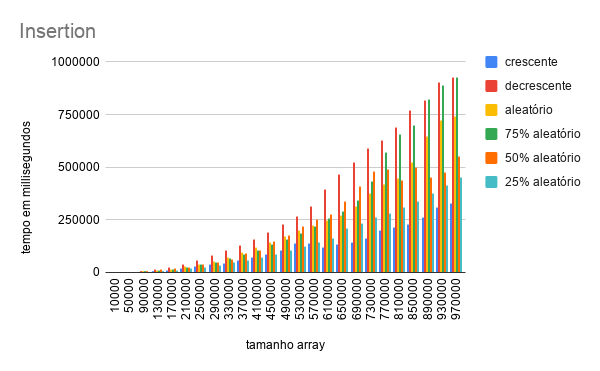
\includegraphics[width=1.1\textwidth, height=0.60\textwidth]{Insertion}
\end{figure}

\begin{figure}[!h]
	\caption{ Gráfico de linhas }
	\label{fig:insertion2}
	\centering
	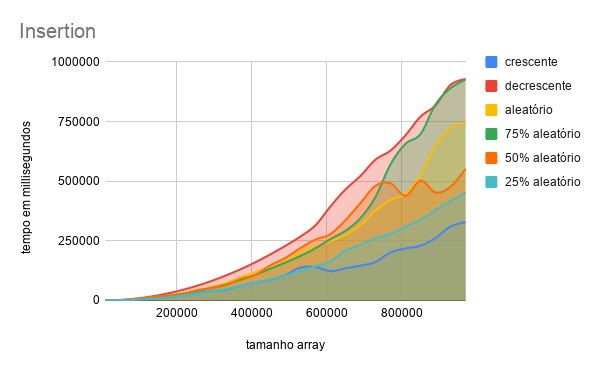
\includegraphics[width=1.1\textwidth, height=0.57\textwidth]{Insertion_linha}
\end{figure}


		\newpage
	\subsubsection{Selection Sort}
	Análise de tempo para o algoritmo de ordenação Selection Sort

		\begin{figure}[!h]
			\caption{ Gráfico de barras }
			\label{fig:selection1}
			\centering
	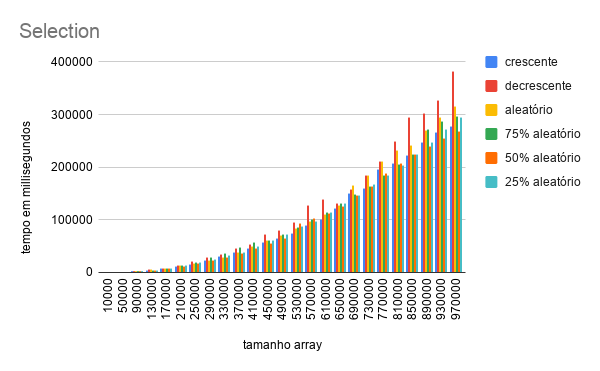
\includegraphics[width=1.1\textwidth, height=0.60\textwidth]{Selection}
		\end{figure}
		\begin{figure}[!h]
			\caption{ Gráfico de linhas }
			\label{fig:selection2}
			\centering
	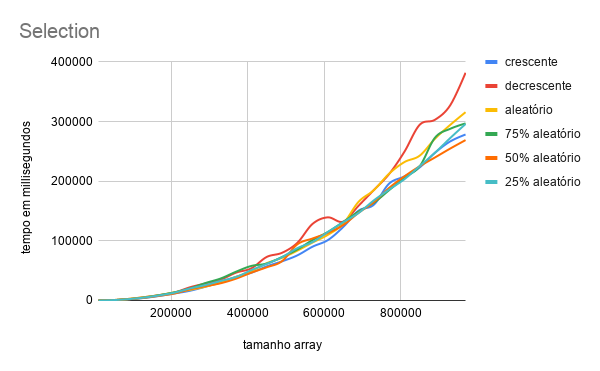
\includegraphics[width=1.1\textwidth, height=0.57\textwidth]{Selection_linha}
		\end{figure}


	\newpage
\subsubsection{Bubble Sort}
		 Análise de tempo para o algoritmo de ordenação Bubble Sort

\begin{figure}[!h]
	\caption{ Gráfico de barras }
	    \label{fig:bubble1}
	\centering
	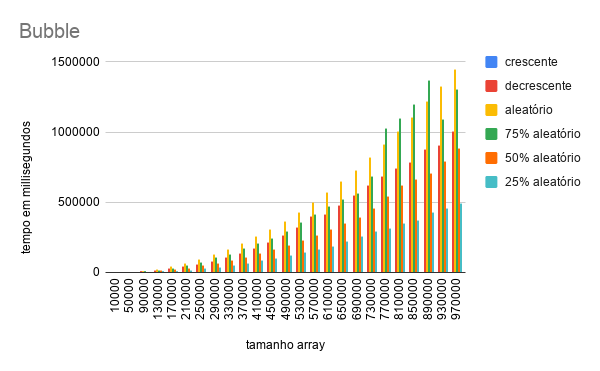
\includegraphics[width=1.1\textwidth, height=0.60\textwidth]{Bubble}
\end{figure}

	\begin{figure}[!h]
	\caption{ Gráfico de linhas }
	\label{fig:bubble2}
	\centering
	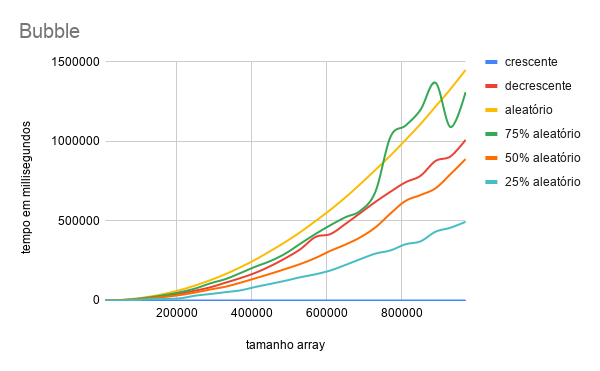
\includegraphics[width=1.1\textwidth, height=0.57\textwidth]{Bubble_linha}
\end{figure}



\subsubsection{Shell Sort}
Análise de tempo para o algoritmo de ordenação Shell Sort
	\begin{figure}[!h]
		\caption{ Gráfico de barras }
		\label{fig:shell1}
		\centering
		\includegraphics[width=1.1\textwidth, height=0.59\textwidth]{Shell }
	\end{figure}
	\begin{figure}[!h]
	\caption{ Gráfico de linhas }
	\label{fig:shell2}
	\centering
	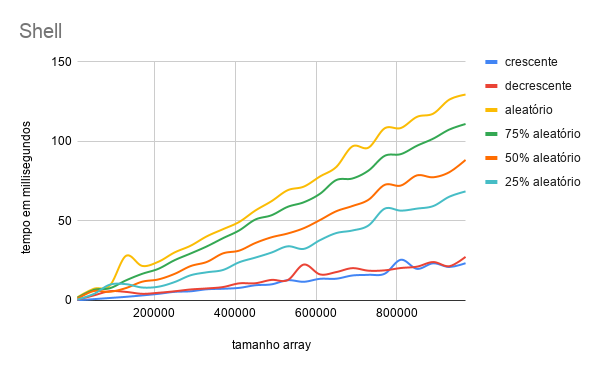
\includegraphics[width=1\textwidth, height=0.57\textwidth]{Shell_linha}
\end{figure}


	\newpage

\subsubsection{Quick Sort}
Análise de tempo para o algoritmo de ordenação Quick Sort

	\begin{figure}[!h]
		\caption{ Gráfico de barras }
		\label{fig:quick1}
		\centering
			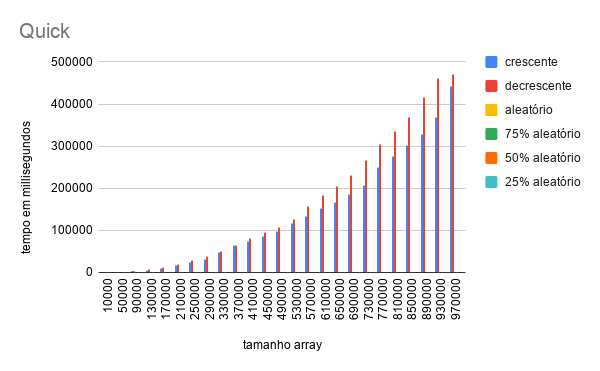
\includegraphics[width=1\textwidth, height=0.60\textwidth]{Quick}
	\end{figure}
	\begin{figure}[!h]
		\caption{ Gráfico de linhas }
		\label{fig:quick2}
		\centering
			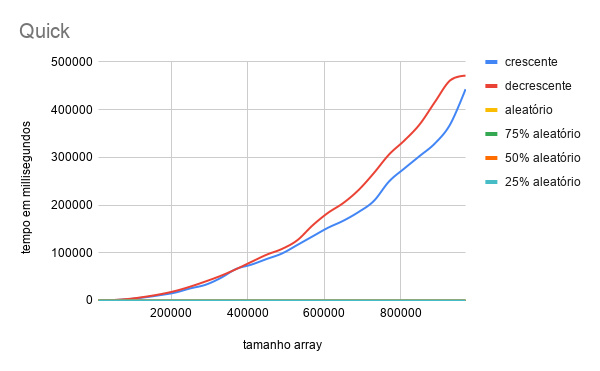
\includegraphics[width=1\textwidth, height=0.57\textwidth]{Quick_linha}
	\end{figure}
	\newpage

\subsubsection{Merge Sort}
Análise de tempo para o algoritmo de ordenação Merge Sort
	\begin{figure}[!h]
		\caption{ Gráfico de barras }
		\label{fig:merge1}
		\centering
			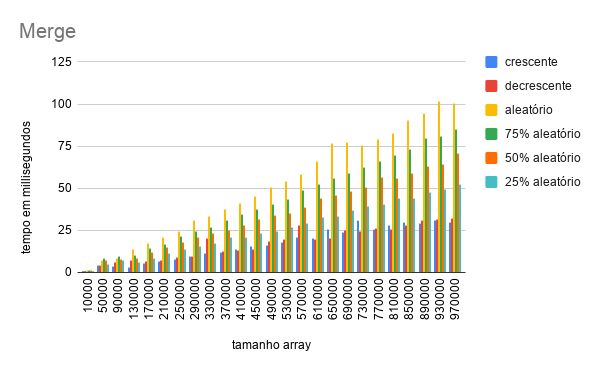
\includegraphics[width=1\textwidth, height=0.60\textwidth]{Merge}

	\end{figure}

	\begin{figure}[!h]
		\caption{ Gráfico de linhas }
		\label{fig:merge2}
		\centering
			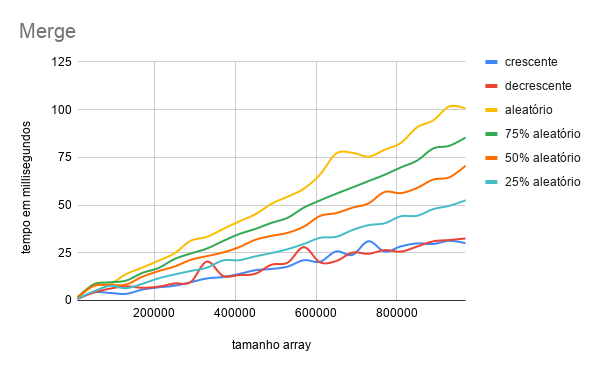
\includegraphics[width=1\textwidth, height=0.57\textwidth]{Merge _linha}
	\end{figure}


	\newpage
\subsubsection{Radix Sort}
Análise de tempo para o algoritmo de ordenação Radix Sort

	\begin{figure}[!h]
		\caption{ Gráfico de barras }
		\label{fig:radix1}
		\centering
	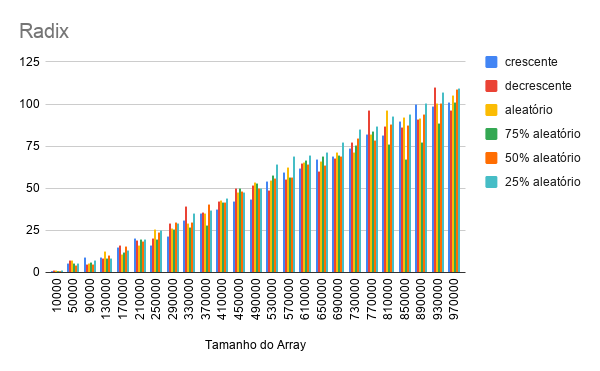
\includegraphics[width=1\textwidth, height=0.60\textwidth]{Radix}

	\end{figure}
	\begin{figure}[!h]
		\caption{ Gráfico de linhas }
		\label{fig:radix2}
		\centering
		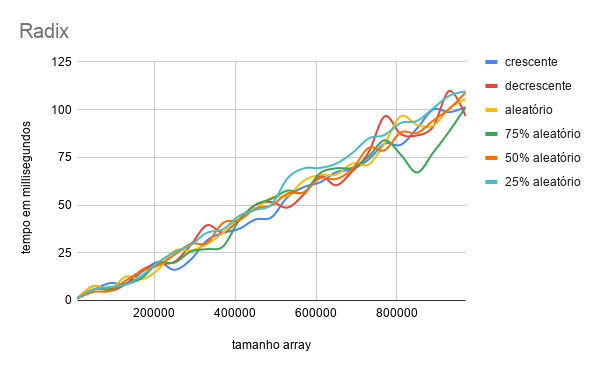
\includegraphics[width=1\textwidth, height=0.57\textwidth]{Radix_linha}
	\end{figure}




\newpage
\subsection{Gráficos - por tipo de amostra }


\subsubsection{Crescente}

	\begin{figure}[!h]
	\caption{ Gráfico de linhas }
	\label{fig:crescente1}
	\centering
	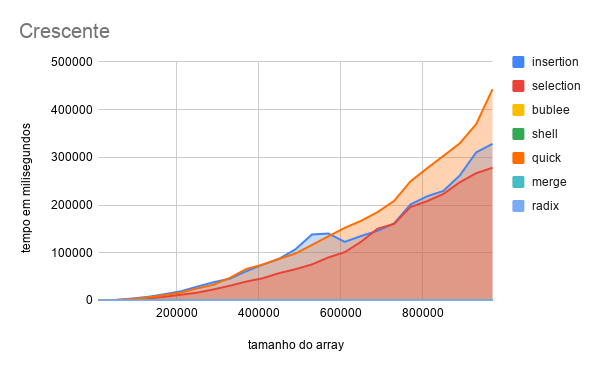
\includegraphics[width=1\textwidth, height=0.60\textwidth]{Crescente}
	
\end{figure}
\begin{figure}[!h]
	\caption{ Gráfico de linhas }
	\label{fig:crescente2}
	\centering
	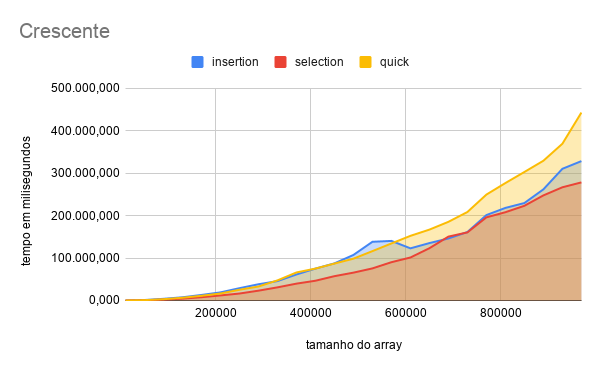
\includegraphics[width=1\textwidth, height=0.57\textwidth]{Crescente1}
\end{figure}

\begin{figure}[!h]
	\caption{ Gráfico de linhas }
	\label{fig:crescente3}
	\centering
	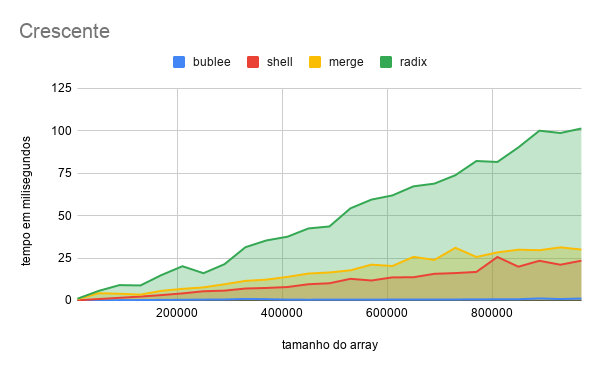
\includegraphics[width=1\textwidth, height=0.57\textwidth]{Crescente2}
\end{figure}
\newpage
\subsubsection{Decrescente}
	\begin{figure}[!h]
	\caption{ Gráfico de linhas }
	\label{fig:decrescente1}
	\centering
	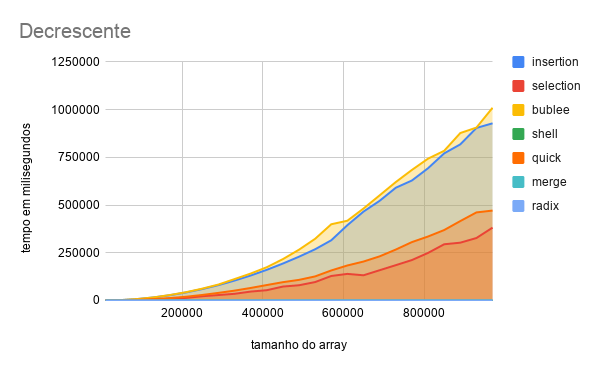
\includegraphics[width=1\textwidth, height=0.60\textwidth]{Decrescente}
	
\end{figure}
\begin{figure}[!h]
	\caption{ Gráfico de linhas }
	\label{fig:decrescente2}
	\centering
	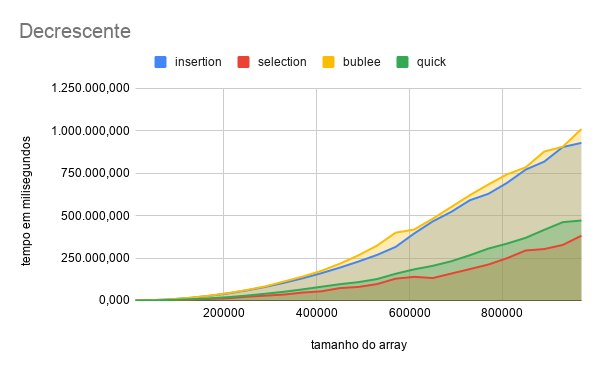
\includegraphics[width=1\textwidth, height=0.57\textwidth]{Decrescente1}
\end{figure}

\begin{figure}[!h]
	\caption{ Gráfico de linhas }
	\label{fig:decrescente3}
	\centering
	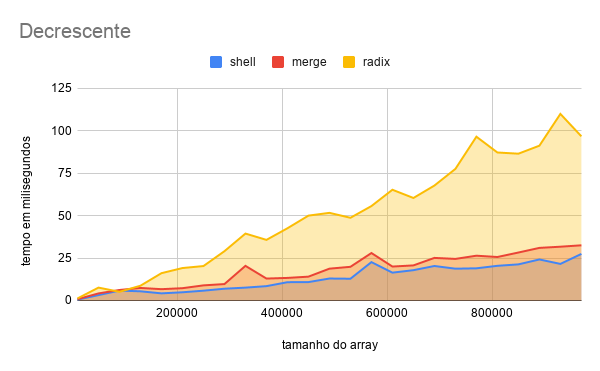
\includegraphics[width=1\textwidth, height=0.57\textwidth]{Decrescente2}
\end{figure}
\newpage

$  $ \\
\subsubsection{100\% Aleatória}

	\begin{figure}[!h]
	\caption{ Gráfico de linhas }
	\label{fig:random1}
	\centering
	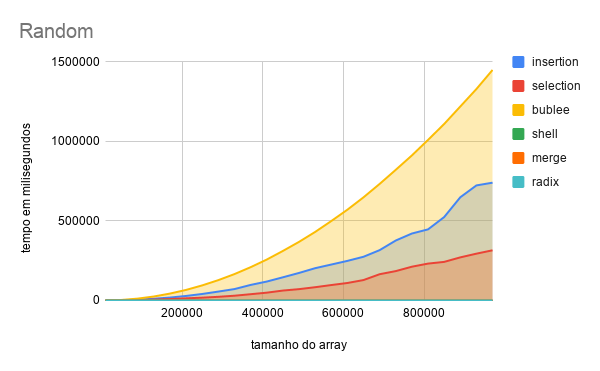
\includegraphics[width=1\textwidth, height=0.60\textwidth]{Random}
	
\end{figure}
\begin{figure}[!h]
	\caption{ Gráfico de linhas }
	\label{fig:random2}
	\centering
	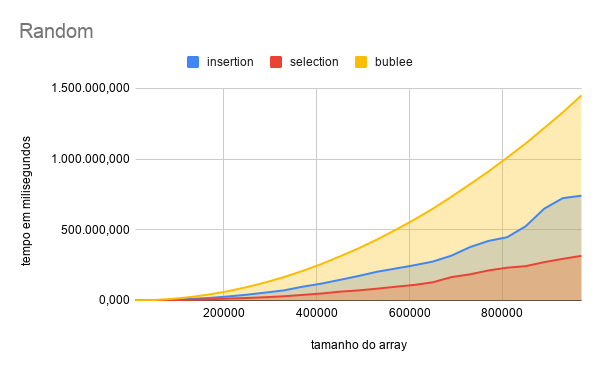
\includegraphics[width=1\textwidth, height=0.57\textwidth]{Random_1}
\end{figure}

\begin{figure}[!h]
	\caption{ Gráfico de linhas }
	\label{fig:random3}
	\centering
	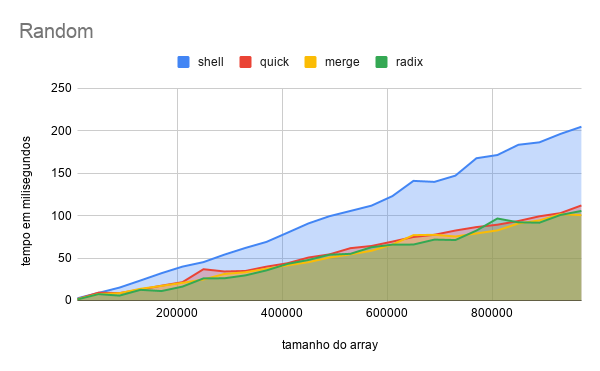
\includegraphics[width=1\textwidth, height=0.57\textwidth]{Random_2}
\end{figure}
\newpage


$  $ \\
\subsubsection{75\% Aleatória}
	\begin{figure}[!h]
	\caption{ Gráfico de linhas }
	\label{fig:75random1}
	\centering
	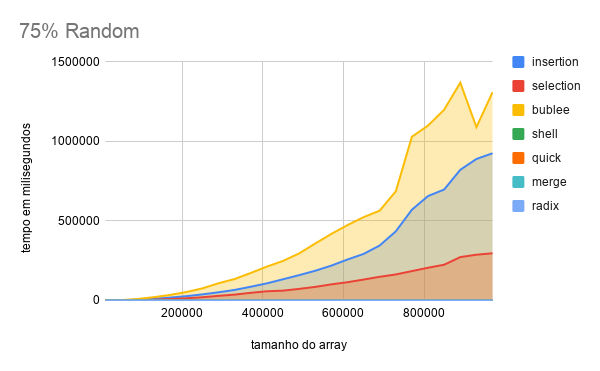
\includegraphics[width=1\textwidth, height=0.60\textwidth]{75Random}
	
\end{figure}
\begin{figure}[!h]
	\caption{ Gráfico de linhas }
	\label{fig:75random2}
	\centering
	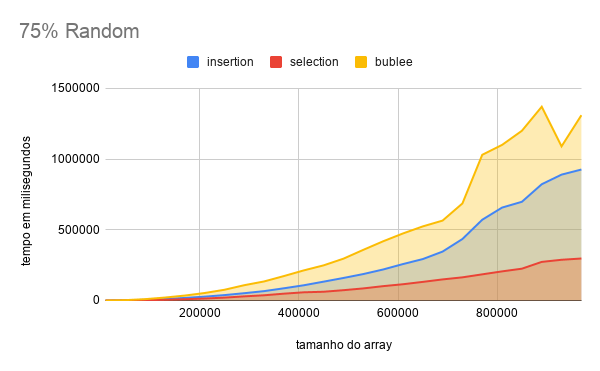
\includegraphics[width=1\textwidth, height=0.57\textwidth]{75Random1}
\end{figure}

\begin{figure}[!h]
	\caption{ Gráfico de linhas }
	\label{fig:75random3}
	\centering
	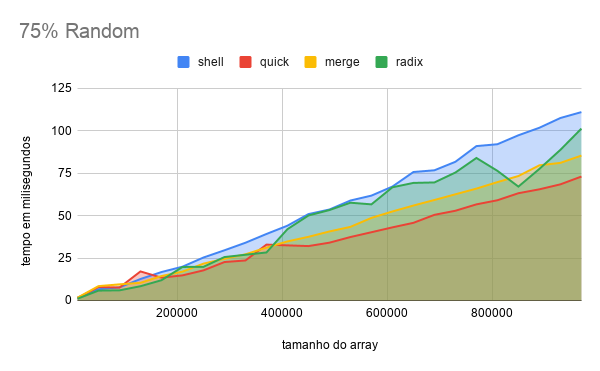
\includegraphics[width=1\textwidth, height=0.57\textwidth]{75Random2}
\end{figure}
\newpage


$  $  \\
 
\subsubsection{50\% Aleatória}
	\begin{figure}[!h]
	\caption{ Gráfico de linhas }
	\label{fig:50random1}
	\centering
	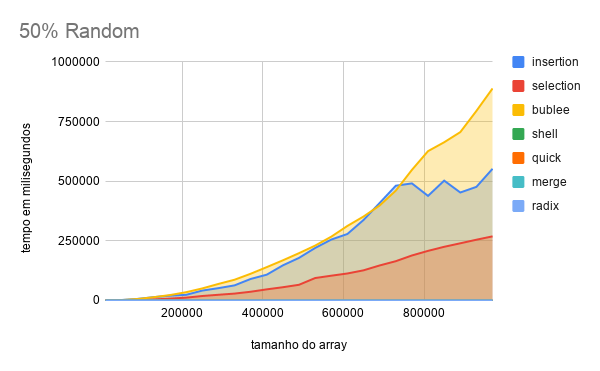
\includegraphics[width=1\textwidth, height=0.60\textwidth]{50Random}
	
\end{figure}
\begin{figure}[!h]
	\caption{ Gráfico de linhas }
	\label{fig:50random2}
	\centering
	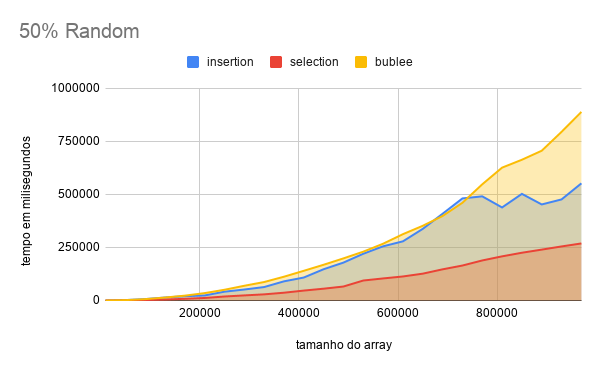
\includegraphics[width=1\textwidth, height=0.57\textwidth]{50Random1}
\end{figure}

\begin{figure}[!h]
	\caption{ Gráfico de linhas }
	\label{fig:50random3}
	\centering
	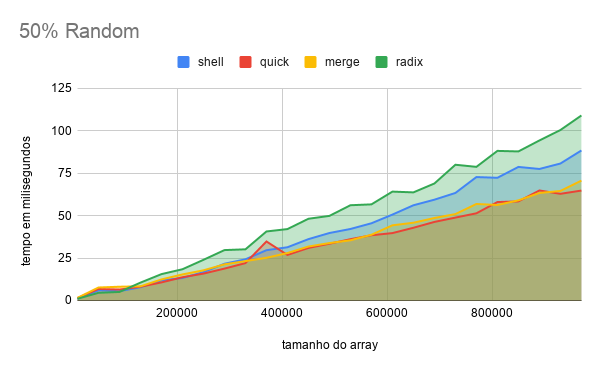
\includegraphics[width=1\textwidth, height=0.57\textwidth]{50Random2}
\end{figure}
\newpage


$  $ \\
\subsubsection{25\% Aleatória}
	\begin{figure}[!h]
	\caption{ Gráfico de linhas }
	\label{fig:25random1}
	\centering
	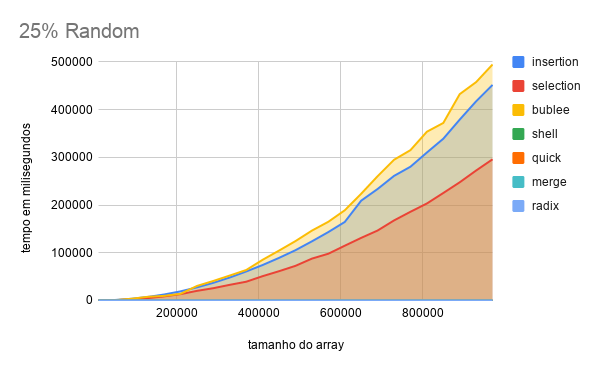
\includegraphics[width=1\textwidth, height=0.60\textwidth]{25Random}
	
\end{figure}
\begin{figure}[!h]
	\caption{ Gráfico de linhas }
	\label{fig:25random2}
	\centering
	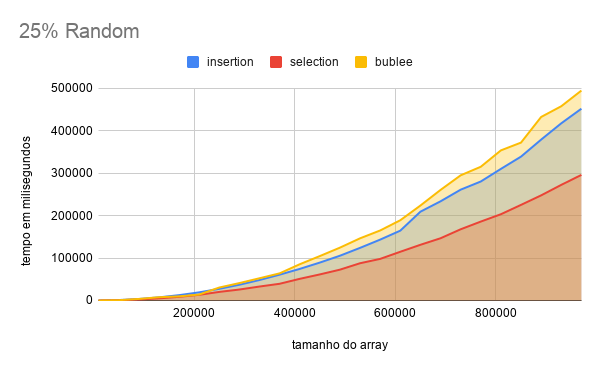
\includegraphics[width=1\textwidth, height=0.57\textwidth]{25Random1}
\end{figure}

\begin{figure}[!h]
	\caption{ Gráfico de linhas }
	\label{fig:25random3}
	\centering
	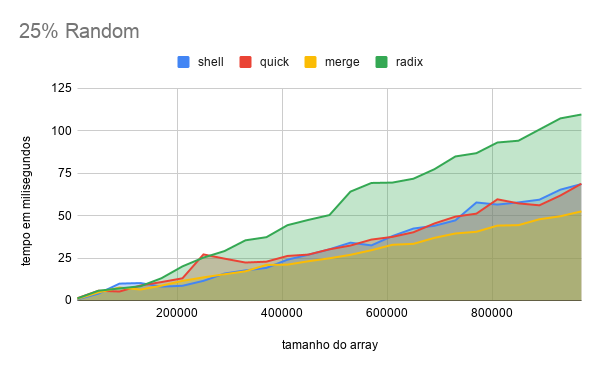
\includegraphics[width=1\textwidth, height=0.57\textwidth]{25Random2}
\end{figure}

\newpage


$  $ \\
	\newpage
	\section{Discussão}
	\subsection{Geral} 
		Para amostras crescentes, o insertion, selection e quick tem algorítimos ineficientes quando comparados com shell, merge, radix, e bubble sendo este ultimo claramente o mais eficiente para este caso. Já para amostras decrescentes, o insertion, bubble, selection e quick tem algorítimos ineficientes quando comparados com shell, merge e radix, como podemos ver o bubble passa de mais eficiente no caso de arrays em ordem crescente para estar entre os piores em ordem decrescente.
		\indent
		
		Para amostras em ordem aleatória, sendo totalmente aleatórias ou parcialmente, o insertion, selection e bubble tem algorítimos ineficientes quando comparados com shell, merge, radix, e quick.
	\subsection{Quais algoritmos para qual cenários?}
	
	\begin{enumerate}
		\item  elementos em ordem não decrescente - bubble
		\item  elemento em ordem não crescente - shell
		\item  elementos 100\% aleatórios - radix
		\item  75\% de seus elementos em sua posição definitiva - quick
		\item  25\% de seus elementos em sua posição definitiva - quick
		\item  50\% de seus elementos em sua posição definitiva - merge
	\end{enumerate}


	\subsection{Radix vs. Outros}
	O radix tem performance parecida em todos os tipos de amostra, ao contrario dos outros, com performances tão boas quanto, que variam dependendo da amostra.
	\subsection{Quick sort vs. Merge sort}
		Nas amostras crescente e decrescente o Merge sorte tem melhor performance.
		Já nas amostras aleatórias, pelos gráficos \ref{fig:random3}, \ref{fig:75random3}, \ref{fig:50random3}, \ref{fig:25random3}, é possível ver que quanto mais aleatório é a amostra a performance do Merge se torna ligeiramente pior que a do Quick sort.
	\subsection{Picos e Vales}
		Sim, provavelmente por causa de sobrecargas no sistema por estar executando tarefas paralelas.
	\subsection{Análise empírica vs. Análise matemática}
		Ambas são compatíveis.
		
		
	\newpage

	
	\addcontentsline{toc}{section}{Bibliografia}
	\section*{Bibliografia}
	\footnotesize{
		
		\noindent https://cmake.org/\\
		
	}
	\newpage
	\addcontentsline{toc}{section}{Anexo}
	\section*{Apêndice - Implementação dos algoritmos em CPP}



		\subsection{Função auxiliar para troca de posição}

	\begin{lstlisting}
  void swap(int * p1, int * p2) {
	int temp = * p1;
	* p1 = * p2;
	* p2 = temp;
}
	\end{lstlisting}


		\subsection{Insertion Sort}

\begin{lstlisting}
  void insertionsort(value_type * array, int size) {
	for (int i = 1; i < size; i++) {
		for (int j = i; j > 0; j--) {
			if (array[j - 1] > array[j]) {
				swap( & array[j], & array[j - 1]);
			}
		}
	}
}
\end{lstlisting}



	\subsection{Selection Sort}

\begin{lstlisting}
  void selectionsort(value_type * array, int size) {
	int i, j, min_value;
	for (i = 0; i < size - 1; i++) {
		min_value = i;
		for (j = i + 1; j < size; j++)
		if (array[j] < array[min_value])
		min_value = j;
		swap( & array[min_value], & array[i]);
	}
}
\end{lstlisting}



\subsection{Bubble Sort}

\begin{lstlisting}

void bubblesort(value_type * array, int size) {
	bool changed = false;
	int ordained = 0;
	do {
		changed = false;
		ordained++;
		for (int i = 0; i < (size - ordained); i++) {
			if (array[i + 1] < array[i]) {
				changed = true;
				swap( & array[i], & array[i + 1]);
			}
		}
	} while (changed);
}
\end{lstlisting}



\subsection{Shell Sort}

\begin{lstlisting}

void shellsort(value_type * array, int size) {
	for (int gap = size / 2; gap > 0; gap /= 2) {
	  for (int i = gap; i < size; i += 1) {
		int temp = array[i];
		int j;
		for (j = i; j >= gap && array[j - gap] > temp; j -= gap)
		  array[j] = array[j - gap];
		array[j] = temp;
	    }
	}
}
\end{lstlisting}



\subsection{Quick Sort}
\subsubsection{Passa do formato padrão (array, size) para o do Quick}
\begin{lstlisting}
  void quicksort(value_type * array, int size) {
	quicksort(array, 0, size - 1);
}

\end{lstlisting}


\subsubsection{Particiona}
\begin{lstlisting}
int partition(value_type * array, int low, int high) {
	int pivot = array[high];
	int i = (low - 1);
	for (int j = low; j <= high - 1; j++) {
		if (array[j] < pivot) {
			i++;
			swap( & array[i], & array[j]);
		}
	}
	swap( & array[i + 1], & array[high]);
	return (i + 1);
}
\end{lstlisting}


\subsubsection{Pricipal}
\begin{lstlisting}
  void quicksort(value_type * array, int l, int h) {
	int stack[h - l + 1];
	int top = -1;
	
	stack[++top] = l;
	stack[++top] = h;
	
	while (top >= 0) {
		h = stack[top--];
		l = stack[top--];
		
		int p = partition(array, l, h);
		if (p - 1 > l) {
			stack[++top] = l;
			stack[++top] = p - 1;
		}
		if (p + 1 < h) {
			stack[++top] = p + 1;
			stack[++top] = h;
		}
	}
}

\end{lstlisting}



\subsection{Merge Sort}
\subsubsection{Passa do formato padrão (array, size) para o do merge}
\begin{lstlisting}
	void mergesort(value_type * array, int size) {
		mergesort(array, 0, size - 1);
	}
\end{lstlisting}


\subsubsection{Pricipal que divide em 2 subarrays}
\begin{lstlisting}
	void mergesort(value_type * array, int l, int r) {
		if (l < r) {
			int m = l + (r - l) / 2;
			mergesort(array, l, m);
			mergesort(array, m + 1, r);
			merge(array, l, m, r);
		}
	}
\end{lstlisting}


\subsubsection{Função que mistura (merge) os 2 subarrays}
\begin{lstlisting}
	void merge(value_type * array, int l, int m, int r) {
		int i, j, k;
		int n1 = m - l + 1;
		int n2 = r - m;
		int left[n1], rigth[n2];
		
		for (i = 0; i < n1; i++)
		left[i] = array[l + i];
		for (j = 0; j < n2; j++)
		rigth[j] = array[m + 1 + j];
		
		i = 0;
		j = 0;
		k = l;
		while (i < n1 && j < n2) {
			if (left[i] <= rigth[j]) {
				array[k] = left[i];
				i++;
			} else {
				array[k] = rigth[j];
				j++;
			}
			k++;
		}
		
		while (i < n1) {
			array[k] = left[i];
			i++;
			k++;
		}
		while (j < n2) {
			array[k] = rigth[j];
			j++;
			k++;
		}
	}
	
}
\end{lstlisting}

\subsection{Radix Sort}
\begin{lstlisting}
  void radixsort(value_type * array, int size) {
	int i;
	value_type * b = new value_type[size];
	value_type maior = array[0];
	int exp = 1;
	for (i = 0; i < size; i++) {
		if (array[i] > maior)
		maior = array[i];
	}
	while (maior / exp > 0) {
		int count[10] = {
			0
		};
		for (i = 0; i < size; i++)
		count[(array[i] / exp) % 10]++;
		for (i = 1; i < 10; i++)
		count[i] += count[i - 1];
		for (i = size - 1; i >= 0; i--)
		b[--count[(array[i] / exp) % 10]] = array[i];
		for (i = 0; i < size; i++)
		array[i] = b[i];
		exp *= 10;
	}
	delete[] b;
}
\end{lstlisting}



\subsection{Codifo Gerar Array}
\subsubsection{Na ordem crescente}
\begin{lstlisting}
	for( auto i{0ull} ; i < tamanho_array ; ++i ){
		crescente[i]  = i;
	}
\end{lstlisting}

\subsubsection{Na ordem decrescente}
\begin{lstlisting}
	for( auto i{0ull} ; i < tamanho_array ; ++i ){
		decrescente[i]  = tamanho_array - i;
	}
\end{lstlisting}

\subsubsection{Aleatória}
\begin{lstlisting}
	for( auto i{0ull} ; i < tamanho_array ; ++i ){
		aleatorio[i]  = rand() % tamanho_array;
	}
\end{lstlisting}


\subsubsection{50\% aleatória}
\begin{lstlisting}
    for( auto i{0ull} ; i < tamanho_array ; ++i ){
	  aleatorio50[i] =  (i%2==0)  ? i :  rand() % tamanho_array;
    }
\end{lstlisting}



\subsubsection{75\% aleatória}
\begin{lstlisting}
    for( auto i{0ull} ; i < tamanho_array ; ++i ){
		 aleatorio75[i] =  (i%4==0)  ? i :  rand() % tamanho_array;
	}
\end{lstlisting}


\subsubsection{25\% aleatória}
\begin{lstlisting}
    for( auto i{0ull} ; i < tamanho_array ; ++i ){
		aleatorio25[i] =  (i%4!=0)  ? i :  rand() % tamanho_array;
	}
\end{lstlisting}
\end{document}



